\chapter{APPENDIX}
\newpage

\footnotesize

%%==========================================
\section{Glossary}
%==========================================
\paragraph{VIF - Varianve Inflation Factor}
quantifies how much the variance of a regression coefficient is inflated because its predictor is linearly correlated with other predictors (i.e., multicollinearity).


%==========================================
\section{Method Definition}
%==========================================

%------------------------------------------
\subsection{Variance Inflation Factor (VIF)}\label{subsec:vif}
%------------------------------------------

\paragraph{Definition.}
The \emph{Variance Inflation Factor} (VIF) quantifies how much the variance of an OLS coefficient is inflated due to linear dependence (multicollinearity) among predictors. For a given predictor $X_j$,
\[
\mathrm{VIF}_j \;=\; \frac{1}{1 - R_j^2},
\]
where $R_j^2$ is the coefficient of determination from the \emph{auxiliary regression} that regresses $X_j$ on all the other predictors $\{X_k: k\neq j\}$. If $X_j$ is orthogonal to the rest, $R_j^2{=}0$ and $\mathrm{VIF}_j{=}1$; as collinearity increases, $R_j^2\uparrow$ and $\mathrm{VIF}_j\uparrow$; under perfect collinearity, $R_j^2\to 1$ and $\mathrm{VIF}_j\to\infty$.

A related OLS variance identity makes the role of VIF explicit:
\[
\mathrm{Var}(\hat\beta_j) \;=\; \frac{\sigma^2}{\mathrm{SST}_j}\,\mathrm{VIF}_j,
\]
with $\mathrm{SST}_j=\sum_i (x_{ij}-\bar x_j)^2$ the total variation of $X_j$.

\paragraph{Computation (step-by-step).}
For each predictor $X_j$:
\begin{enumerate}
  \item Regress $X_j$ on the other predictors $\{X_k: k\neq j\}$ (auxiliary OLS).
  \item Record $R_j^2$ from that auxiliary regression.
  \item Compute $\mathrm{VIF}_j = 1/(1-R_j^2)$.
\end{enumerate}
Centering or standardizing does not change VIF, but can improve numerical stability. If the auxiliary regression is singular (perfect collinearity), VIF is undefined (effectively infinite).

\paragraph{Interpretation.}
Rule-of-thumb thresholds:
\begin{itemize}
  \item $\mathrm{VIF}\approx 1$: no multicollinearity concern,
  \item $\mathrm{VIF} > 5$: potentially problematic,
  \item $\mathrm{VIF} > 10$: generally considered high and worth action.
\end{itemize}

\paragraph{Actions for high VIF.}
\begin{itemize}
  \item \textbf{Remove or combine} redundant predictors (retain the more informative one).
  \item \textbf{Transform or re-encode} variables to reduce linear dependence.
  \item \textbf{Regularize} (e.g., ridge) if the goal is prediction and you prefer shrinkage over removal.
  \item \textbf{Iterative screen} (as used here): compute VIFs, drop the predictor with the largest VIF if it exceeds a threshold (e.g., 10), recompute, and repeat until all VIFs are below threshold.
\end{itemize}

\paragraph{Practical considerations.}
\begin{itemize}
  \item \textbf{Categorical predictors:} VIF is defined for single numeric columns. For multi-level categoricals represented by several dummies, a generalized measure (e.g., GVIF) is more appropriate. In our pipeline, VIF is applied only to \emph{continuous} features to avoid this complication.
  \item \textbf{Near-duplicates and composites:} Domain sums (e.g., FSum/BSum/PSum) and their constituents often create high VIFs; pairwise redundancy rules plus VIF mitigate this.
  \item \textbf{Small samples / near-singularity:} Expect unstable $R^2$ and large VIFs; consider dimensionality reduction or regularization.
\end{itemize}

\paragraph{Tiny example.}
With predictors $(X_1,X_2,X_3)$, to obtain $\mathrm{VIF}_2$: regress $X_2$ on $(X_1,X_3)$, say $R_2^2{=}0.84$, then $\mathrm{VIF}_2 = 1/(1-0.84)=6.25$, indicating moderate multicollinearity for $X_2$.


\newpage
%============================================
\section{Source Code for Feature Selection}
%============================================
\lstinputlisting[language=Python]{logs/FeatureSelection_ascii.py}

\newpage
%============================================
\section{Feature Selection Log}
%============================================
\begin{landscape}
\lstinputlisting[language=Python]{logs/FeatureSelectionLog_ascii.txt}
\end{landscape}

\newpage
%============================================
\section{Source Code for Model Base Class}
%============================================
\lstinputlisting[language=Python]{logs/base_model_ascii.py}


\newpage
%============================================
\section{Source Code for Model 1}
%============================================
\lstinputlisting[language=Python]{logs/model_1_reeval_ascii.py}

\IfFileExists{logs/model_1_log.txt}{
    \newpage
    \begin{landscape}
    %============================================
    \section{Computation Logs for Model 1}
    %============================================
    \lstinputlisting[inputencoding=utf8]{logs/model_1_log_ascii.txt}
    \end{landscape}
}{}

\newpage
%============================================
\section{Source Code for Model 2}
%============================================
\lstinputlisting[language=Python]{logs/model_2_gamma_ascii.py}

\IfFileExists{logs/model_2_log.txt}{
    \newpage
    \begin{landscape}
    %============================================
    \section{Computation Logs for Model 2}
    %============================================
    \lstinputlisting[inputencoding=utf8]{logs/model_2_log_ascii.txt}
    \end{landscape}
}{}

% \textsl{\newpage
% %============================================
% \section{Source Code for Model 3}
% %============================================
% \lstinputlisting[language=Python]{logs/model_3_robust_ascii.py}

% \IfFileExists{logs/model_3_log.txt}{
%     \newpage
%     \begin{landscape}
%     %============================================
%     \section{Computation Logs for Model 3}
%     %============================================
%     \lstinputlisting[inputencoding=utf8]{logs/model_3_log_ascii.txt}
%     \end{landscape}
% }{}

% \newpage
% %============================================
% \section{Source Code for Model 4}
% %============================================
% \lstinputlisting[language=Python]{logs/model_4_wls_ascii.py}

% \IfFileExists{logs/model_4_log.txt}{
%     \newpage
%     \begin{landscape}
%     %============================================
%     \section{Computation Logs for Model 4}
%     %============================================
%     \lstinputlisting[inputencoding=utf8]{logs/model_4_log_ascii.txt}
%     \end{landscape}
% }{}

% \newpage
% %============================================
% \section{Source Code for Model 5}
% %============================================
% \lstinputlisting[language=Python]{logs/model_5_ridge_ascii.py}

% \IfFileExists{logs/model_5_log.txt}{
%     \newpage
%     \begin{landscape}
%     %============================================
%     \section{Computation Logs for Model 5}
%     %============================================
%     \lstinputlisting[inputencoding=utf8]{logs/model_5_log_ascii.txt}
%     \end{landscape}
% }{}

% \newpage
% %============================================
% \section{Source Code for Model 6}
% %============================================
% \lstinputlisting[language=Python]{logs/model_6_lognormal_ascii.py}

% \IfFileExists{logs/model_6_log.txt}{
%     \newpage
%     \begin{landscape}
%     %============================================
%     \section{Computation Logs for Model 6}
%     %============================================
%     \lstinputlisting[inputencoding=utf8]{logs/model_6_log_ascii.txt}
%     \end{landscape}
% }{}

% \newpage
% %============================================
% \section{Source Code for Model 7}
% %============================================
% \lstinputlisting[language=Python]{logs/model_7_quantile_ascii.py}

% \IfFileExists{logs/model_7_log.txt}{
%     \newpage
%     \begin{landscape}
%     %============================================
%     \section{Computation Logs for Model 7}
%     %============================================
%     \lstinputlisting[inputencoding=utf8]{logs/model_7_log_ascii.txt}
%     \end{landscape}
% }{}

% \newpage
% %============================================
% \section{Source Code for Model 8}
% %============================================
% \lstinputlisting[language=Python]{logs/model_8_bayesian_ascii.py}

% \IfFileExists{logs/model_8_log.txt}{
%     \newpage
%     \begin{landscape}
%     %============================================
%     \section{Computation Logs for Model 8}
%     %============================================
%     \lstinputlisting[inputencoding=utf8]{logs/model_8_log_ascii.txt}
%     \end{landscape}
% }{}

% \newpage
% %============================================
% \section{Source Code for Model 9}
% %============================================
% \lstinputlisting[language=Python]{logs/model_9_random_forest_ascii.py}

% \IfFileExists{logs/model_9_log.txt}{
%     \newpage
%     \begin{landscape}
%     %============================================
%     \section{Computation Logs for Model 9}
%     %============================================
%     \lstinputlisting[inputencoding=utf8]{logs/model_9_log_ascii.txt}
%     \end{landscape}
% }{}

% \newpage
% %============================================
% \section{Source Code for Model 10}
% %============================================
% \lstinputlisting[language=Python]{logs/model_10_neural_ascii.py}

% \IfFileExists{logs/model_10_log.txt}{
%     \newpage
%     \begin{landscape}
%     %============================================
%     \section{Computation Logs for Model 10}
%     %============================================
%     \lstinputlisting[inputencoding=utf8]{logs/model_10_log_ascii.txt}
%     \end{landscape}
% }{}

% }

\section{Data Provided by APD for Modeling}
\begin{landscape}

\subsection{sysdiagrams}

\subsubsection{Table Overview}
\begin{itemize}
\item \textbf{Table Name:} sysdiagrams
\item \textbf{Schema:} dbo
\item \textbf{Number of Records:} 0
\item \textbf{Number of Columns:} 5
\end{itemize}

\subsubsection{Column Details}
\begin{longtable}{|l|l|l|r|p{6cm}|}
\hline
\textbf{Column Name} & \textbf{Data Type} & \textbf{Description} & \textbf{N} & \textbf{Statistics/Values} \\
\hline
\endfirsthead
\multicolumn{5}{c}{\textit{Continued from previous page}} \\
\hline
\textbf{Column Name} & \textbf{Data Type} & \textbf{Description} & \textbf{N} & \textbf{Statistics/Values} \\
\hline
\endhead
\hline
\multicolumn{5}{c}{\textit{Continued on next page}} \\
\endfoot
\hline
\endlastfoot
name & nvarchar(128) &  & 0 & All NULL values \\
\hline
principal\_id & int(10) &  & 0 & All NULL values \\
\hline
diagram\_id & int(10) &  & 0 & All NULL values \\
\hline
version & int(10) &  & 0 & All NULL values \\
\hline
definition & varbinary(-1) &  & 0 & All NULL values \\
\hline
\end{longtable}

\subsection{tbl\_Budgets}

\subsubsection{Table Overview}
\begin{itemize}
\item \textbf{Table Name:} tbl\_Budgets
\item \textbf{Schema:} dbo
\item \textbf{Number of Records:} 219,457
\item \textbf{Number of Columns:} 19
\end{itemize}

\subsubsection{Column Details}
\begin{longtable}{|l|l|l|r|p{6cm}|}
\hline
\textbf{Column Name} & \textbf{Data Type} & \textbf{Description} & \textbf{N} & \textbf{Statistics/Values} \\
\hline
\endfirsthead
\multicolumn{5}{c}{\textit{Continued from previous page}} \\
\hline
\textbf{Column Name} & \textbf{Data Type} & \textbf{Description} & \textbf{N} & \textbf{Statistics/Values} \\
\hline
\endhead
\hline
\multicolumn{5}{c}{\textit{Continued on next page}} \\
\endfoot
\hline
\endlastfoot
CaseNo & bigint(19) &  & 42093 & Range: [10184.00, 100198.00], Avg: 39353.87, Median: 35849.00 \\
\hline
BudgetID & bigint(19) &  & 219457 & Range: [66.00, 219554.00], Avg: 109819.48, Median: 109821.00 \\
\hline
BudgetType & varchar(100) &  & 2 & \{CDC+, iBudget\} \\
\hline
BudgetStatus & varchar(100) &  & 4 & \{Budget Approved, Approved, Terminated, Draft\} \\
\hline
FiscalYear & varchar(100) &  & 6 & \{2026, 2024, 2021, 2022, 2025, 2023\} \\
\hline
Programs & varchar(75) &  & 2 & \{CDC+, APD Waiver\} \\
\hline
WSC & varchar(100) &  & 1031 & ... \\
\hline
ApprovedBy & int(10) &  & 6 & Range: [1182.00, 34038.00], Avg: 9428.56, Median: 2487.00 \\
\hline
ApprovalDate & datetime &  & 15 & Range: [2020-05-22, 2025-05-21] \\
\hline
StartDate & datetime &  & 271 & Range: [2020-07-01, 2025-07-22] \\
\hline
EndDate & datetime &  & 6 & Range: [2021-06-30, 2026-06-30] \\
\hline
BudgetAmount & numeric(19,2) &  & 146839 & Range: [-28280.29, 894542.33], Avg: 58144.60, Median: 49936.11 \\
\hline
AnnualizedAmount & numeric(19,2) &  & 131128 & Range: [-54617.64, 485174942.72], Avg: 61506.63, Median: 51322.04 \\
\hline
AmountEncumbered & numeric(19,2) &  & 147533 & Range: [0.00, 1236377.20], Avg: 50557.89, Median: 41775.08 \\
\hline
AmountUnauthorized & numeric(19,2) &  & 121870 & Range: [-1073148.93, 850693.76], Avg: 9621.87, Median: 1882.51 \\
\hline
PrioriBudgetAmount & numeric(19,2) &  & 150649 & Range: [0.00, 1144471.65], Avg: 52194.31, Median: 43875.48 \\
\hline
Comments & varchar(-1) &  & 121 & ... \\
\hline
UserStamp & varchar(100) &  & 61 & ... \\
\hline
DateTimeStamp & datetime &  & 49148 & Range: [2020-05-25, 2025-09-11] \\
\hline
\end{longtable}

\subsection{tbl\_Claims\_MMIS}

\subsubsection{Table Overview}
\begin{itemize}
\item \textbf{Table Name:} tbl\_Claims\_MMIS
\item \textbf{Schema:} dbo
\item \textbf{Number of Records:} 37,750,736
\item \textbf{Number of Columns:} 20
\end{itemize}

\subsubsection{Column Details}
\begin{longtable}{|l|l|l|r|p{6cm}|}
\hline
\textbf{Column Name} & \textbf{Data Type} & \textbf{Description} & \textbf{N} & \textbf{Statistics/Values} \\
\hline
\endfirsthead
\multicolumn{5}{c}{\textit{Continued from previous page}} \\
\hline
\textbf{Column Name} & \textbf{Data Type} & \textbf{Description} & \textbf{N} & \textbf{Statistics/Values} \\
\hline
\endhead
\hline
\multicolumn{5}{c}{\textit{Continued on next page}} \\
\endfoot
\hline
\endlastfoot
CaseNo & bigint(19) &  & 41285 & Range: [10184.00, 99376.00], Avg: 36590.87, Median: 33566.00 \\
\hline
PIN & varchar(20) &  & 41267 & ... \\
\hline
ProviderName & varchar(500) &  & 5249 & ... \\
\hline
ProviderMedcId & varchar(20) &  & 5004 & ... \\
\hline
ProcCode & varchar(20) &  & 156 & ... \\
\hline
ServiceDate & datetime &  & 1886 & Range: [2020-07-01, 2025-08-29] \\
\hline
Units & int(10) &  & 1958 & Range: [-98112.00, 98112.00], Avg: 17.94, Median: 15.00 \\
\hline
BilledAmt & numeric(9,2) &  & 47855 & Range: [-25270.05, 36622.37], Avg: 191.90, Median: 101.40 \\
\hline
PaidAmt & numeric(9,2) &  & 46066 & Range: [-21173.51, 26975.48], Avg: 191.69, Median: 101.40 \\
\hline
PaidDate & datetime &  & 541 & Range: [2020-07-03, 2025-09-03] \\
\hline
ICN & varchar(100) &  & 11172269 & ... \\
\hline
AdjustICN & varchar(100) &  & 407203 & ... \\
\hline
TreatingProvMedcId & varchar(20) &  & 1869 & ... \\
\hline
TransType & char(1) &  & 0 & All NULL values \\
\hline
LineNmbr & varchar(20) &  & 51 & ... \\
\hline
PA & varchar(20) &  & 811384 & ... \\
\hline
ClaimType & char(1) &  & 2 & \{P, V\} \\
\hline
ClaimSubType & char(1) &  & 3 & \{R, O, A\} \\
\hline
CreateDate & datetime &  & 276 & Range: [2020-07-17, 2025-09-08] \\
\hline
Id & bigint(19) &  & 37750736 & Range: [1.00, 37750736.00], Avg: 18875368.50, Median: 18875369.00 \\
\hline
\end{longtable}

\subsection{tbl\_ConsumerContacts}

\subsubsection{Table Overview}
\begin{itemize}
\item \textbf{Table Name:} tbl\_ConsumerContacts
\item \textbf{Schema:} dbo
\item \textbf{Number of Records:} 433,650
\item \textbf{Number of Columns:} 11
\end{itemize}

\subsubsection{Column Details}
\begin{longtable}{|l|l|l|r|p{6cm}|}
\hline
\textbf{Column Name} & \textbf{Data Type} & \textbf{Description} & \textbf{N} & \textbf{Statistics/Values} \\
\hline
\endfirsthead
\multicolumn{5}{c}{\textit{Continued from previous page}} \\
\hline
\textbf{Column Name} & \textbf{Data Type} & \textbf{Description} & \textbf{N} & \textbf{Statistics/Values} \\
\hline
\endhead
\hline
\multicolumn{5}{c}{\textit{Continued on next page}} \\
\endfoot
\hline
\endlastfoot
CONTACTID & bigint(19) &  & 262802 & Range: [10468.00, 444197.00], Avg: 219587.19, Median: 208125.00 \\
\hline
FIRSTNAME & varchar(30) &  & 61717 & ... \\
\hline
LASTNAME & varchar(30) &  & 82349 & ... \\
\hline
GENDER & varchar(100) &  & 3 & \{, Female, Male\} \\
\hline
CASENO & bigint(19) &  & 73402 & Range: [10184.00, 101016.00], Avg: 41002.77, Median: 36889.00 \\
\hline
RELATIONSHIP & varchar(100) &  & 85 & ... \\
\hline
Multirelationship & varchar(-1) &  & 5236 & ... \\
\hline
Active & int(10) &  & 2 & Range: [0.00, 1.00], Avg: 0.87, Median: 1.00 \\
\hline
DateTimeStamp & datetime2 &  & 409847 & Range: [2018-11-27, 2025-09-12] \\
\hline
UserStamp & varchar(100) &  & 3437 & ... \\
\hline
RECID & bigint(19) &  & 433650 & Range: [10174.00, 504002.00], Avg: 252246.06, Median: 267038.00 \\
\hline
\end{longtable}

\subsection{tbl\_Consumers}

\subsubsection{Table Overview}
\begin{itemize}
\item \textbf{Table Name:} tbl\_Consumers
\item \textbf{Schema:} dbo
\item \textbf{Number of Records:} 60,821
\item \textbf{Number of Columns:} 66
\end{itemize}

\subsubsection{Column Details}
\begin{longtable}{|l|l|l|r|p{6cm}|}
\hline
\textbf{Column Name} & \textbf{Data Type} & \textbf{Description} & \textbf{N} & \textbf{Statistics/Values} \\
\hline
\endfirsthead
\multicolumn{5}{c}{\textit{Continued from previous page}} \\
\hline
\textbf{Column Name} & \textbf{Data Type} & \textbf{Description} & \textbf{N} & \textbf{Statistics/Values} \\
\hline
\endhead
\hline
\multicolumn{5}{c}{\textit{Continued on next page}} \\
\endfoot
\hline
\endlastfoot
CASENO & bigint(19) &  & 60821 & Range: [10184.00, 100986.00], Avg: 49458.02, Median: 48467.00 \\
\hline
DOB & datetime &  & 21369 & Range: [1926-11-08, 2022-07-16] \\
\hline
GENDER & varchar(100) &  & 2 & \{Male, Female\} \\
\hline
RACE & varchar(100) &  & 7 & \{Asian/Pacific Islander, Other, , Alaska Native, Native American, Caucasian, African American\} \\
\hline
PLANGUAGE & varchar(100) &  & 18 & ... \\
\hline
SLANGUAGE & varchar(100) &  & 21 & ... \\
\hline
TITLE & varchar(50) &  & 51 & ... \\
\hline
ETHNICITYLOOKUP & varchar(30) &  & 17 & ... \\
\hline
County & varchar(100) &  & 119 & ... \\
\hline
District & varchar(25) &  & 39 & ... \\
\hline
Region & varchar(100) &  & 25 & ... \\
\hline
DOD & datetime &  & 161 & Range: [2018-12-29, 2025-09-09] \\
\hline
CauseOfDeath & varchar(1000) &  & 171 & ... \\
\hline
DODAction & varchar(50) &  & 2 & \{Verified Alive, \} \\
\hline
DODFileNumber & varchar(25) &  & 181 & ... \\
\hline
RESIDENCETYPE & varchar(100) &  & 28 & ... \\
\hline
MedicaidId & varchar(500) &  & 54141 & ... \\
\hline
ABCPIN & varchar(50) &  & 49469 & ... \\
\hline
ReferralSource & varchar(100) &  & 25 & ... \\
\hline
CBCFlag & bit &  & 2 & Range: [0.00, 1.00], Avg: 0.00, Median: 0.00 \\
\hline
ReferredToVR & varchar(50) &  & 4 & \{Yes, No, NA, \} \\
\hline
ANNUALINCOME & numeric(19,2) &  & 1879 & Range: [0.00, 86400.00], Avg: 1884.71, Median: 0.00 \\
\hline
Competency & varchar(50) &  & 12 & ... \\
\hline
Status & varchar(10) &  & 1 & \{Active\} \\
\hline
DevelopmentalDisability & varchar(-1) &  & 87 & ... \\
\hline
FUNDCODE & varchar(25) &  & 1 & \{APD\} \\
\hline
DISPOSITION & varchar(100) &  & 9 & \{APD Eligible - Bypass PE, APD Eligible - PESC Assigned, APD Eligible - ICF/SNF Transition, APD Eligible - Pre-enrollment, APD Eligible - DDMC, APD Eligible - High Risk, APD Eligible - Waiver, APD Eligible - NonWaiver, APD Eligible - ICF/IID\} \\
\hline
DISPOSITIONDATE & datetime &  & 7089 & Range: [1948-03-15, 2025-09-11] \\
\hline
OPENDATE & datetime &  & 11324 & Range: [1948-03-15, 2025-09-10] \\
\hline
OPENREASON & varchar(-1) &  & 3 & \{, 1, 0\} \\
\hline
CLOSEDATE & datetime &  & 14 & Range: [2022-07-09, 2025-08-26] \\
\hline
CLOSEREASON & varchar(100) &  & 6 & \{Deceased, Loss of Contact, Not Eligible, Services No Longer Appropriate, , Services No Longer Needed\} \\
\hline
ApplicationReceivedDate & datetime &  & 10621 & Range: [1889-07-11, 2025-09-11] \\
\hline
ApplicationReceivedViaOAS & varchar(50) &  & 2 & \{Yes, No\} \\
\hline
ApplicantRequestingCWE & varchar(50) &  & 2 & \{Yes, No\} \\
\hline
RequiresSOPTReview & varchar(10) &  & 2 & \{Yes, No\} \\
\hline
DateAssignedToSOPT & datetime &  & 72 & Range: [2024-10-02, 2025-09-10] \\
\hline
SOPTName & varchar(100) &  & 53 & ... \\
\hline
DateSOPTCompletedReview & datetime &  & 71 & Range: [2024-11-19, 2025-09-11] \\
\hline
OPENID & bigint(19) &  & 60816 & Range: [10211.00, 106665.00], Avg: 50706.64, Median: 49173.00 \\
\hline
PRIMARYWORKER & varchar(100) &  & 1296 & ... \\
\hline
PRIMARYWORKERID & bigint(19) &  & 1329 & Range: [330.00, 52864.00], Avg: 16773.24, Median: 3881.00 \\
\hline
SECONDWORKER & varchar(100) &  & 89 & ... \\
\hline
SECONDWORKERID & bigint(19) &  & 89 & Range: [359.00, 51214.00], Avg: 1442.13, Median: 1182.00 \\
\hline
PrimaryDiagnosis & varchar(200) &  & 15 & ... \\
\hline
SecondaryDiagnosis & varchar(200) &  & 14 & ... \\
\hline
OtherDiagnosis & varchar(200) &  & 23 & ... \\
\hline
MentalHealthDiag1 & varchar(200) &  & 56 & ... \\
\hline
MentalHealthDiag2 & varchar(200) &  & 52 & ... \\
\hline
MentalHealthDiag3 & varchar(200) &  & 43 & ... \\
\hline
MentalHealthDiag4 & varchar(200) &  & 27 & ... \\
\hline
MentalHealthDiag\_5\_6 & varchar(100) &  & 75 & ... \\
\hline
REVIEW & varchar(100) &  & 8 & \{Initial Application, Initial, As Needed, Other, Monthly, Update/Amended , Quarterly, Annual\} \\
\hline
REVIEWDATE & datetime &  & 6168 & Range: [1976-07-01, 2025-09-11] \\
\hline
SSNMonthlyBenefitAmt & varchar(50) &  & 3147 & ... \\
\hline
3rdPartyHealthInsurance & varchar(50) &  & 3 & \{Yes, No, \} \\
\hline
CompetitivelyEmployed & varchar(50) &  & 3 & \{Yes, No, \} \\
\hline
HireDate & varchar(50) &  & 1632 & ... \\
\hline
AvgMonthlyEarnings & varchar(50) &  & 1083 & ... \\
\hline
WantsEmployment & varchar(50) &  & 3 & \{Yes, No, \} \\
\hline
HourlyWage & varchar(50) &  & 259 & ... \\
\hline
MinimumWage & varchar(50) &  & 3 & \{Yes, No, \} \\
\hline
CONTACTID & bigint(19) &  & 60821 & Range: [10467.00, 443946.00], Avg: 102913.53, Median: 79348.00 \\
\hline
DateTimeStamp & datetime &  & 58726 & Range: [2018-11-27, 2025-09-12] \\
\hline
UserStamp & varchar(100) &  & 1641 & ... \\
\hline
Id & int(10) &  & 60821 & Range: [1.00, 96453.00], Avg: 40810.13, Median: 39363.00 \\
\hline
\end{longtable}

\subsection{tbl\_Diagnosis}

\subsubsection{Table Overview}
\begin{itemize}
\item \textbf{Table Name:} tbl\_Diagnosis
\item \textbf{Schema:} dbo
\item \textbf{Number of Records:} 74,826
\item \textbf{Number of Columns:} 12
\end{itemize}

\subsubsection{Column Details}
\begin{longtable}{|l|l|l|r|p{6cm}|}
\hline
\textbf{Column Name} & \textbf{Data Type} & \textbf{Description} & \textbf{N} & \textbf{Statistics/Values} \\
\hline
\endfirsthead
\multicolumn{5}{c}{\textit{Continued from previous page}} \\
\hline
\textbf{Column Name} & \textbf{Data Type} & \textbf{Description} & \textbf{N} & \textbf{Statistics/Values} \\
\hline
\endhead
\hline
\multicolumn{5}{c}{\textit{Continued on next page}} \\
\endfoot
\hline
\endlastfoot
CASENO & bigint(19) &  & 74330 & Range: [10184.00, 100986.00], Avg: 48488.48, Median: 47484.00 \\
\hline
FUNDCODE & varchar(25) &  & 3 & \{APD, INC, FOR\} \\
\hline
PrimaryDiagnosis & varchar(200) &  & 19 & ... \\
\hline
SecondaryDiagnosis & varchar(200) &  & 21 & ... \\
\hline
TertiaryDiagnosis & varchar(200) &  & 27 & ... \\
\hline
QuaternaryDiagnosis & varchar(200) &  & 27 & ... \\
\hline
REVIEW & varchar(100) &  & 8 & \{Initial Application, Initial, As Needed, Other, Monthly, Update/Amended , Quarterly, Annual\} \\
\hline
REVIEWDATE & datetime &  & 6597 & Range: [1976-07-01, 2025-09-11] \\
\hline
STATUS & varchar(100) &  & 4 & \{Pending, Open, Complete, Draft\} \\
\hline
DATETIMESTAMP & datetime &  & 11325 & Range: [2018-12-06, 2025-09-11] \\
\hline
UserStamp & varchar(100) &  & 140 & ... \\
\hline
DiagnosisID & bigint(19) &  & 74826 & Range: [79.00, 74922.00], Avg: 37494.67, Median: 37493.00 \\
\hline
\end{longtable}

\subsection{tbl\_EZBudget}

\subsubsection{Table Overview}
\begin{itemize}
\item \textbf{Table Name:} tbl\_EZBudget
\item \textbf{Schema:} dbo
\item \textbf{Number of Records:} 43,213
\item \textbf{Number of Columns:} 41
\end{itemize}

\subsubsection{Column Details}
\begin{longtable}{|l|l|l|r|p{6cm}|}
\hline
\textbf{Column Name} & \textbf{Data Type} & \textbf{Description} & \textbf{N} & \textbf{Statistics/Values} \\
\hline
\endfirsthead
\multicolumn{5}{c}{\textit{Continued from previous page}} \\
\hline
\textbf{Column Name} & \textbf{Data Type} & \textbf{Description} & \textbf{N} & \textbf{Statistics/Values} \\
\hline
\endhead
\hline
\multicolumn{5}{c}{\textit{Continued on next page}} \\
\endfoot
\hline
\endlastfoot
CASENO & bigint(19) &  & 29004 & Range: [10184.00, 100397.00], Avg: 46922.21, Median: 45362.00 \\
\hline
REVIEW & varchar(100) &  & 7 & \{Initial Application, Initial, As Needed, Other, Update/Amended, Quarterly, Annual\} \\
\hline
Worker & varchar(100) &  & 640 & ... \\
\hline
ReviewDate & datetime &  & 1927 & Range: [2017-12-27, 2025-09-05] \\
\hline
STATUS & varchar(100) &  & 6 & \{Signature Complete, Pending, Open, Submitted, Complete, Draft\} \\
\hline
Division & varchar(25) &  & 1 & \{APD\} \\
\hline
ApprovedBy & varchar(100) &  & 280 & ... \\
\hline
ApprovedDate & datetime &  & 2070 & Range: [2018-12-06, 2025-09-05] \\
\hline
Region & varchar(50) &  & 7 & \{Northeast, Southeast, Central, , Southern, Suncoast, Northwest\} \\
\hline
UpdateSituation & varchar(50) &  & 6 & \{Change in age, Change in living setting, When SANs is requested, At the time of waiver enrollment for new waiver en, , Change in QSI\} \\
\hline
LivingSetting & varchar(50) &  & 7 & \{Family Home, CTEP or Special Medical Home Care, Standard or Live-In Residential Habilitatio, , Behavior Focus Residential Habilitation, Intensive Behavior Residential Habilitation, Independent Living, Supported Living, or Licensed \} \\
\hline
CurrentAge & varchar(50) &  & 89 & ... \\
\hline
PropFactor & varchar(50) &  & 1 & \{1.00288\} \\
\hline
QSIBehavioralScore & varchar(50) &  & 25 & ... \\
\hline
QSIFunctionalScore & varchar(50) &  & 45 & ... \\
\hline
Q14 & varchar(50) &  & 5 & \{3, 2, 1, 0, 4\} \\
\hline
Q15 & varchar(50) &  & 5 & \{3, 2, 1, 0, 4\} \\
\hline
Q16 & varchar(50) &  & 5 & \{3, 2, 1, 0, 4\} \\
\hline
Q17 & varchar(50) &  & 5 & \{3, 2, 1, 0, 4\} \\
\hline
Q18 & varchar(50) &  & 5 & \{3, 2, 1, 0, 4\} \\
\hline
Q19 & varchar(50) &  & 5 & \{3, 2, 1, 0, 4\} \\
\hline
Q20 & varchar(50) &  & 5 & \{3, 2, 1, 0, 4\} \\
\hline
Q21 & varchar(50) &  & 5 & \{3, 2, 1, 0, 4\} \\
\hline
Q22 & varchar(50) &  & 5 & \{3, 2, 1, 0, 4\} \\
\hline
Q23 & varchar(50) &  & 5 & \{3, 2, 1, 0, 4\} \\
\hline
Q24 & varchar(50) &  & 5 & \{3, 2, 1, 0, 4\} \\
\hline
Q25 & varchar(50) &  & 5 & \{3, 2, 1, 0, 4\} \\
\hline
Q26 & varchar(50) &  & 5 & \{3, 2, 1, 0, 4\} \\
\hline
Q27 & varchar(50) &  & 5 & \{3, 2, 1, 0, 4\} \\
\hline
Q28 & varchar(50) &  & 5 & \{3, 2, 1, 0, 4\} \\
\hline
Q29 & varchar(50) &  & 5 & \{3, 2, 1, 0, 4\} \\
\hline
Q30 & varchar(50) &  & 5 & \{3, 2, 1, 0, 4\} \\
\hline
Q33 & varchar(50) &  & 5 & \{3, 2, 1, 0, 4\} \\
\hline
Q34 & varchar(50) &  & 5 & \{3, 2, 1, 0, 4\} \\
\hline
Q36 & varchar(50) &  & 5 & \{3, 2, 1, 0, 4\} \\
\hline
Q43 & varchar(50) &  & 2 & \{0, 4\} \\
\hline
Q44 & varchar(50) &  & 5 & \{3, 2, 1, 0, 4\} \\
\hline
DATETIMESTAMP & datetime &  & 43207 & Range: [2018-12-07, 2025-09-05] \\
\hline
UserStamp & varchar(100) &  & 328 & ... \\
\hline
EZBudgetAssessId & bigint(19) &  & 43213 & Range: [72383.00, 1396021.00], Avg: 651351.83, Median: 584652.00 \\
\hline
AlgorithmAmt & float(53) &  & 33513 & Range: [762.41, 203765.83], Avg: 33179.24, Median: 25468.61 \\
\hline
\end{longtable}

\subsection{tbl\_Model5b\_Predictions}

\subsubsection{Table Overview}
\begin{itemize}
\item \textbf{Table Name:} tbl\_Model5b\_Predictions
\item \textbf{Schema:} dbo
\item \textbf{Number of Records:} 0
\item \textbf{Number of Columns:} 19
\end{itemize}

\subsubsection{Column Details}
\begin{longtable}{|l|l|l|r|p{6cm}|}
\hline
\textbf{Column Name} & \textbf{Data Type} & \textbf{Description} & \textbf{N} & \textbf{Statistics/Values} \\
\hline
\endfirsthead
\multicolumn{5}{c}{\textit{Continued from previous page}} \\
\hline
\textbf{Column Name} & \textbf{Data Type} & \textbf{Description} & \textbf{N} & \textbf{Statistics/Values} \\
\hline
\endhead
\hline
\multicolumn{5}{c}{\textit{Continued on next page}} \\
\endfoot
\hline
\endlastfoot
PredictionID & bigint(19) &  & 0 & All NULL values \\
\hline
CaseNo & bigint(19) &  & 0 & All NULL values \\
\hline
AssessID & bigint(19) &  & 0 & All NULL values \\
\hline
ReviewDate & datetime &  & 0 & All NULL values \\
\hline
LivingSetting & varchar(10) &  & 0 & All NULL values \\
\hline
Age & int(10) &  & 0 & All NULL values \\
\hline
AgeGroup & varchar(20) &  & 0 & All NULL values \\
\hline
BSum & int(10) &  & 0 & All NULL values \\
\hline
FSum & int(10) &  & 0 & All NULL values \\
\hline
PSum & int(10) &  & 0 & All NULL values \\
\hline
FHFSum & int(10) &  & 0 & All NULL values \\
\hline
SLFSum & int(10) &  & 0 & All NULL values \\
\hline
SLBSum & int(10) &  & 0 & All NULL values \\
\hline
SqrtPrediction & decimal(19,4) &  & 0 & All NULL values \\
\hline
PredictedBudget & decimal(19,2) &  & 0 & All NULL values \\
\hline
CalculationDate & datetime &  & 0 & All NULL values \\
\hline
CreatedDate & datetime &  & 0 & All NULL values \\
\hline
CreatedBy & varchar(100) &  & 0 & All NULL values \\
\hline
RunID & bigint(19) &  & 0 & All NULL values \\
\hline
\end{longtable}

\subsection{tbl\_PlannedServices}

\subsubsection{Table Overview}
\begin{itemize}
\item \textbf{Table Name:} tbl\_PlannedServices
\item \textbf{Schema:} dbo
\item \textbf{Number of Records:} 1,066,576
\item \textbf{Number of Columns:} 33
\end{itemize}

\subsubsection{Column Details}
\begin{longtable}{|l|l|l|r|p{6cm}|}
\hline
\textbf{Column Name} & \textbf{Data Type} & \textbf{Description} & \textbf{N} & \textbf{Statistics/Values} \\
\hline
\endfirsthead
\multicolumn{5}{c}{\textit{Continued from previous page}} \\
\hline
\textbf{Column Name} & \textbf{Data Type} & \textbf{Description} & \textbf{N} & \textbf{Statistics/Values} \\
\hline
\endhead
\hline
\multicolumn{5}{c}{\textit{Continued on next page}} \\
\endfoot
\hline
\endlastfoot
CaseNo & bigint(19) &  & 41919 & Range: [10184.00, 100198.00], Avg: 37730.16, Median: 34374.00 \\
\hline
Division & varchar(25) &  & 1 & \{APD\} \\
\hline
FiscalYear & int(10) &  & 6 & Range: [2021.00, 2026.00], Avg: 2023.44, Median: 2023.00 \\
\hline
STARTDATE & datetime &  & 1961 & Range: [2020-07-01, 2026-06-20] \\
\hline
ENDDATE & datetime &  & 2140 & Range: [2020-07-01, 2026-06-30] \\
\hline
IndexSubObjectCode & varchar(100) &  & 12 & ... \\
\hline
ServiceRatio & varchar(100) &  & 11 & ... \\
\hline
ConsumerCounty & varchar(100) &  & 67 & ... \\
\hline
GeographicDifferential & varchar(100) &  & 3 & \{Geographic, Monroe, Non-Geographic\} \\
\hline
ProviderRateType & varchar(100) &  & 2 & \{Agency, Solo\} \\
\hline
ServiceCode & varchar(25) &  & 135 & ... \\
\hline
Service & varchar(100) &  & 135 & ... \\
\hline
UnitType & varchar(100) &  & 8 & \{15 mins, Day, Hour, Item, Mile, Month, Trip, Units\} \\
\hline
UnitsPer & numeric(19,2) &  & 4264 & Range: [0.00, 30816.00], Avg: 224.27, Median: 24.00 \\
\hline
UnitsOfMeasure & varchar(25) &  & 7 & \{, Business Day, Calendar Day, Month - Round Up, Quarter, Week, Year\} \\
\hline
TotalUnits & numeric(19,4) &  & 12525 & Range: [0.00, 35136.00], Avg: 1168.33, Median: 96.00 \\
\hline
AnnualizedUnits & int(10) &  & 10424 & Range: [0.00, 74887844.00], Avg: 2285.11, Median: 21.00 \\
\hline
VendorID & bigint(19) &  & 5550 & Range: [10055.00, 26323.00], Avg: 14224.89, Median: 13638.00 \\
\hline
ProviderName & varchar(75) &  & 5518 & ... \\
\hline
ProviderMedcId & varchar(20) &  & 5524 & ... \\
\hline
Rate & numeric(19,4) &  & 9296 & Range: [0.00, 135497.45], Avg: 429.10, Median: 14.51 \\
\hline
MaxAmount & numeric(19,2) &  & 102179 & Range: [0.00, 323705.76], Avg: 10655.39, Median: 2178.60 \\
\hline
COMMENTS & varchar(-1) &  & 578178 & ... \\
\hline
PlannedServiceStatus & varchar(100) &  & 10 & \{, Approved, Proposed, Region Review Approved, Region Review Denied, Region Review Partially Approved, State Review Approved, State Review Denied, State Review Partially Approved, Terminated\} \\
\hline
RegionStateReviewComments & varchar(5000) &  & 310592 & ... \\
\hline
AllowEVVDelivery & bit &  & 2 & Range: [0.00, 1.00], Avg: 0.15, Median: 0.00 \\
\hline
EVVComments & varchar(500) &  & 33 & ... \\
\hline
DATETIMESTAMP & datetime &  & 468520 & Range: [2020-06-01, 2025-09-12] \\
\hline
UserStamp & varchar(100) &  & 1726 & ... \\
\hline
PlannedServiceId & bigint(19) &  & 1066576 & Range: [501.00, 1238183.00], Avg: 635362.07, Median: 640598.00 \\
\hline
PlanId & bigint(19) &  & 220989 & Range: [1.00, 232993.00], Avg: 116411.38, Median: 117959.00 \\
\hline
ISComboCodeID & bigint(19) &  & 14 & Range: [71.00, 110.00], Avg: 93.19, Median: 95.00 \\
\hline
VendorServicesId & bigint(19) &  & 54897 & Range: [46092.00, 1278384.00], Avg: 964743.70, Median: 944077.00 \\
\hline
\end{longtable}

\subsection{tbl\_Plans}

\subsubsection{Table Overview}
\begin{itemize}
\item \textbf{Table Name:} tbl\_Plans
\item \textbf{Schema:} dbo
\item \textbf{Number of Records:} 221,814
\item \textbf{Number of Columns:} 17
\end{itemize}

\subsubsection{Column Details}
\begin{longtable}{|l|l|l|r|p{6cm}|}
\hline
\textbf{Column Name} & \textbf{Data Type} & \textbf{Description} & \textbf{N} & \textbf{Statistics/Values} \\
\hline
\endfirsthead
\multicolumn{5}{c}{\textit{Continued from previous page}} \\
\hline
\textbf{Column Name} & \textbf{Data Type} & \textbf{Description} & \textbf{N} & \textbf{Statistics/Values} \\
\hline
\endhead
\hline
\multicolumn{5}{c}{\textit{Continued on next page}} \\
\endfoot
\hline
\endlastfoot
CaseNo & bigint(19) &  & 41975 & Range: [10184.00, 100198.00], Avg: 39451.24, Median: 35976.00 \\
\hline
Division & varchar(25) &  & 1 & \{APD\} \\
\hline
Program & varchar(75) &  & 5 & \{Non-Waiver, CDC+, ICF/IID, APD Waiver, DDMC\} \\
\hline
Worker & varchar(100) &  & 2011 & ... \\
\hline
CreationDate & datetime &  & 1646 & Range: [2004-05-14, 2026-06-30] \\
\hline
Comments & varchar(-1) &  & 4685 & ... \\
\hline
Status & varchar(100) &  & 5 & \{No Review Required, Pending, Approved, Complete, Draft\} \\
\hline
BeginDate & datetime &  & 1396 & Range: [2019-07-01, 2025-09-11] \\
\hline
EndDate & datetime &  & 811 & Range: [2020-06-30, 2026-07-01] \\
\hline
Review & varchar(50) &  & 8 & \{Northeast, Southeast, State Office, Central, , Southern, Suncoast, Northwest\} \\
\hline
ReviewRequestDate & datetime &  & 1932 & Range: [2002-03-23, 8202-08-14] \\
\hline
UserStamp & varchar(100) &  & 1286 & ... \\
\hline
DateTimeStamp & datetime &  & 166735 & Range: [2020-05-25, 2025-09-12] \\
\hline
PlanId & bigint(19) &  & 221814 & Range: [1.00, 232993.00], Avg: 120111.93, Median: 121818.00 \\
\hline
BudgetId & bigint(19) &  & 215902 & Range: [66.00, 219548.00], Avg: 110245.49, Median: 110512.00 \\
\hline
OpenId & bigint(19) &  & 41988 & Range: [10211.00, 105804.00], Avg: 40108.08, Median: 36479.00 \\
\hline
EnrollID & bigint(19) &  & 44473 & Range: [10459.00, 298912.00], Avg: 57207.99, Median: 35547.00 \\
\hline
\end{longtable}

\subsection{tbl\_QSIAssessments}

\subsubsection{Table Overview}
\begin{itemize}
\item \textbf{Table Name:} tbl\_QSIAssessments
\item \textbf{Schema:} dbo
\item \textbf{Number of Records:} 90,467
\item \textbf{Number of Columns:} 61
\end{itemize}

\subsubsection{Column Details}
\begin{longtable}{|l|l|l|r|p{6cm}|}
\hline
\textbf{Column Name} & \textbf{Data Type} & \textbf{Description} & \textbf{N} & \textbf{Statistics/Values} \\
\hline
\endfirsthead
\multicolumn{5}{c}{\textit{Continued from previous page}} \\
\hline
\textbf{Column Name} & \textbf{Data Type} & \textbf{Description} & \textbf{N} & \textbf{Statistics/Values} \\
\hline
\endhead
\hline
\multicolumn{5}{c}{\textit{Continued on next page}} \\
\endfoot
\hline
\endlastfoot
CASENO & bigint(19) &  & 53022 & Range: [10184.00, 100332.00], Avg: 43620.79, Median: 40795.00 \\
\hline
ABCPIN & varchar(50) &  & 45269 & ... \\
\hline
STATUS & varchar(100) &  & 5 & \{Pending, Open, Submitted, Complete, Draft\} \\
\hline
REVIEW & varchar(100) &  & 8 & \{Initial Application, Initial, As Needed, Other, Monthly, Update/Amended, Quarterly, Annual\} \\
\hline
REVIEWDATE & datetime &  & 2668 & Range: [2000-01-01, 2025-09-05] \\
\hline
RATER & varchar(100) &  & 198 & ... \\
\hline
RaterID & bigint(19) &  & 199 & Range: [344.00, 51822.00], Avg: 7479.66, Median: 2123.00 \\
\hline
COMMENTS & text(2147483647) &  & 0 & All NULL values \\
\hline
APPROVEDBY & varchar(100) &  & 205 & ... \\
\hline
APPROVEDATE & datetime &  & 2315 & Range: [2018-12-04, 2025-09-05] \\
\hline
Q13a & varchar(50) &  & 3 & \{Yes, No, \} \\
\hline
Q13b & varchar(50) &  & 3 & \{Yes, No, \} \\
\hline
Q13c & varchar(50) &  & 3 & \{Yes, No, \} \\
\hline
Q14 & varchar(50) &  & 5 & \{3, 2, 1, 0, 4\} \\
\hline
Q15 & varchar(50) &  & 5 & \{3, 2, 1, 0, 4\} \\
\hline
Q16 & varchar(50) &  & 5 & \{3, 2, 1, 0, 4\} \\
\hline
Q17 & varchar(50) &  & 5 & \{3, 2, 1, 0, 4\} \\
\hline
Q18 & varchar(50) &  & 5 & \{3, 2, 1, 0, 4\} \\
\hline
Q19 & varchar(50) &  & 5 & \{3, 2, 1, 0, 4\} \\
\hline
Q20 & varchar(50) &  & 5 & \{3, 2, 1, 0, 4\} \\
\hline
Q21 & varchar(50) &  & 5 & \{3, 2, 1, 0, 4\} \\
\hline
Q22 & varchar(50) &  & 5 & \{3, 2, 1, 0, 4\} \\
\hline
Q23 & varchar(50) &  & 5 & \{3, 2, 1, 0, 4\} \\
\hline
Q24 & varchar(50) &  & 5 & \{3, 2, 1, 0, 4\} \\
\hline
Q25 & varchar(50) &  & 5 & \{3, 2, 1, 0, 4\} \\
\hline
Q26 & varchar(50) &  & 5 & \{3, 2, 1, 0, 4\} \\
\hline
Q27 & varchar(50) &  & 5 & \{3, 2, 1, 0, 4\} \\
\hline
Q28 & varchar(50) &  & 5 & \{3, 2, 1, 0, 4\} \\
\hline
Q29 & varchar(50) &  & 5 & \{3, 2, 1, 0, 4\} \\
\hline
Q30 & varchar(50) &  & 5 & \{3, 2, 1, 0, 4\} \\
\hline
Q31a & varchar(50) &  & 3 & \{Yes, No, \} \\
\hline
Q31b & varchar(50) &  & 35 & ... \\
\hline
Q32 & varchar(50) &  & 5 & \{3, 2, 1, 0, 4\} \\
\hline
Q33 & varchar(50) &  & 6 & \{3, 2, , 1, 0, 4\} \\
\hline
Q34 & varchar(50) &  & 5 & \{3, 2, 1, 0, 4\} \\
\hline
Q35 & varchar(50) &  & 5 & \{3, 2, 1, 0, 4\} \\
\hline
Q36 & varchar(50) &  & 5 & \{3, 2, 1, 0, 4\} \\
\hline
Q37 & varchar(50) &  & 5 & \{3, 2, 1, 0, 4\} \\
\hline
Q38 & varchar(50) &  & 5 & \{3, 2, 1, 0, 4\} \\
\hline
Q39 & varchar(50) &  & 5 & \{3, 2, 1, 0, 4\} \\
\hline
Q40 & varchar(50) &  & 5 & \{3, 2, 1, 0, 4\} \\
\hline
Q41 & varchar(50) &  & 5 & \{3, 2, 1, 0, 4\} \\
\hline
Q42 & varchar(50) &  & 5 & \{3, 2, 1, 0, 4\} \\
\hline
Q43 & varchar(50) &  & 2 & \{0, 4\} \\
\hline
Q44 & varchar(50) &  & 5 & \{3, 2, 1, 0, 4\} \\
\hline
Q45 & varchar(50) &  & 5 & \{3, 2, 1, 0, 4\} \\
\hline
Q46 & varchar(50) &  & 5 & \{3, 2, 1, 0, 4\} \\
\hline
Q47 & varchar(50) &  & 5 & \{3, 2, 1, 0, 4\} \\
\hline
Q48 & varchar(50) &  & 5 & \{3, 2, 1, 0, 4\} \\
\hline
Q49 & varchar(50) &  & 5 & \{3, 2, 1, 0, 4\} \\
\hline
Q50 & varchar(50) &  & 5 & \{3, 2, 1, 0, 4\} \\
\hline
Q51a & varchar(50) &  & 3 & \{Yes, No, \} \\
\hline
FLEVEL & varchar(50) &  & 7 & \{3, 2, 6, , 1, 5, 4\} \\
\hline
BLEVEL & varchar(50) &  & 7 & \{3, 2, 6, , 1, 5, 4\} \\
\hline
PLEVEL & varchar(50) &  & 7 & \{3, 2, 6, , 1, 5, 4\} \\
\hline
OLEVEL & varchar(50) &  & 6 & \{Minimal, Intensive, , Moderate, Extensive, Basic\} \\
\hline
LOSRI & varchar(50) &  & 6 & \{3, 2, , 1, 5, 4\} \\
\hline
DATETIMESTAMP & datetime &  & 87317 & Range: [2018-12-04, 2025-09-05] \\
\hline
UserStamp & varchar(100) &  & 216 & ... \\
\hline
AssessID & bigint(19) &  & 90467 & Range: [72322.00, 1396019.00], Avg: 633710.68, Median: 603107.00 \\
\hline
LegacyAssessID & bigint(19) &  & 41912 & Range: [1.00, 171589.00], Avg: 44866.57, Median: 29605.00 \\
\hline
\end{longtable}

\subsection{tbl\_QSIAssessmentsLegacy}

\subsubsection{Table Overview}
\begin{itemize}
\item \textbf{Table Name:} tbl\_QSIAssessmentsLegacy
\item \textbf{Schema:} dbo
\item \textbf{Number of Records:} 171,358
\item \textbf{Number of Columns:} 55
\end{itemize}

\subsubsection{Column Details}
\begin{longtable}{|l|l|l|r|p{6cm}|}
\hline
\textbf{Column Name} & \textbf{Data Type} & \textbf{Description} & \textbf{N} & \textbf{Statistics/Values} \\
\hline
\endfirsthead
\multicolumn{5}{c}{\textit{Continued from previous page}} \\
\hline
\textbf{Column Name} & \textbf{Data Type} & \textbf{Description} & \textbf{N} & \textbf{Statistics/Values} \\
\hline
\endhead
\hline
\multicolumn{5}{c}{\textit{Continued on next page}} \\
\endfoot
\hline
\endlastfoot
ABCPIN & varchar(10) &  & 63886 & ... \\
\hline
STATUS & varchar(10) &  & 2 & \{Incomplete, Complete\} \\
\hline
REVIEW & varchar(7) &  & 2 & \{Initial, Annual\} \\
\hline
REVIEWDATE & datetime &  & 171358 & Range: [2008-01-22, 2018-11-30] \\
\hline
RATER & varchar(61) &  & 440 & ... \\
\hline
RATERID & int(10) &  & 432 & Range: [104.00, 3051.00], Avg: 749.33, Median: 354.00 \\
\hline
APPROVEDBY & varchar(61) &  & 429 & ... \\
\hline
CompletedDate & datetime &  & 168640 & Range: [2008-01-22, 2018-12-18] \\
\hline
Q14 & int(10) &  & 5 & Range: [0.00, 4.00], Avg: 0.32, Median: 0.00 \\
\hline
Q15 & int(10) &  & 5 & Range: [0.00, 4.00], Avg: 0.17, Median: 0.00 \\
\hline
Q16 & int(10) &  & 5 & Range: [0.00, 4.00], Avg: 0.82, Median: 0.00 \\
\hline
Q17 & int(10) &  & 5 & Range: [0.00, 4.00], Avg: 0.72, Median: 0.00 \\
\hline
Q18 & int(10) &  & 5 & Range: [0.00, 4.00], Avg: 0.60, Median: 0.00 \\
\hline
Q19 & int(10) &  & 5 & Range: [0.00, 4.00], Avg: 1.40, Median: 1.00 \\
\hline
Q20 & int(10) &  & 5 & Range: [0.00, 4.00], Avg: 1.98, Median: 2.00 \\
\hline
Q21 & int(10) &  & 5 & Range: [0.00, 4.00], Avg: 1.63, Median: 1.00 \\
\hline
Q22 & int(10) &  & 5 & Range: [0.00, 4.00], Avg: 1.28, Median: 1.00 \\
\hline
Q23 & int(10) &  & 5 & Range: [0.00, 4.00], Avg: 2.59, Median: 3.00 \\
\hline
Q24 & int(10) &  & 5 & Range: [0.00, 4.00], Avg: 1.92, Median: 2.00 \\
\hline
Q25 & int(10) &  & 5 & Range: [0.00, 4.00], Avg: 0.92, Median: 0.00 \\
\hline
Q26 & int(10) &  & 5 & Range: [0.00, 4.00], Avg: 1.05, Median: 0.00 \\
\hline
Q27 & int(10) &  & 5 & Range: [0.00, 4.00], Avg: 0.80, Median: 0.00 \\
\hline
Q28 & int(10) &  & 5 & Range: [0.00, 4.00], Avg: 0.36, Median: 0.00 \\
\hline
Q29 & int(10) &  & 5 & Range: [0.00, 4.00], Avg: 0.50, Median: 0.00 \\
\hline
Q30 & int(10) &  & 5 & Range: [0.00, 4.00], Avg: 1.29, Median: 1.00 \\
\hline
Q30a & int(10) &  & 2 & Range: [0.00, 1.00], Avg: 0.10, Median: 0.00 \\
\hline
Q30b & int(10) &  & 6 & Range: [0.00, 5.00], Avg: 1.33, Median: 1.00 \\
\hline
Q30bOther & varchar(50) &  & 441 & ... \\
\hline
Q31 & int(10) &  & 5 & Range: [0.00, 4.00], Avg: 0.52, Median: 0.00 \\
\hline
Q32 & int(10) &  & 5 & Range: [0.00, 4.00], Avg: 0.30, Median: 0.00 \\
\hline
Q33 & int(10) &  & 5 & Range: [0.00, 4.00], Avg: 0.12, Median: 0.00 \\
\hline
Q34 & int(10) &  & 5 & Range: [0.00, 4.00], Avg: 0.26, Median: 0.00 \\
\hline
Q35 & int(10) &  & 5 & Range: [0.00, 4.00], Avg: 0.97, Median: 0.00 \\
\hline
Q36 & int(10) &  & 5 & Range: [0.00, 4.00], Avg: 0.71, Median: 0.00 \\
\hline
Q37 & int(10) &  & 5 & Range: [0.00, 4.00], Avg: 0.61, Median: 0.00 \\
\hline
Q38 & int(10) &  & 5 & Range: [0.00, 4.00], Avg: 0.48, Median: 0.00 \\
\hline
Q39 & int(10) &  & 5 & Range: [0.00, 4.00], Avg: 0.19, Median: 0.00 \\
\hline
Q40 & int(10) &  & 5 & Range: [0.00, 4.00], Avg: 0.80, Median: 0.00 \\
\hline
Q41 & int(10) &  & 5 & Range: [0.00, 4.00], Avg: 1.08, Median: 1.00 \\
\hline
Q42 & int(10) &  & 2 & Range: [0.00, 4.00], Avg: 0.28, Median: 0.00 \\
\hline
Q43 & int(10) &  & 5 & Range: [0.00, 4.00], Avg: 2.05, Median: 2.00 \\
\hline
Q43txt & varchar(200) &  & 0 & All NULL values \\
\hline
Q44 & int(10) &  & 5 & Range: [0.00, 4.00], Avg: 0.18, Median: 0.00 \\
\hline
Q45 & int(10) &  & 5 & Range: [0.00, 4.00], Avg: 0.44, Median: 0.00 \\
\hline
Q46 & int(10) &  & 5 & Range: [0.00, 4.00], Avg: 0.89, Median: 1.00 \\
\hline
Q47 & int(10) &  & 5 & Range: [0.00, 4.00], Avg: 0.86, Median: 0.00 \\
\hline
Q48 & int(10) &  & 5 & Range: [0.00, 4.00], Avg: 0.42, Median: 0.00 \\
\hline
Q49 & int(10) &  & 5 & Range: [0.00, 4.00], Avg: 0.79, Median: 0.00 \\
\hline
Q49a & int(10) &  & 2 & Range: [0.00, 1.00], Avg: 0.03, Median: 0.00 \\
\hline
FLEVEL & int(10) &  & 7 & Range: [0.00, 6.00], Avg: 3.35, Median: 3.00 \\
\hline
BLEVEL & int(10) &  & 7 & Range: [0.00, 6.00], Avg: 2.82, Median: 2.00 \\
\hline
PLEVEL & int(10) &  & 7 & Range: [0.00, 6.00], Avg: 2.08, Median: 2.00 \\
\hline
OLEVEL & varchar(9) &  & 6 & \{Unknown, Minimal, Intensive, Moderate, Extensive, Basic\} \\
\hline
LOSRI & int(10) &  & 6 & Range: [0.00, 5.00], Avg: 3.45, Median: 4.00 \\
\hline
ASSESSID & int(10) &  & 171358 & Range: [1.00, 171591.00], Avg: 85890.84, Median: 85894.00 \\
\hline
\end{longtable}

\subsection{tbl\_QSIQuestions}

\subsubsection{Table Overview}
\begin{itemize}
\item \textbf{Table Name:} tbl\_QSIQuestions
\item \textbf{Schema:} dbo
\item \textbf{Number of Records:} 198
\item \textbf{Number of Columns:} 5
\end{itemize}

\subsubsection{Column Details}
\begin{longtable}{|l|l|l|r|p{6cm}|}
\hline
\textbf{Column Name} & \textbf{Data Type} & \textbf{Description} & \textbf{N} & \textbf{Statistics/Values} \\
\hline
\endfirsthead
\multicolumn{5}{c}{\textit{Continued from previous page}} \\
\hline
\textbf{Column Name} & \textbf{Data Type} & \textbf{Description} & \textbf{N} & \textbf{Statistics/Values} \\
\hline
\endhead
\hline
\multicolumn{5}{c}{\textit{Continued on next page}} \\
\endfoot
\hline
\endlastfoot
QuestionID & varchar(4) &  & 42 & ... \\
\hline
Question & varchar(50) &  & 41 & ... \\
\hline
QuestionAssoc & int(10) &  & 7 & Range: [0.00, 6.00], Avg: 1.96, Median: 2.00 \\
\hline
QuestionAssocDescr & varchar(-1) &  & 3 & \{NO, Select, YES\} \\
\hline
Descr & varchar(-1) &  & 172 & ... \\
\hline
\end{longtable}

\subsection{tbl\_Rates}

\subsubsection{Table Overview}
\begin{itemize}
\item \textbf{Table Name:} tbl\_Rates
\item \textbf{Schema:} dbo
\item \textbf{Number of Records:} 2,656
\item \textbf{Number of Columns:} 21
\end{itemize}

\subsubsection{Column Details}
\begin{longtable}{|l|l|l|r|p{6cm}|}
\hline
\textbf{Column Name} & \textbf{Data Type} & \textbf{Description} & \textbf{N} & \textbf{Statistics/Values} \\
\hline
\endfirsthead
\multicolumn{5}{c}{\textit{Continued from previous page}} \\
\hline
\textbf{Column Name} & \textbf{Data Type} & \textbf{Description} & \textbf{N} & \textbf{Statistics/Values} \\
\hline
\endhead
\hline
\multicolumn{5}{c}{\textit{Continued on next page}} \\
\endfoot
\hline
\endlastfoot
ServiceCode & varchar(8000) &  & 373 & ... \\
\hline
ServiceCodeiConnect & varchar(25) &  & 373 & ... \\
\hline
UnitCost & numeric(10,2) &  & 921 & Range: [0.00, 33903.14], Avg: 1201.72, Median: 42.26 \\
\hline
StartDate & datetime &  & 10 & Range: [2018-01-01, 2024-10-01] \\
\hline
EndDate & datetime &  & 7 & Range: [2020-06-30, 2024-09-30] \\
\hline
DateTimeStamp & datetime &  & 729 & Range: [2020-05-25, 2025-07-25] \\
\hline
AppType & varchar(20) &  & 10 & \{3193a, 2309a, MGRTL, WH, 3113a, 3193b, 2309b, 3113b, 1539a, 2847a\} \\
\hline
FundCode & varchar(25) &  & 1 & \{APD\} \\
\hline
Credential & varchar(50) &  & 1 & \{\} \\
\hline
RateType & varchar(100) &  & 1 & \{\} \\
\hline
MaxUnits & numeric(10,2) &  & 0 & All NULL values \\
\hline
Max1 & numeric(10,2) &  & 0 & All NULL values \\
\hline
Max2 & numeric(10,2) &  & 0 & All NULL values \\
\hline
UserStamp & int(10) &  & 7 & Range: [-1.00, 19606.00], Avg: 2143.29, Median: -1.00 \\
\hline
BaseCost & numeric(10,2) &  & 0 & All NULL values \\
\hline
ProviderRateType & varchar(100) &  & 2 & \{Agency, Solo\} \\
\hline
InternalProgram & varchar(-1) &  & 8 & \{Geographic, Geographic|Monroe|Non-Geographic, Geographic|Non-Geographic, Geographic|Non-Geographic|Monroe, Monroe, Monroe|Geographic, Monroe|Geographic|Non-Geographic, Non-Geographic\} \\
\hline
ConsumerCounty & varchar(-1) &  & 30 & ... \\
\hline
ServiceRatio & varchar(500) &  & 12 & ... \\
\hline
ServiceCodeUnitCostID & bigint(19) &  & 2656 & Range: [2416.00, 5731.00], Avg: 3923.43, Median: 3745.00 \\
\hline
ServiceCodesId & bigint(19) &  & 373 & Range: [3038.00, 5987.00], Avg: 5828.04, Median: 5835.00 \\
\hline
\end{longtable}

\subsection{tbl\_SANs}

\subsubsection{Table Overview}
\begin{itemize}
\item \textbf{Table Name:} tbl\_SANs
\item \textbf{Schema:} dbo
\item \textbf{Number of Records:} 44,750
\item \textbf{Number of Columns:} 37
\end{itemize}

\subsubsection{Column Details}
\begin{longtable}{|l|l|l|r|p{6cm}|}
\hline
\textbf{Column Name} & \textbf{Data Type} & \textbf{Description} & \textbf{N} & \textbf{Statistics/Values} \\
\hline
\endfirsthead
\multicolumn{5}{c}{\textit{Continued from previous page}} \\
\hline
\textbf{Column Name} & \textbf{Data Type} & \textbf{Description} & \textbf{N} & \textbf{Statistics/Values} \\
\hline
\endhead
\hline
\multicolumn{5}{c}{\textit{Continued on next page}} \\
\endfoot
\hline
\endlastfoot
CaseNo & bigint(19) &  & 22521 & Range: [10184.00, 100198.00], Avg: 43455.59, Median: 41284.00 \\
\hline
SanID & bigint(19) &  & 44750 & Range: [47.00, 45349.00], Avg: 22846.22, Median: 22840.00 \\
\hline
Division & varchar(100) &  & 1 & \{APD\} \\
\hline
Type & varchar(100) &  & 2 & \{Temporary, Permanent\} \\
\hline
SANDueToUpdatedAlgorithm & varchar(100) &  & 3 & \{Yes, No, \} \\
\hline
Reason & varchar(100) &  & 4 & \{, Algorithm Recalculated due to a SAN Request, New algorithm recalculated for Annual Support Plan, Algorithm for New Waiver Enrollee\} \\
\hline
Status & varchar(100) &  & 19 & ... \\
\hline
PlanID & bigint(19) &  & 33265 & Range: [2.00, 232901.00], Avg: 112026.47, Median: 110887.00 \\
\hline
WSC & varchar(100) &  & 1544 & ... \\
\hline
StateOfficeReviewer & varchar(100) &  & 47 & ... \\
\hline
DateInitiated & datetime &  & 44746 & Range: [2020-06-08, 2025-09-11] \\
\hline
SubmissionDate & datetime &  & 1899 & Range: [2020-06-10, 2025-09-11] \\
\hline
RAIDate & datetime &  & 1039 & Range: [2020-09-17, 2025-09-11] \\
\hline
DueDate & datetime &  & 1899 & Range: [2020-07-10, 2025-10-11] \\
\hline
60DaysDate & datetime &  & 1899 & Range: [2020-08-09, 2025-11-10] \\
\hline
30DaysDate & datetime &  & 1899 & Range: [2020-07-10, 2025-10-11] \\
\hline
CurrentBudget & numeric(19,2) &  & 32500 & Range: [396.62, 371016.28], Avg: 56883.32, Median: 49648.08 \\
\hline
AlgorithmAmount & numeric(19,2) &  & 21766 & Range: [0.00, 38767319.00], Avg: 28917.36, Median: 21058.28 \\
\hline
AmountUnAuthorized & numeric(19,2) &  & 31078 & Range: [-195961.44, 361590.28], Avg: 8242.85, Median: 1080.72 \\
\hline
BudgetSource & varchar(500) &  & 43692 & ... \\
\hline
LastRefresh & varchar(100) &  & 36411 & ... \\
\hline
WSCProposedBudget & numeric(19,2) &  & 33344 & Range: [0.00, 77596065.79], Avg: 89286.18, Median: 59138.52 \\
\hline
WSCProposedProratedIncrease & numeric(19,2) &  & 33086 & Range: [-326322.43, 77579761.18], Avg: 32423.61, Median: 4518.22 \\
\hline
WSCProposedAnnualizedBudget & numeric(19,2) &  & 29171 & Range: [0.00, 1383845675.78], Avg: 325457.09, Median: 73083.00 \\
\hline
WSCProposedAnnualizedIncrease & numeric(19,2) &  & 32244 & Range: [-281998.92, 1383814722.32], Avg: 268594.53, Median: 16191.20 \\
\hline
StateProposedProratedBudget & numeric(19,2) &  & 27557 & Range: [0.00, 371016.28], Avg: 53778.63, Median: 48264.74 \\
\hline
StateProposedProratedIncrease & numeric(19,2) &  & 34028 & Range: [-371016.28, 308564.92], Avg: -3083.93, Median: 1392.20 \\
\hline
StateProposedAnnualizedBudget & numeric(19,2) &  & 22686 & Range: [0.00, 375679.24], Avg: 59522.81, Median: 56647.32 \\
\hline
StateProposedAnnualizedIncrease & numeric(19,2) &  & 33474 & Range: [-371016.28, 303929.97], Avg: 2660.25, Median: 3266.64 \\
\hline
Recommendation & varchar(100) &  & 4 & \{, Partial Approval, Approved, Denied\} \\
\hline
PersonMakingRecommd & varchar(100) &  & 31 & ... \\
\hline
RecommendationDate & datetime &  & 1428 & Range: [2020-07-10, 2025-09-11] \\
\hline
Decision & varchar(100) &  & 5 & \{Pending, , Approved, Partially Approved, Denied\} \\
\hline
Decisionby & varchar(100) &  & 17 & ... \\
\hline
DateNoticeSent & datetime &  & 1292 & Range: [2020-05-22, 2025-09-11] \\
\hline
DateTimeStamp & datetime &  & 44750 & Range: [2020-06-08, 2025-09-11] \\
\hline
UserStamp & varchar(100) &  & 1253 & ... \\
\hline
\end{longtable}

\subsection{tbl\_ServiceCodes}

\subsubsection{Table Overview}
\begin{itemize}
\item \textbf{Table Name:} tbl\_ServiceCodes
\item \textbf{Schema:} dbo
\item \textbf{Number of Records:} 373
\item \textbf{Number of Columns:} 24
\end{itemize}

\subsubsection{Column Details}
\begin{longtable}{|l|l|l|r|p{6cm}|}
\hline
\textbf{Column Name} & \textbf{Data Type} & \textbf{Description} & \textbf{N} & \textbf{Statistics/Values} \\
\hline
\endfirsthead
\multicolumn{5}{c}{\textit{Continued from previous page}} \\
\hline
\textbf{Column Name} & \textbf{Data Type} & \textbf{Description} & \textbf{N} & \textbf{Statistics/Values} \\
\hline
\endhead
\hline
\multicolumn{5}{c}{\textit{Continued on next page}} \\
\endfoot
\hline
\endlastfoot
ServiceCode & varchar(25) &  & 373 & ... \\
\hline
ServiceCodeiConnect & varchar(25) &  & 373 & ... \\
\hline
UnitType & varchar(100) &  & 8 & \{15 mins, Day, Hour, Item, Mile, Month, Trip, Units\} \\
\hline
Service & varchar(100) &  & 372 & ... \\
\hline
SecondaryCode & varchar(25) &  & 370 & ... \\
\hline
ServiceCategory & varchar(100) &  & 18 & ... \\
\hline
ServiceType & varchar(100) &  & 6 & \{DD Waiver, GR, NCS, RmBd, SSBG, Supplies \& Equipments\} \\
\hline
Active & bit &  & 2 & Range: [0.00, 1.00], Avg: 0.83, Median: 1.00 \\
\hline
EffectiveDate & datetime &  & 11 & Range: [2017-01-01, 2024-07-01] \\
\hline
InvoiceGroup & varchar(50) &  & 2 & \{A, None\} \\
\hline
AuthRequ & bit &  & 2 & Range: [0.00, 1.00], Avg: 0.96, Median: 1.00 \\
\hline
AllowDuplicates & bit &  & 1 & Range: [0.00, 0.00], Avg: 0.00, Median: 0.00 \\
\hline
RequiresDiagnosis & bit &  & 1 & Range: [0.00, 0.00], Avg: 0.00, Median: 0.00 \\
\hline
AuthAllowed & bit &  & 1 & Range: [1.00, 1.00], Avg: 1.00, Median: 1.00 \\
\hline
AllowPartialUnits & bit &  & 1 & Range: [0.00, 0.00], Avg: 0.00, Median: 0.00 \\
\hline
HighAge & float(53) &  & 5 & Range: [17.00, 99.00], Avg: 76.98, Median: 99.00 \\
\hline
LowAge & float(53) &  & 5 & Range: [2.00, 22.00], Avg: 12.59, Median: 18.00 \\
\hline
TPLAction & bit &  & 2 & Range: [0.00, 1.00], Avg: 0.39, Median: 0.00 \\
\hline
MedicaidCovered & bit &  & 2 & Range: [0.00, 1.00], Avg: 0.40, Median: 0.00 \\
\hline
ServiceCodesId & int(10) &  & 373 & Range: [3038.00, 5987.00], Avg: 5780.27, Median: 5801.00 \\
\hline
MaxUnitLimit & int(10) &  & 22 & Range: [1.00, 366.00], Avg: 53.41, Median: 4.00 \\
\hline
UnitLimitFrequency & varchar(50) &  & 6 & \{, Day, Fiscal Year, Month, Week, Year\} \\
\hline
MaxAmountLimit & numeric(9,2) &  & 7 & Range: [43.82, 3000.00], Avg: 575.79, Median: 273.89 \\
\hline
AmountLimitFrequency & varchar(50) &  & 4 & \{, Day, Fiscal Year, Month\} \\
\hline
\end{longtable}

\end{landscape}

\newpage \section{Histograms}

\subsection{tbl\_Budgets.CaseNo}

\begin{figure}[htbp]
\centering
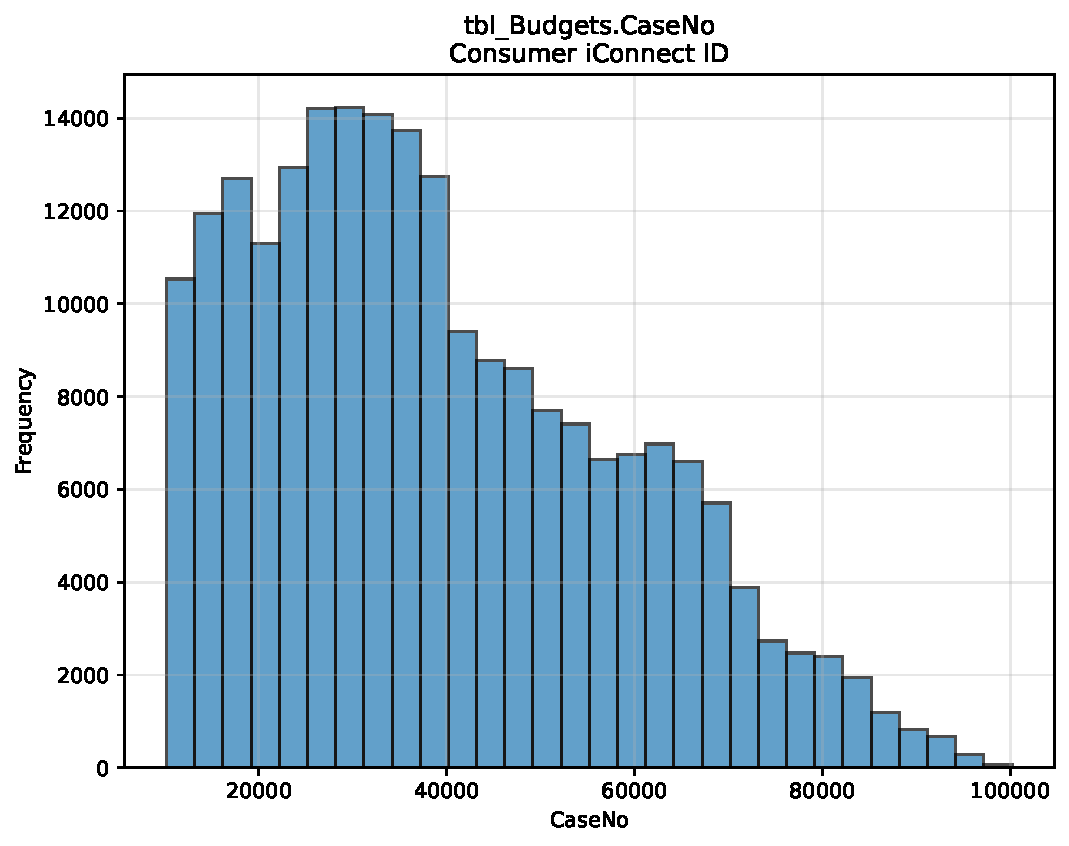
\includegraphics[width=\textwidth]{figures/dbo_tbl_Budgets_CaseNo.pdf}
\caption{Distribution of CaseNo in tbl\_Budgets}
\end{figure}\newpage

\subsection{tbl\_Budgets.BudgetID}

\begin{figure}[htbp]
\centering
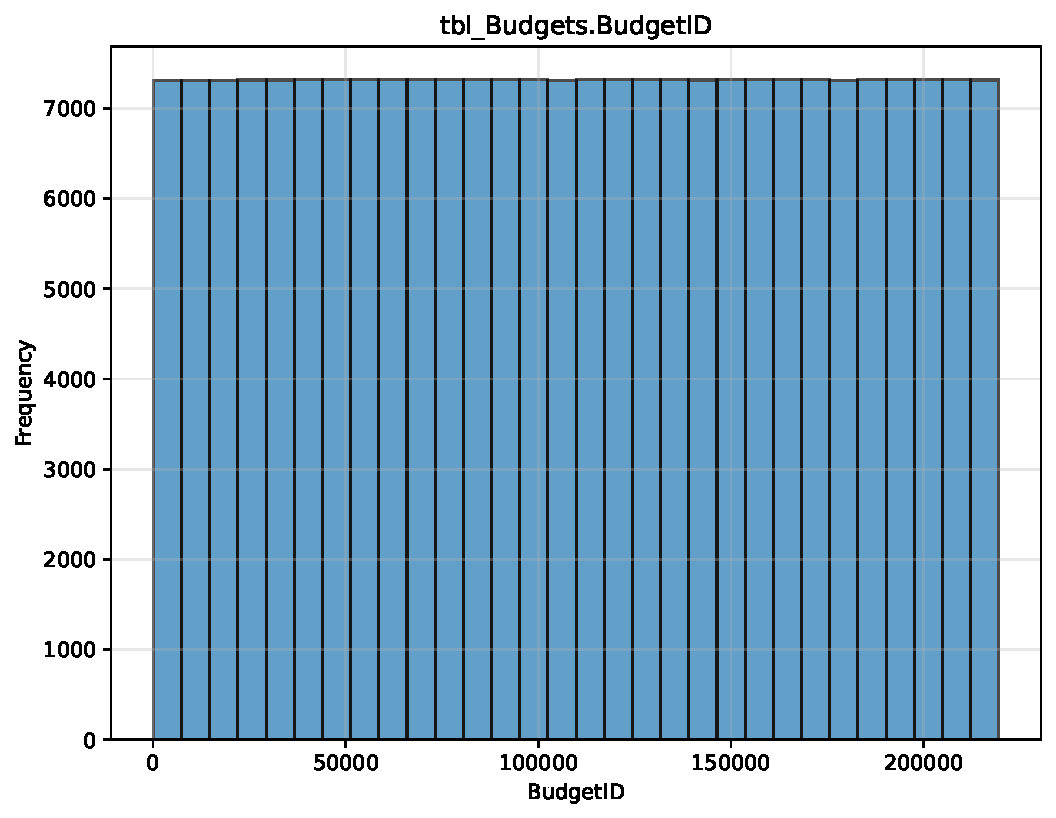
\includegraphics[width=\textwidth]{figures/dbo_tbl_Budgets_BudgetID.pdf}
\caption{Distribution of BudgetID in tbl\_Budgets}
\end{figure}\newpage

\subsection{tbl\_Budgets.ApprovedBy}

\begin{figure}[htbp]
\centering
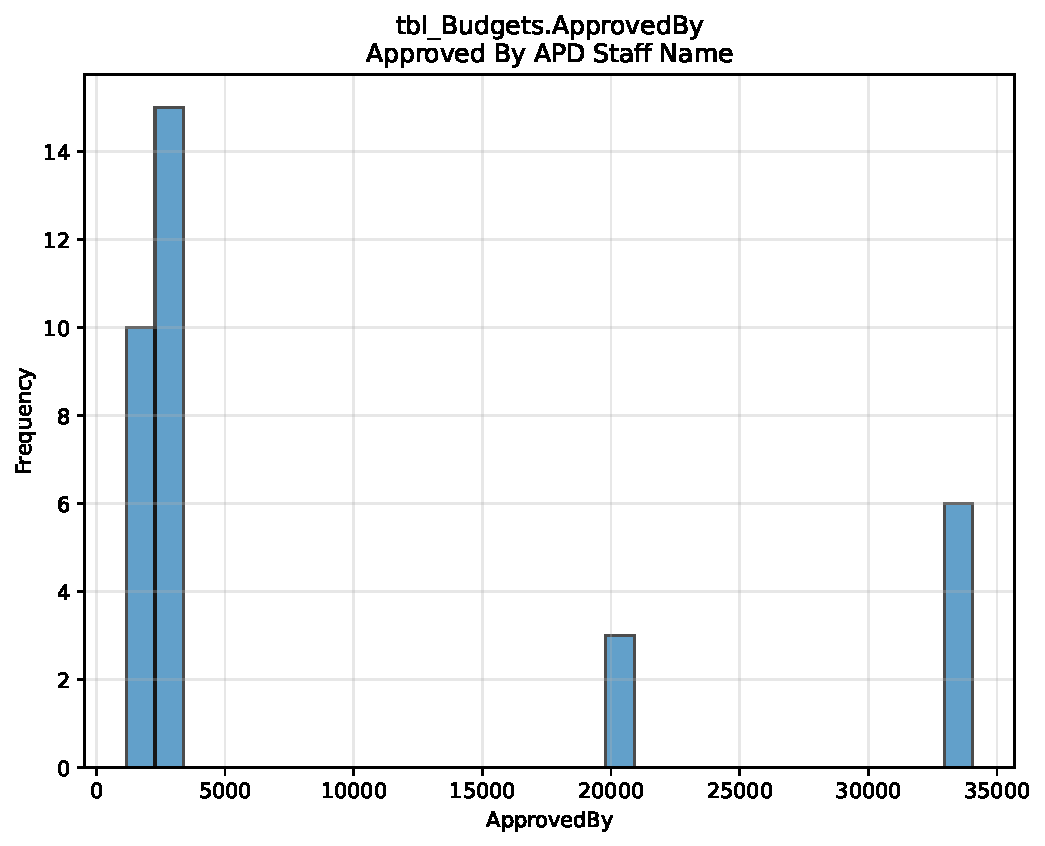
\includegraphics[width=\textwidth]{figures/dbo_tbl_Budgets_ApprovedBy.pdf}
\caption{Distribution of ApprovedBy in tbl\_Budgets}
\end{figure}\newpage

\subsection{tbl\_Budgets.BudgetAmount}

\begin{figure}[htbp]
\centering
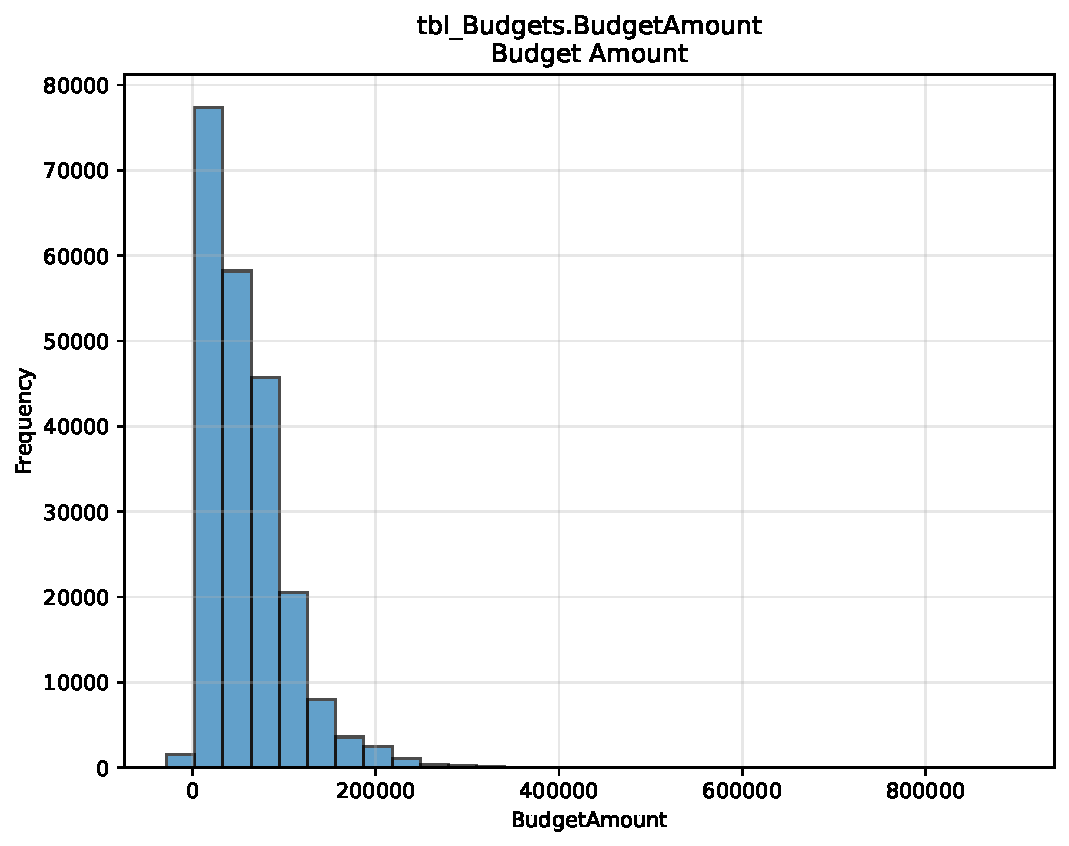
\includegraphics[width=\textwidth]{figures/dbo_tbl_Budgets_BudgetAmount.pdf}
\caption{Distribution of BudgetAmount in tbl\_Budgets}
\end{figure}\newpage

\subsection{tbl\_Budgets.AnnualizedAmount}

\begin{figure}[htbp]
\centering
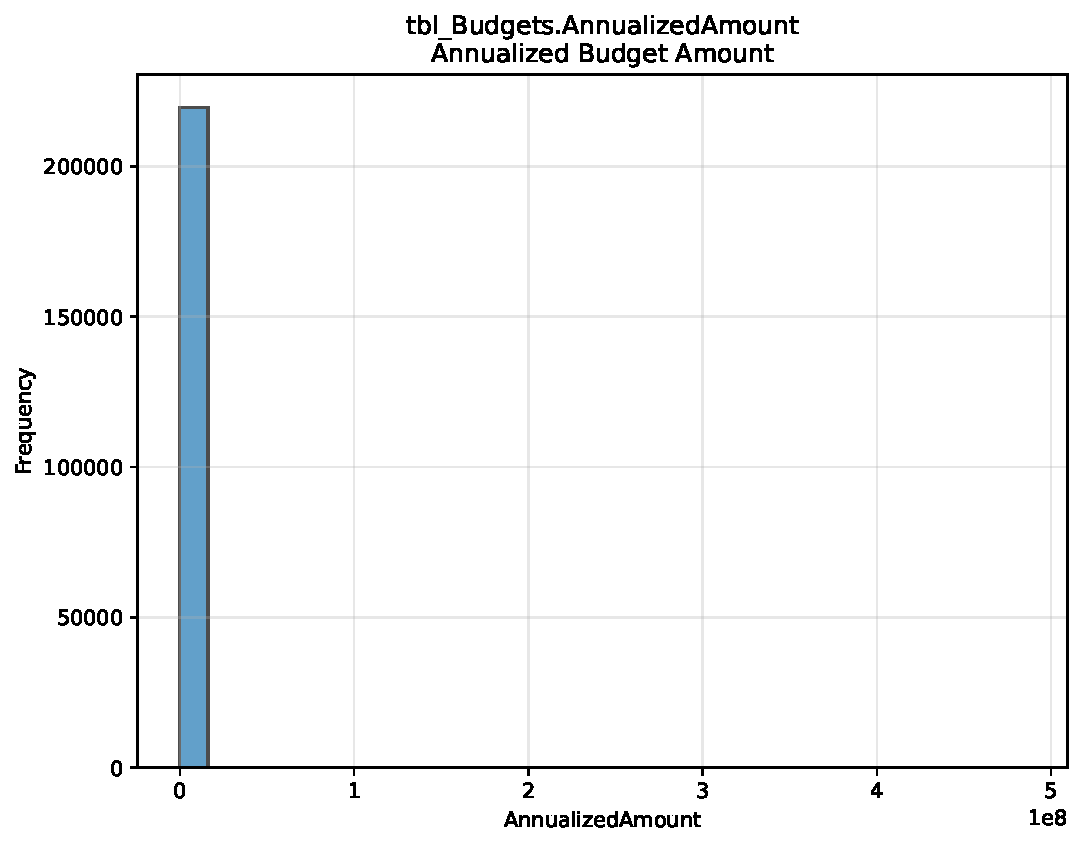
\includegraphics[width=\textwidth]{figures/dbo_tbl_Budgets_AnnualizedAmount.pdf}
\caption{Distribution of AnnualizedAmount in tbl\_Budgets}
\end{figure}\newpage

\subsection{tbl\_Budgets.AmountEncumbered}

\begin{figure}[htbp]
\centering
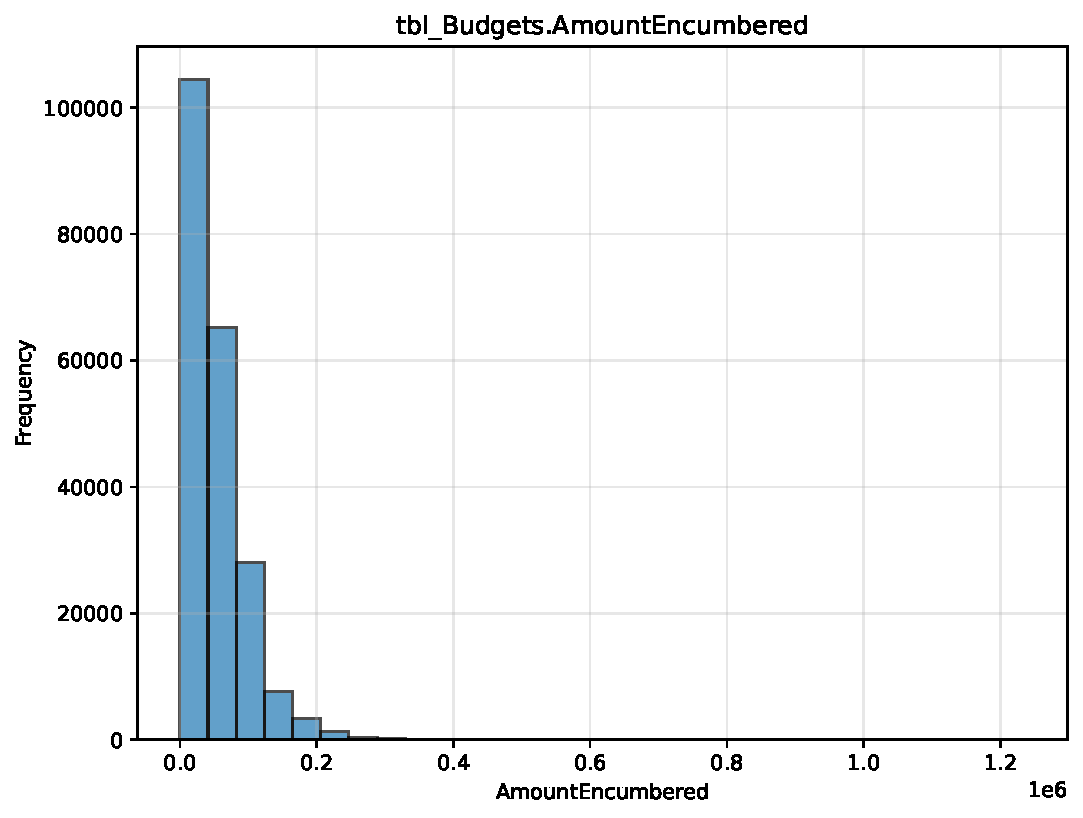
\includegraphics[width=\textwidth]{figures/dbo_tbl_Budgets_AmountEncumbered.pdf}
\caption{Distribution of AmountEncumbered in tbl\_Budgets}
\end{figure}\newpage

\subsection{tbl\_Budgets.AmountUnauthorized}

\begin{figure}[htbp]
\centering
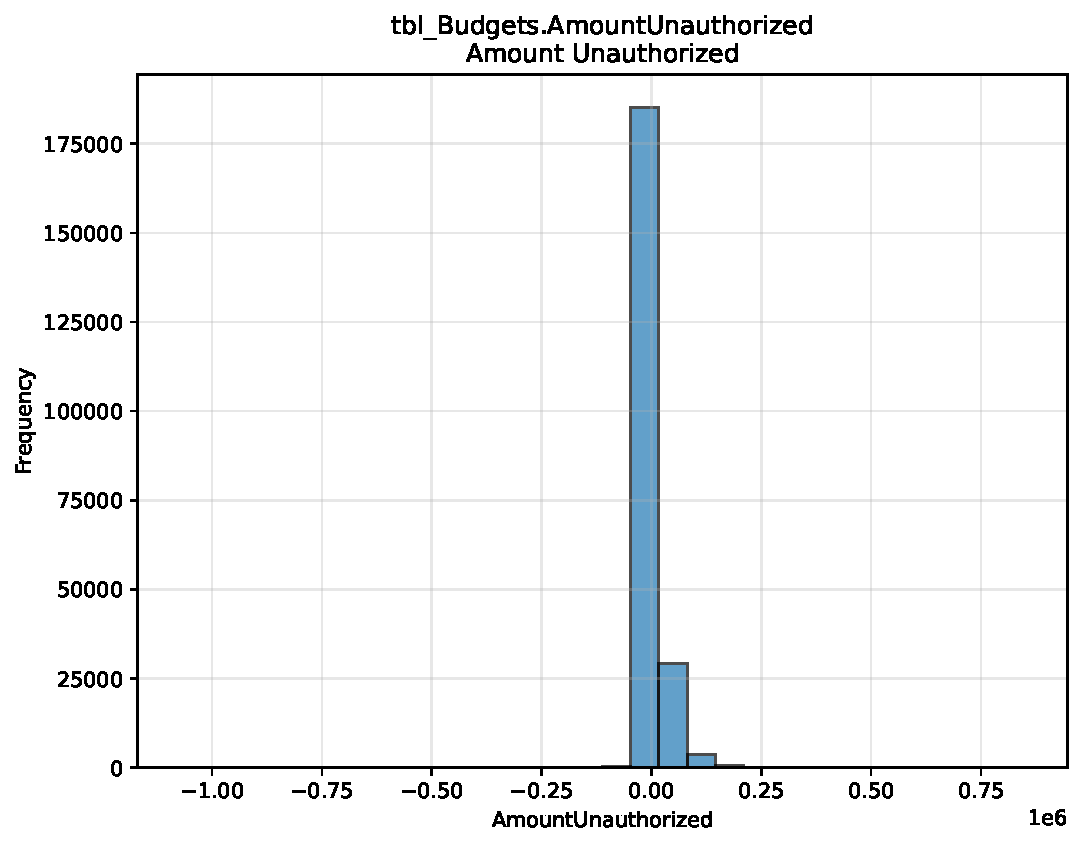
\includegraphics[width=\textwidth]{figures/dbo_tbl_Budgets_AmountUnauthorized.pdf}
\caption{Distribution of AmountUnauthorized in tbl\_Budgets}
\end{figure}\newpage

\subsection{tbl\_Budgets.PrioriBudgetAmount}

\begin{figure}[htbp]
\centering
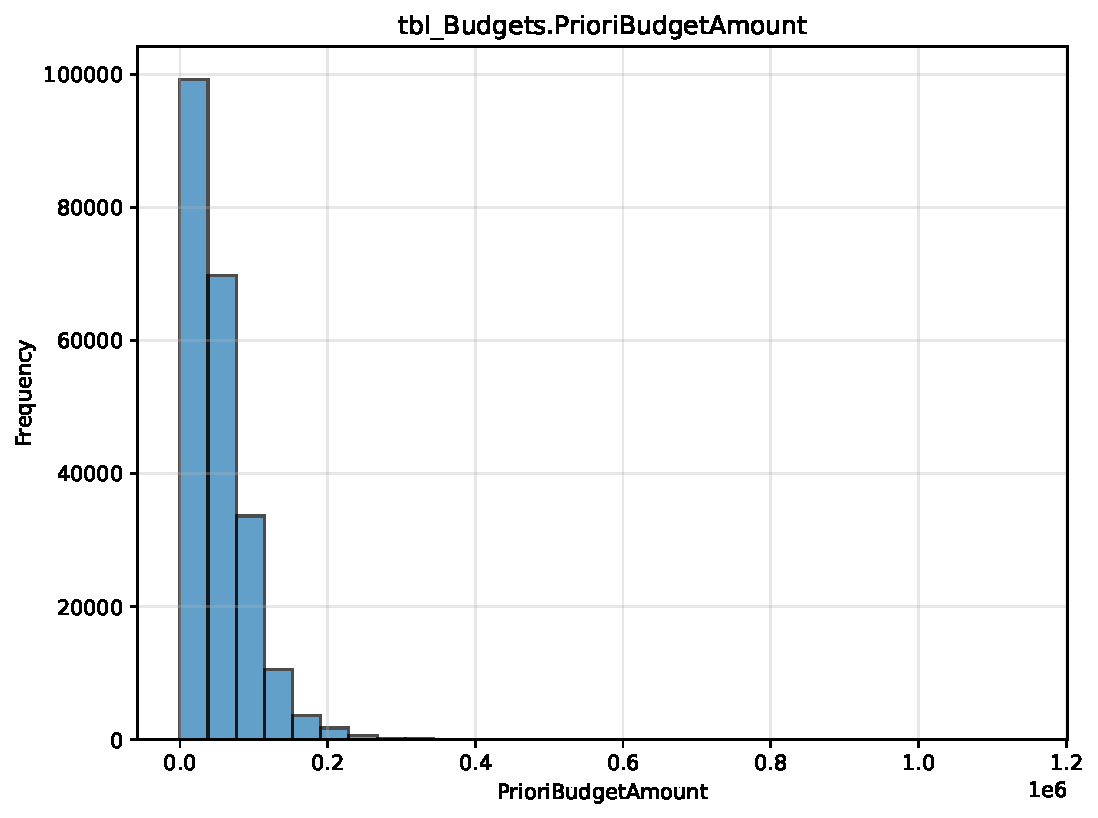
\includegraphics[width=\textwidth]{figures/dbo_tbl_Budgets_PrioriBudgetAmount.pdf}
\caption{Distribution of PrioriBudgetAmount in tbl\_Budgets}
\end{figure}\newpage

\subsection{tbl\_Claims\_MMIS.CaseNo}

\begin{figure}[htbp]
\centering
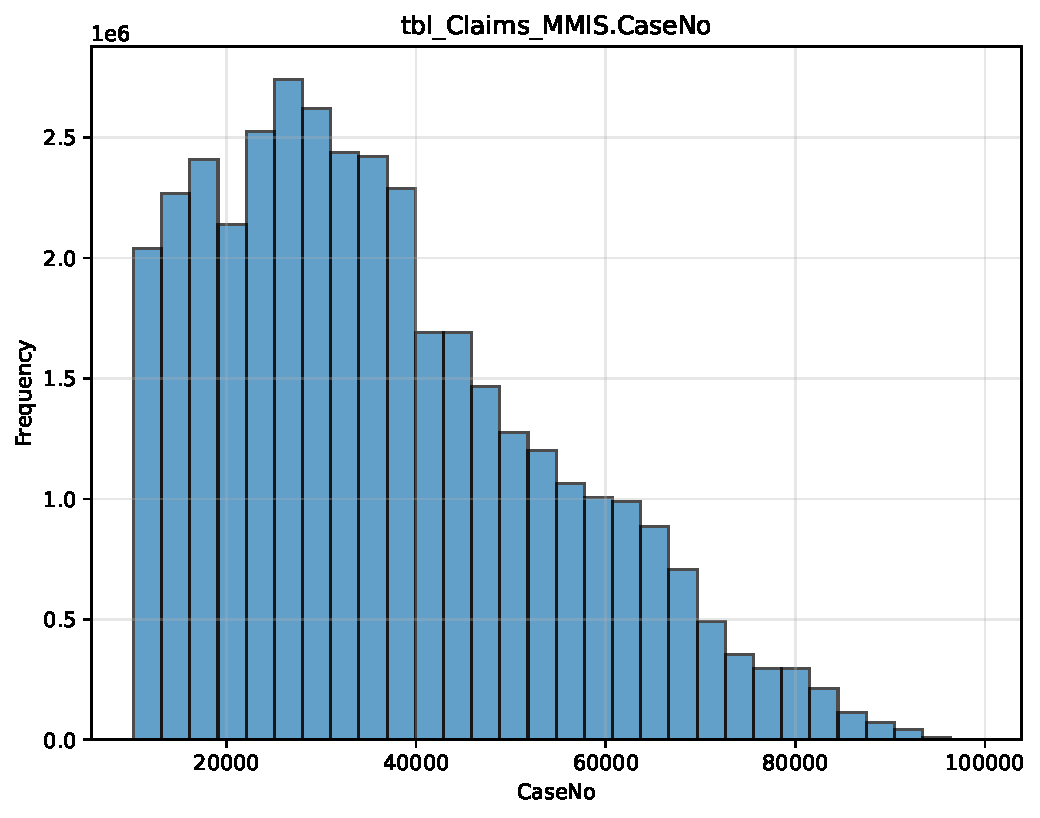
\includegraphics[width=\textwidth]{figures/dbo_tbl_Claims_MMIS_CaseNo.pdf}
\caption{Distribution of CaseNo in tbl\_Claims\_MMIS}
\end{figure}\newpage

\subsection{tbl\_Claims\_MMIS.Units}

\begin{figure}[htbp]
\centering
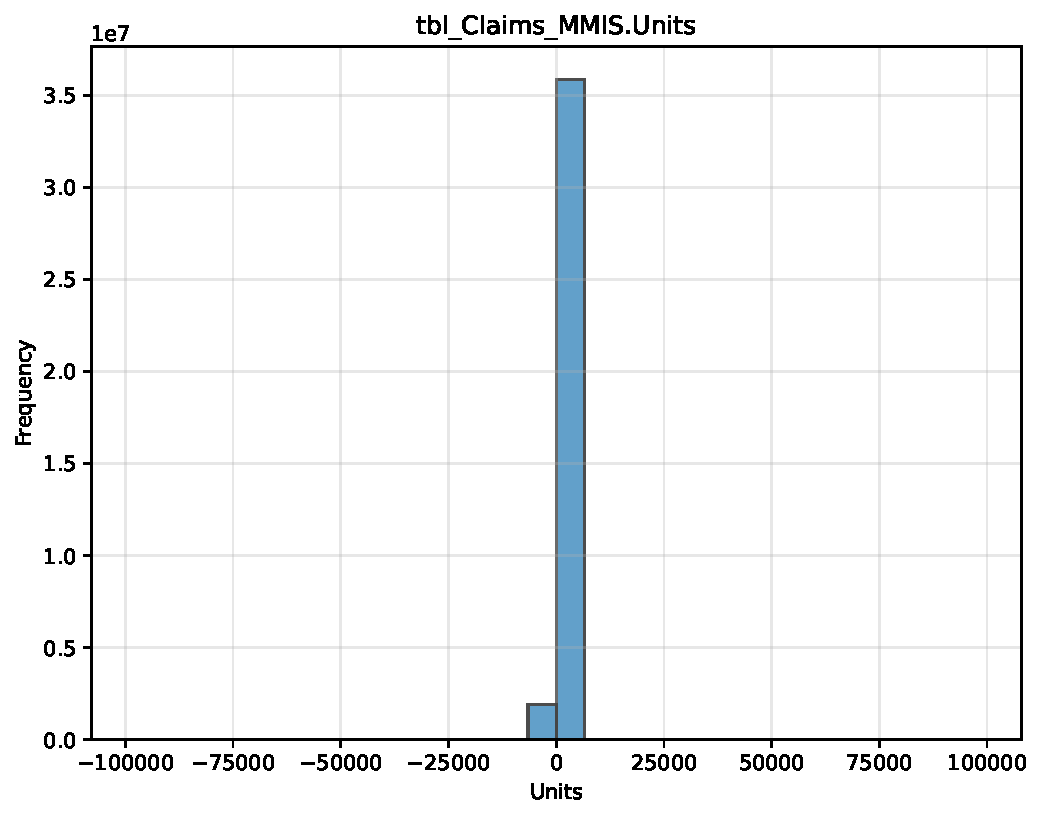
\includegraphics[width=\textwidth]{figures/dbo_tbl_Claims_MMIS_Units.pdf}
\caption{Distribution of Units in tbl\_Claims\_MMIS}
\end{figure}\newpage

\subsection{tbl\_Claims\_MMIS.BilledAmt}

\begin{figure}[htbp]
\centering
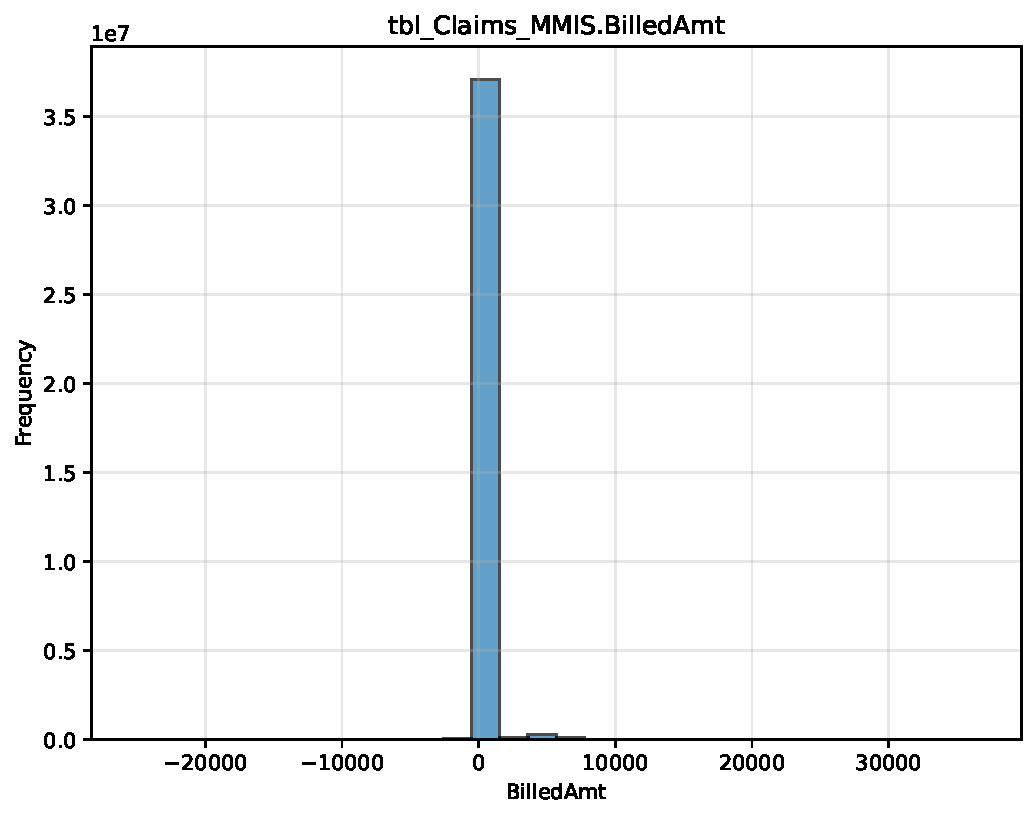
\includegraphics[width=\textwidth]{figures/dbo_tbl_Claims_MMIS_BilledAmt.pdf}
\caption{Distribution of BilledAmt in tbl\_Claims\_MMIS}
\end{figure}\newpage

\subsection{tbl\_Claims\_MMIS.PaidAmt}

\begin{figure}[htbp]
\centering
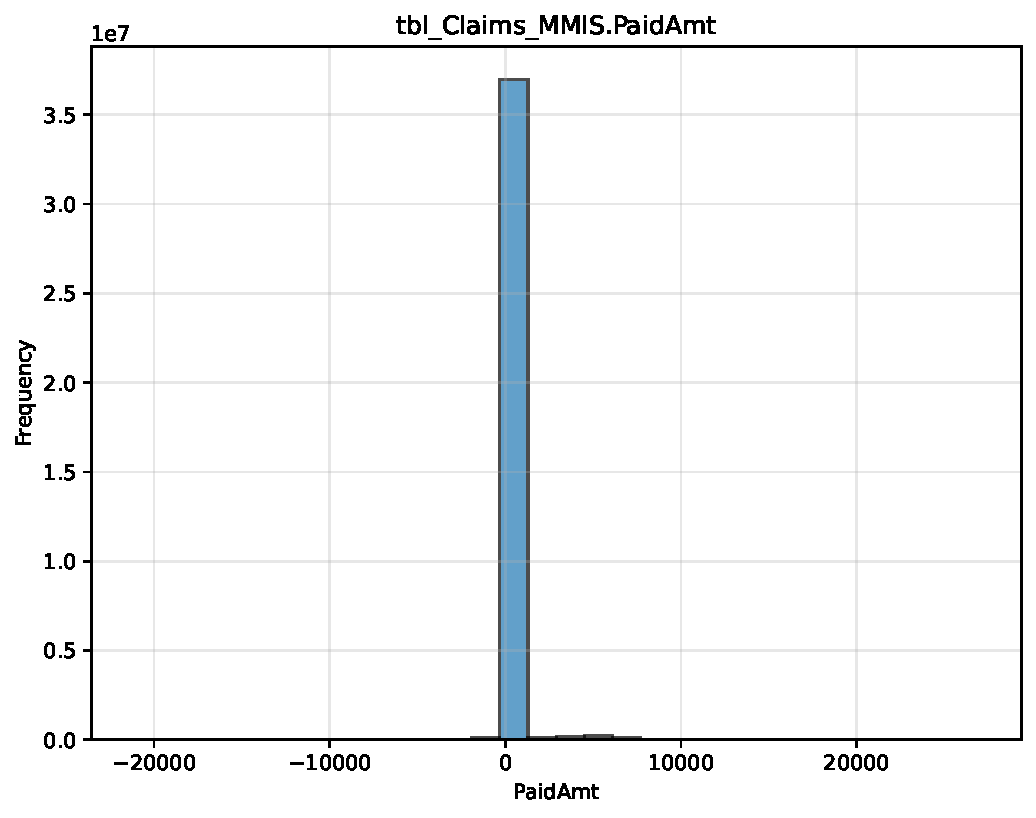
\includegraphics[width=\textwidth]{figures/dbo_tbl_Claims_MMIS_PaidAmt.pdf}
\caption{Distribution of PaidAmt in tbl\_Claims\_MMIS}
\end{figure}\newpage

\subsection{tbl\_Claims\_MMIS.Id}

\begin{figure}[htbp]
\centering
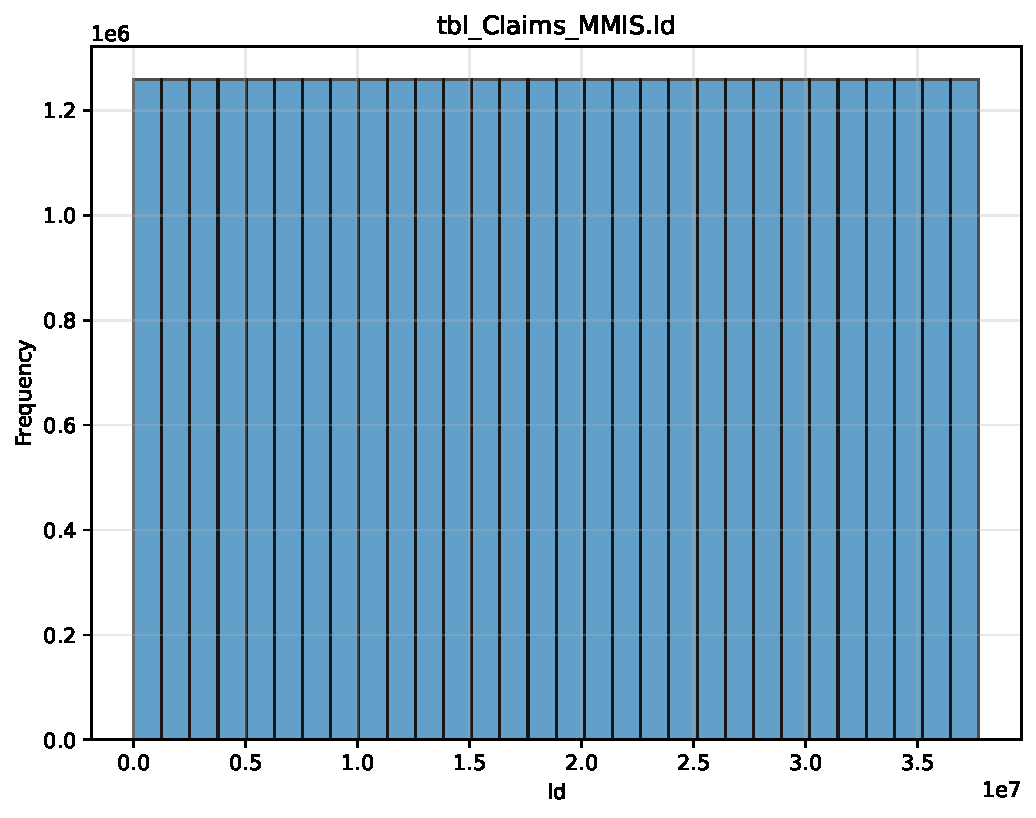
\includegraphics[width=\textwidth]{figures/dbo_tbl_Claims_MMIS_Id.pdf}
\caption{Distribution of Id in tbl\_Claims\_MMIS}
\end{figure}\newpage

\subsection{tbl\_ConsumerContacts.CONTACTID}

\begin{figure}[htbp]
\centering
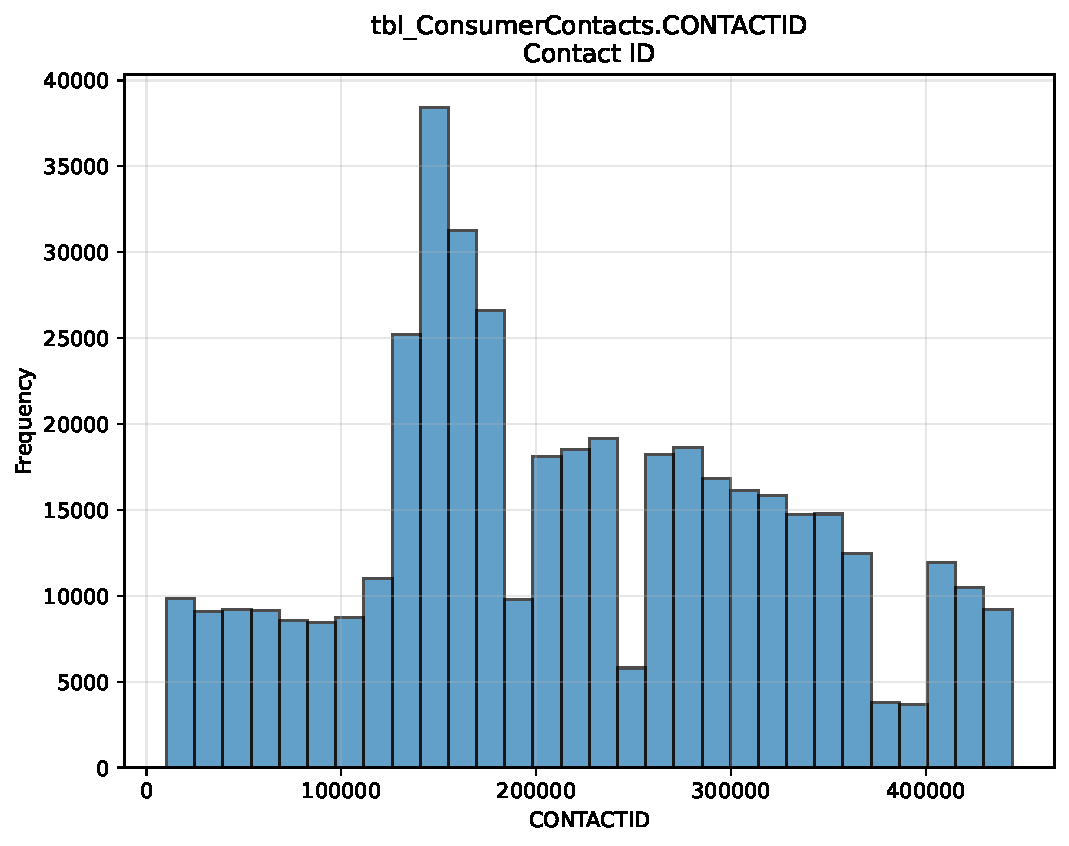
\includegraphics[width=\textwidth]{figures/dbo_tbl_ConsumerContacts_CONTACTID.pdf}
\caption{Distribution of CONTACTID in tbl\_ConsumerContacts}
\end{figure}\newpage

\subsection{tbl\_ConsumerContacts.CASENO}

\begin{figure}[htbp]
\centering
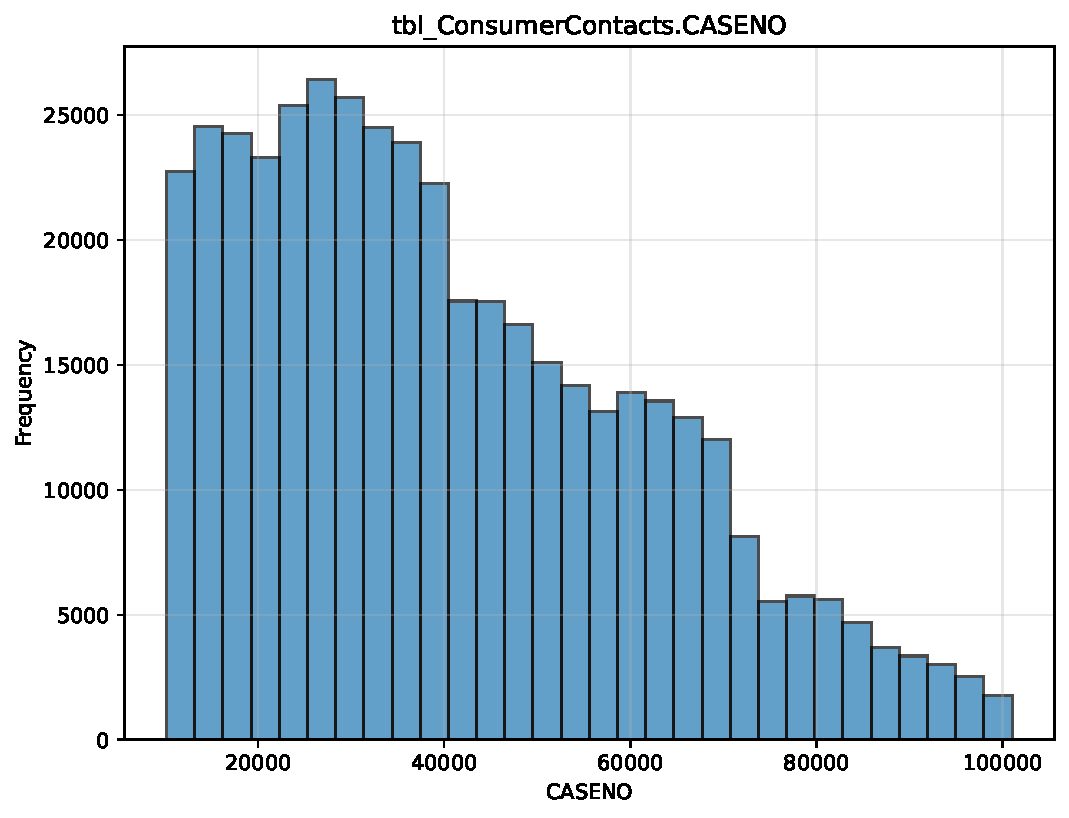
\includegraphics[width=\textwidth]{figures/dbo_tbl_ConsumerContacts_CASENO.pdf}
\caption{Distribution of CASENO in tbl\_ConsumerContacts}
\end{figure}\newpage

\subsection{tbl\_ConsumerContacts.Active}

\begin{figure}[htbp]
\centering
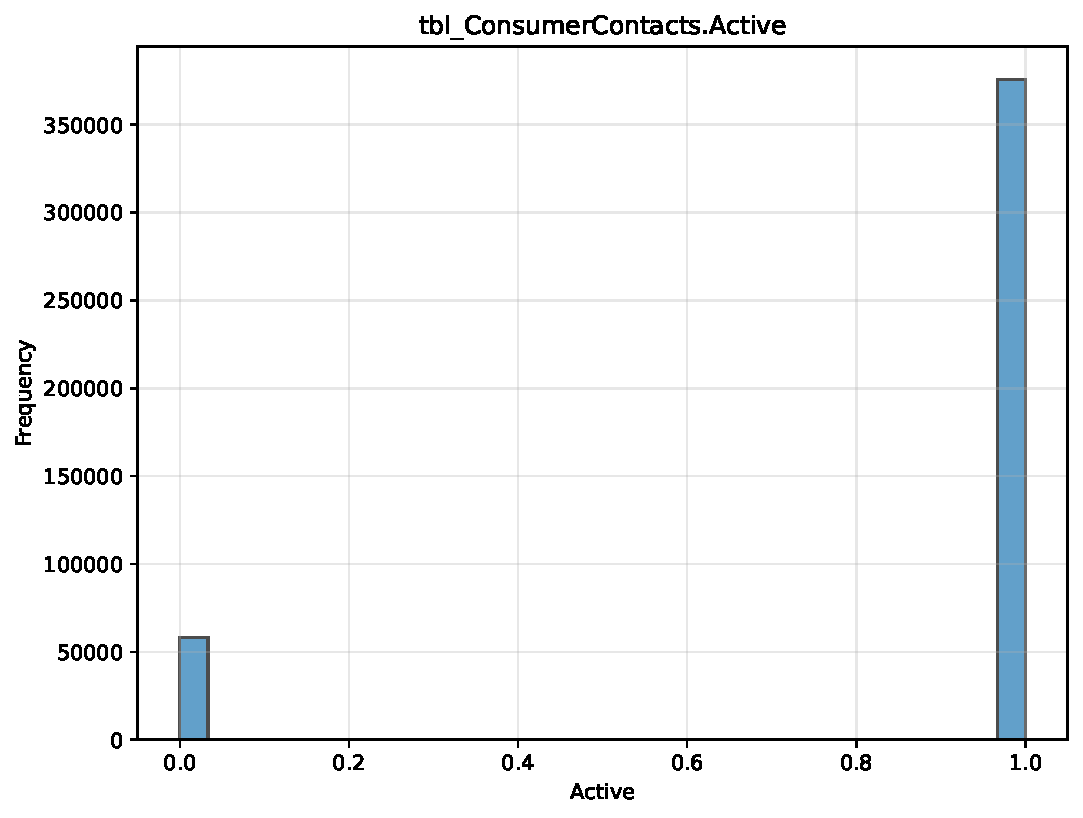
\includegraphics[width=\textwidth]{figures/dbo_tbl_ConsumerContacts_Active.pdf}
\caption{Distribution of Active in tbl\_ConsumerContacts}
\end{figure}\newpage

\subsection{tbl\_ConsumerContacts.RECID}

\begin{figure}[htbp]
\centering
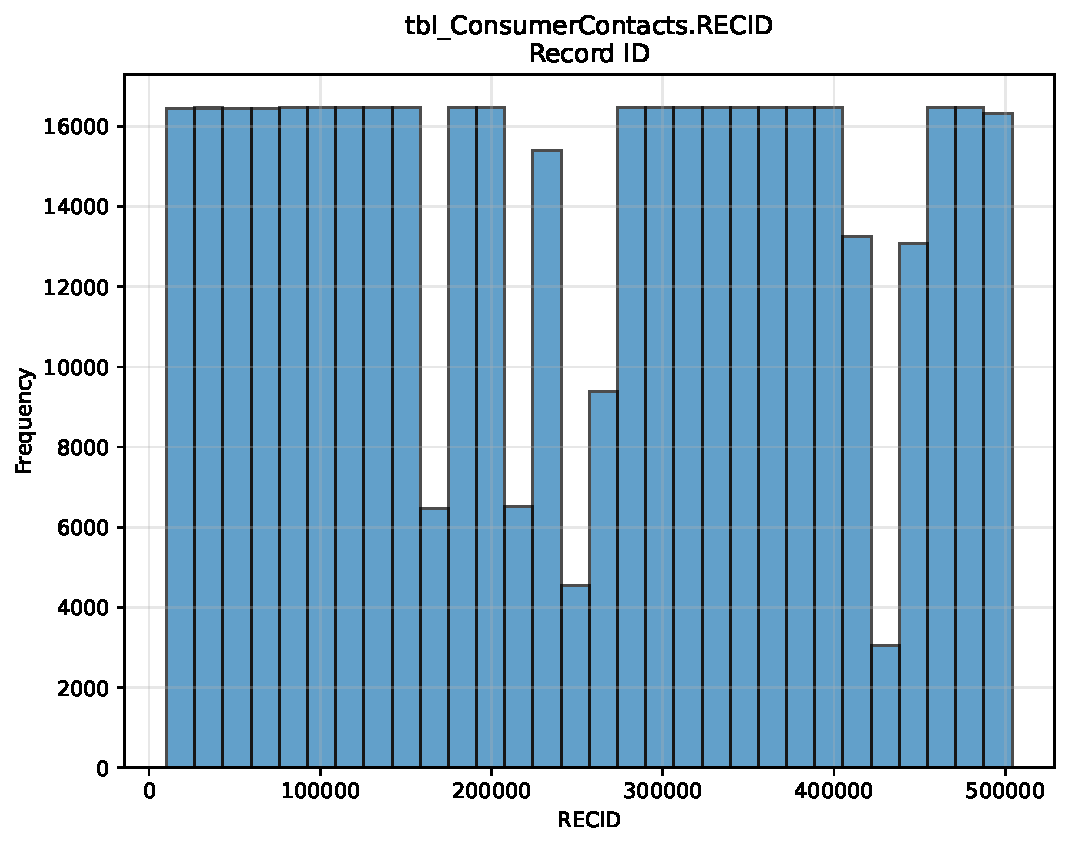
\includegraphics[width=\textwidth]{figures/dbo_tbl_ConsumerContacts_RECID.pdf}
\caption{Distribution of RECID in tbl\_ConsumerContacts}
\end{figure}\newpage

\subsection{tbl\_Consumers.CASENO}

\begin{figure}[htbp]
\centering
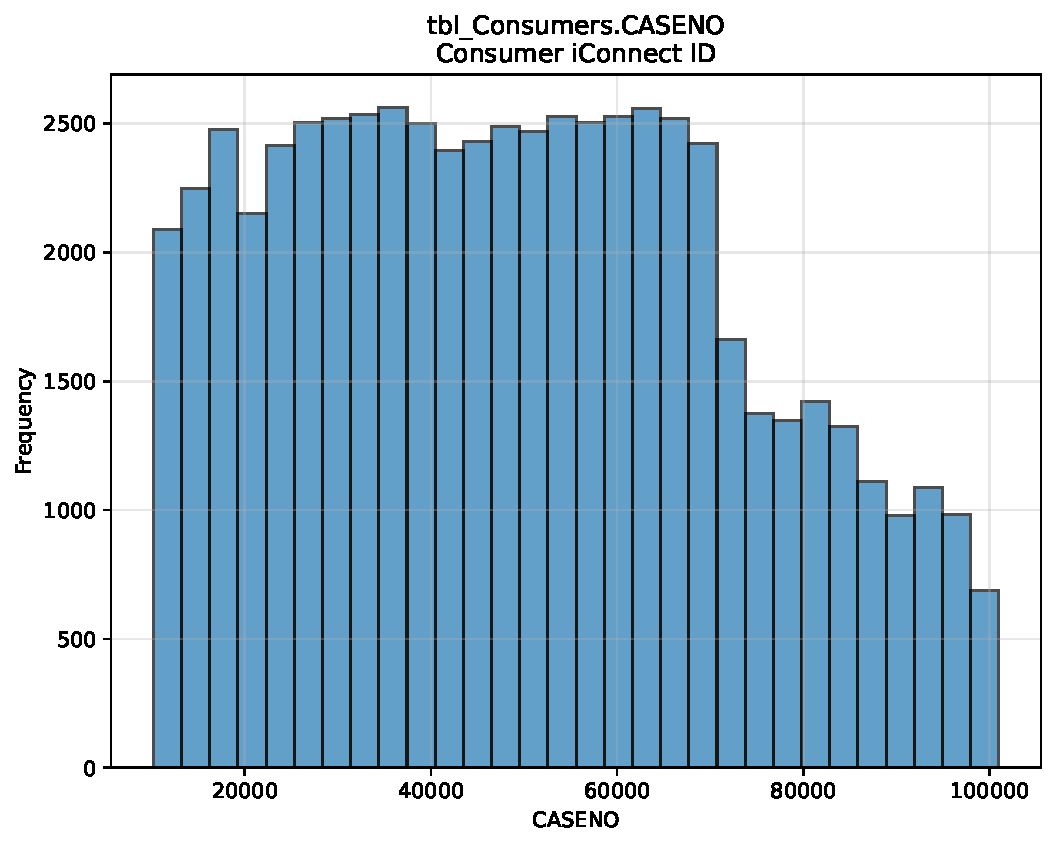
\includegraphics[width=\textwidth]{figures/dbo_tbl_Consumers_CASENO.pdf}
\caption{Distribution of CASENO in tbl\_Consumers}
\end{figure}\newpage

\subsection{tbl\_Consumers.CBCFlag}

\begin{figure}[htbp]
\centering
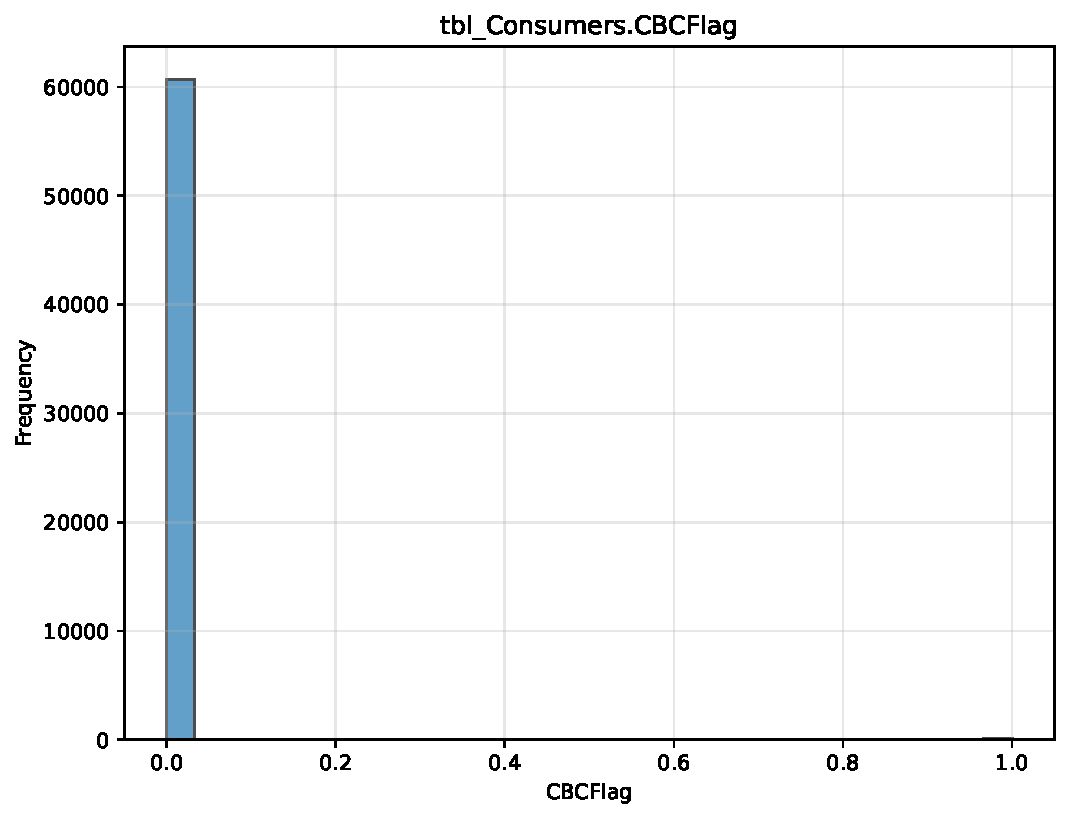
\includegraphics[width=\textwidth]{figures/dbo_tbl_Consumers_CBCFlag.pdf}
\caption{Distribution of CBCFlag in tbl\_Consumers}
\end{figure}\newpage

\subsection{tbl\_Consumers.ANNUALINCOME}

\begin{figure}[htbp]
\centering
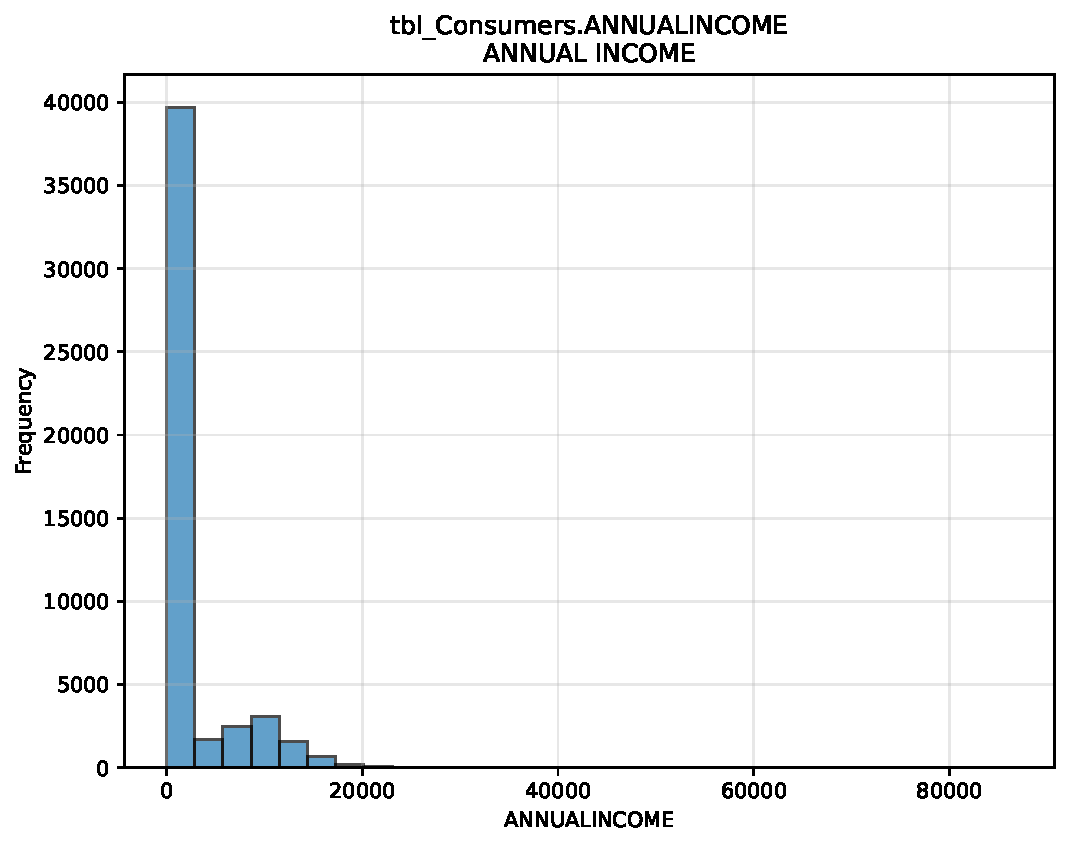
\includegraphics[width=\textwidth]{figures/dbo_tbl_Consumers_ANNUALINCOME.pdf}
\caption{Distribution of ANNUALINCOME in tbl\_Consumers}
\end{figure}\newpage

\subsection{tbl\_Consumers.OPENID}

\begin{figure}[htbp]
\centering
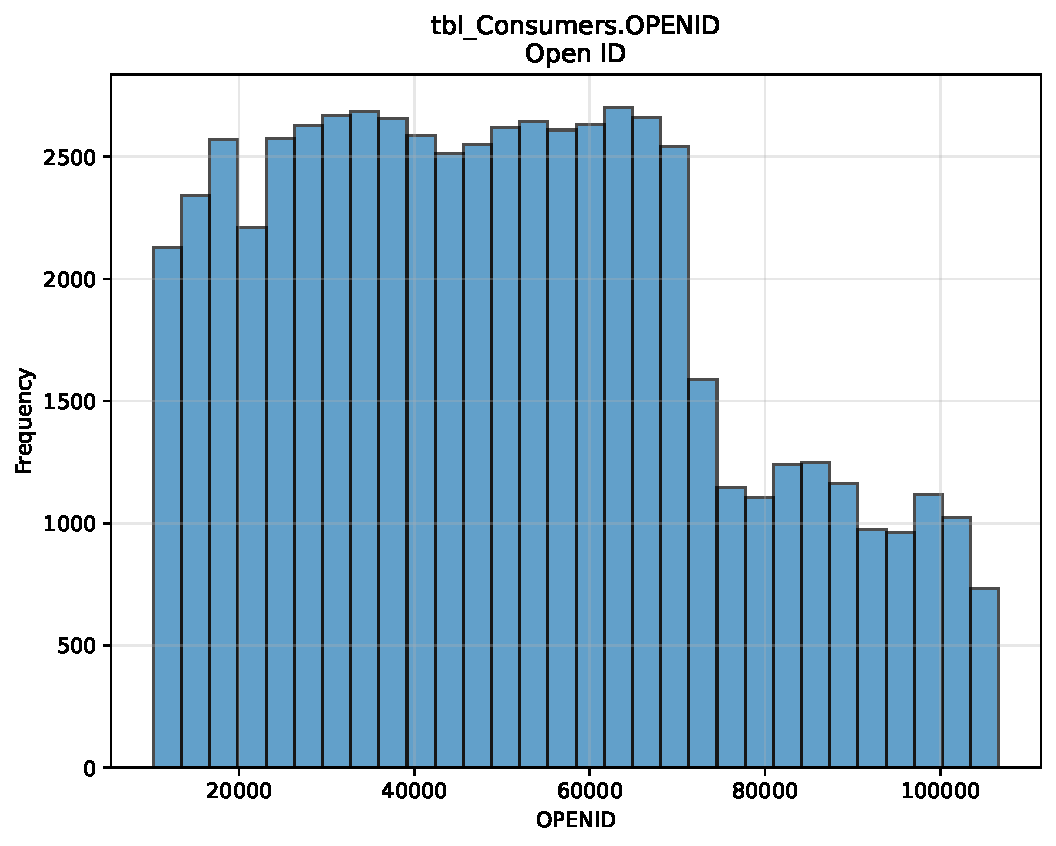
\includegraphics[width=\textwidth]{figures/dbo_tbl_Consumers_OPENID.pdf}
\caption{Distribution of OPENID in tbl\_Consumers}
\end{figure}\newpage

\subsection{tbl\_Consumers.PRIMARYWORKERID}

\begin{figure}[htbp]
\centering
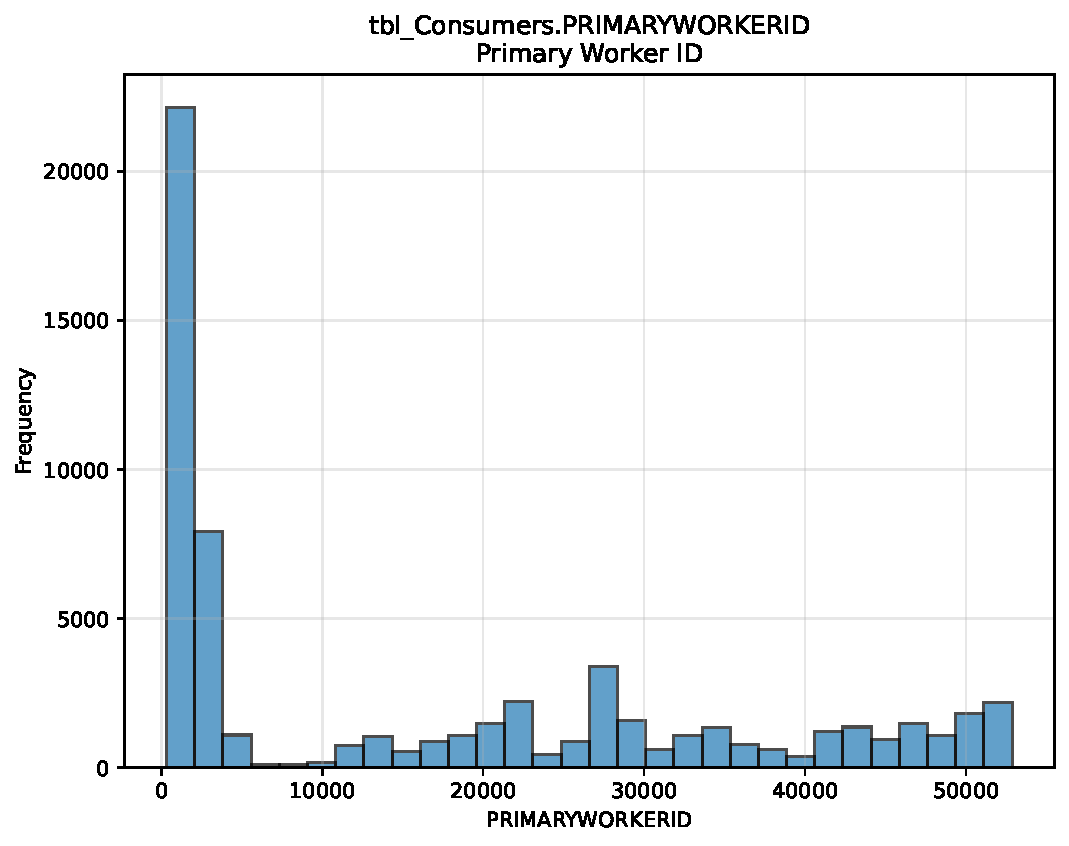
\includegraphics[width=\textwidth]{figures/dbo_tbl_Consumers_PRIMARYWORKERID.pdf}
\caption{Distribution of PRIMARYWORKERID in tbl\_Consumers}
\end{figure}\newpage

\subsection{tbl\_Consumers.SECONDWORKERID}

\begin{figure}[htbp]
\centering
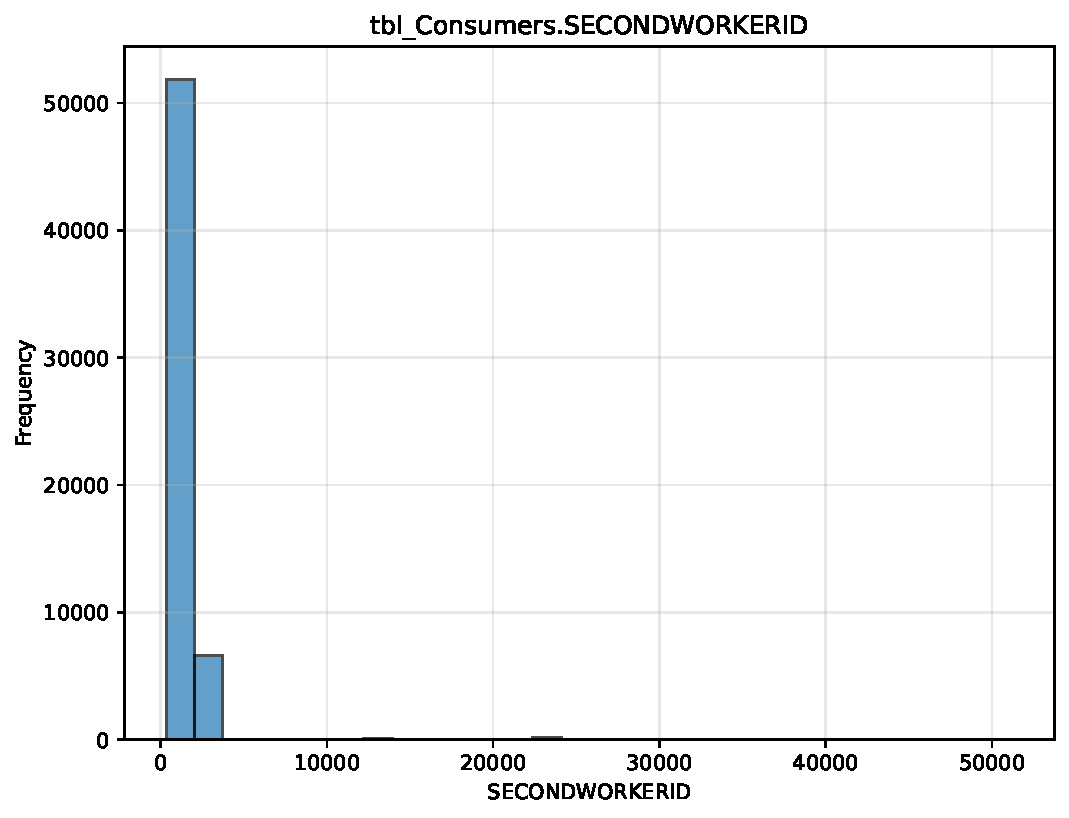
\includegraphics[width=\textwidth]{figures/dbo_tbl_Consumers_SECONDWORKERID.pdf}
\caption{Distribution of SECONDWORKERID in tbl\_Consumers}
\end{figure}\newpage

\subsection{tbl\_Consumers.CONTACTID}

\begin{figure}[htbp]
\centering
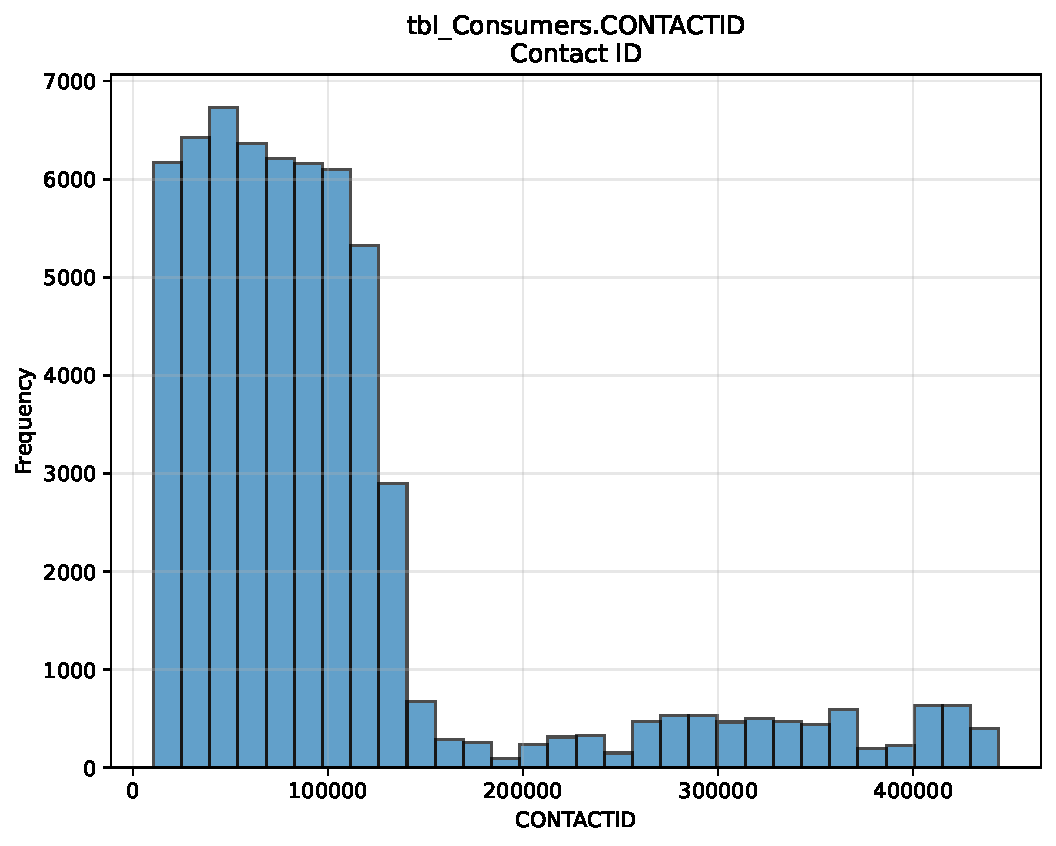
\includegraphics[width=\textwidth]{figures/dbo_tbl_Consumers_CONTACTID.pdf}
\caption{Distribution of CONTACTID in tbl\_Consumers}
\end{figure}\newpage

\subsection{tbl\_Consumers.Id}

\begin{figure}[htbp]
\centering
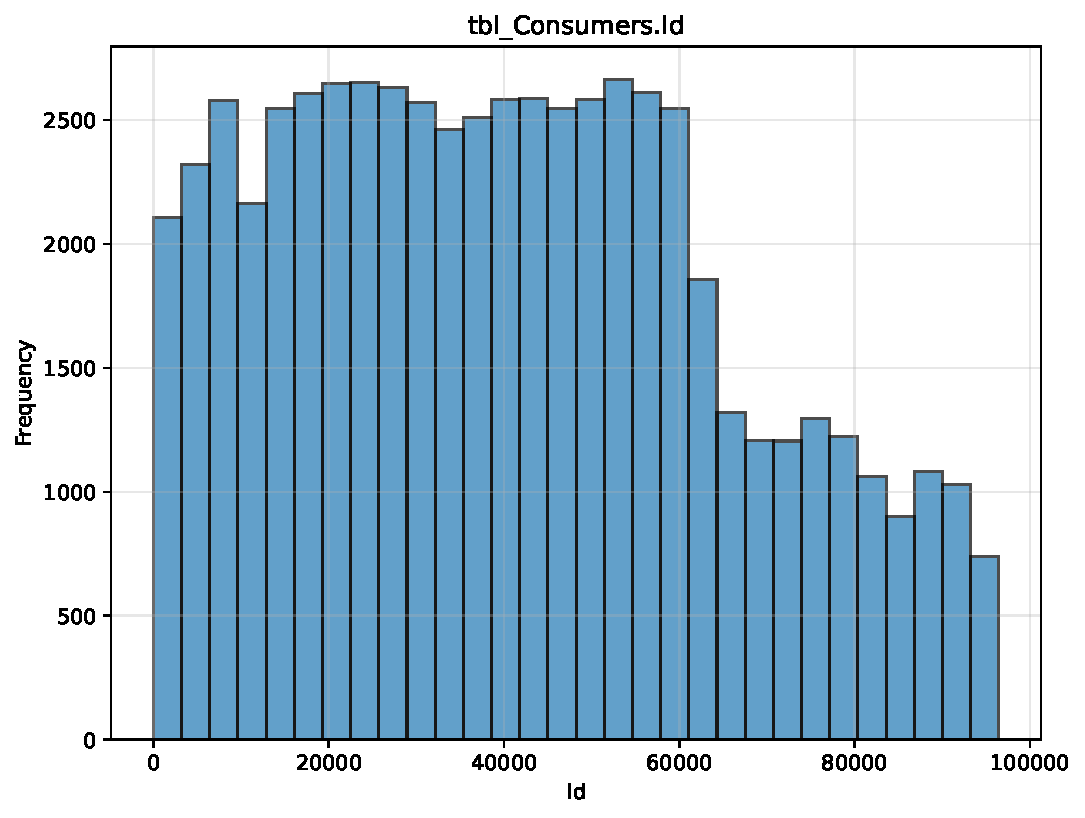
\includegraphics[width=\textwidth]{figures/dbo_tbl_Consumers_Id.pdf}
\caption{Distribution of Id in tbl\_Consumers}
\end{figure}\newpage

\subsection{tbl\_Diagnosis.CASENO}

\begin{figure}[htbp]
\centering
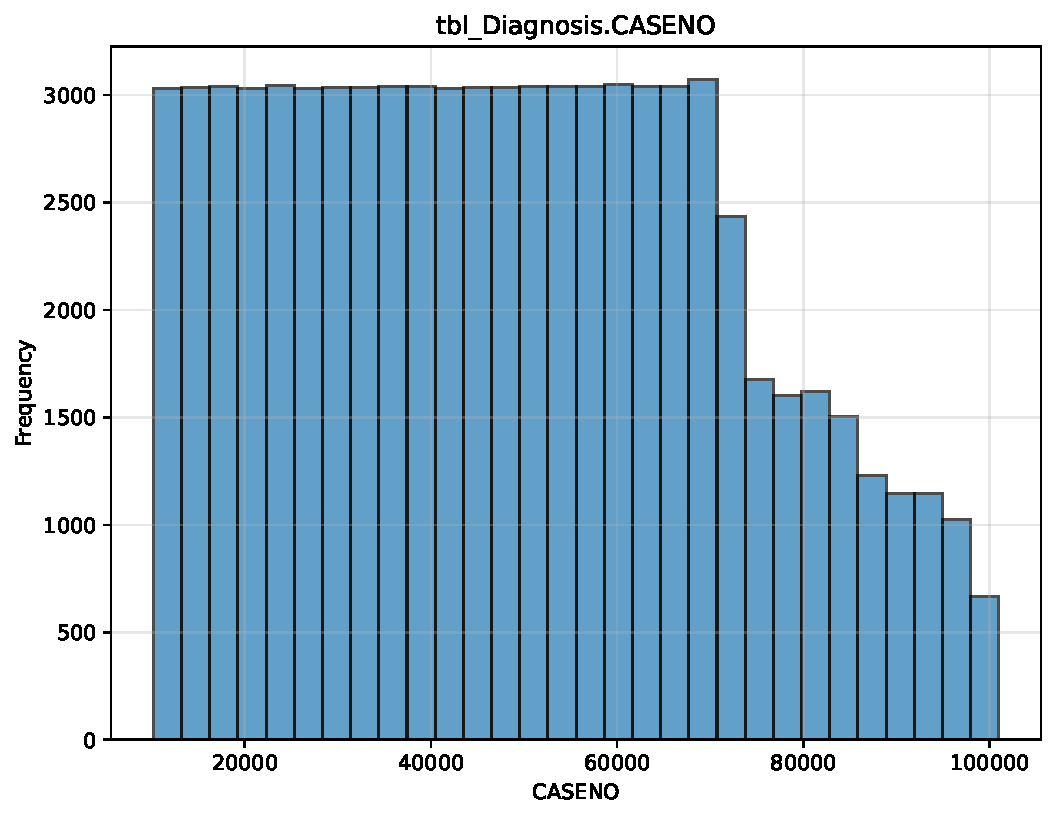
\includegraphics[width=\textwidth]{figures/dbo_tbl_Diagnosis_CASENO.pdf}
\caption{Distribution of CASENO in tbl\_Diagnosis}
\end{figure}\newpage

\subsection{tbl\_Diagnosis.DiagnosisID}

\begin{figure}[htbp]
\centering
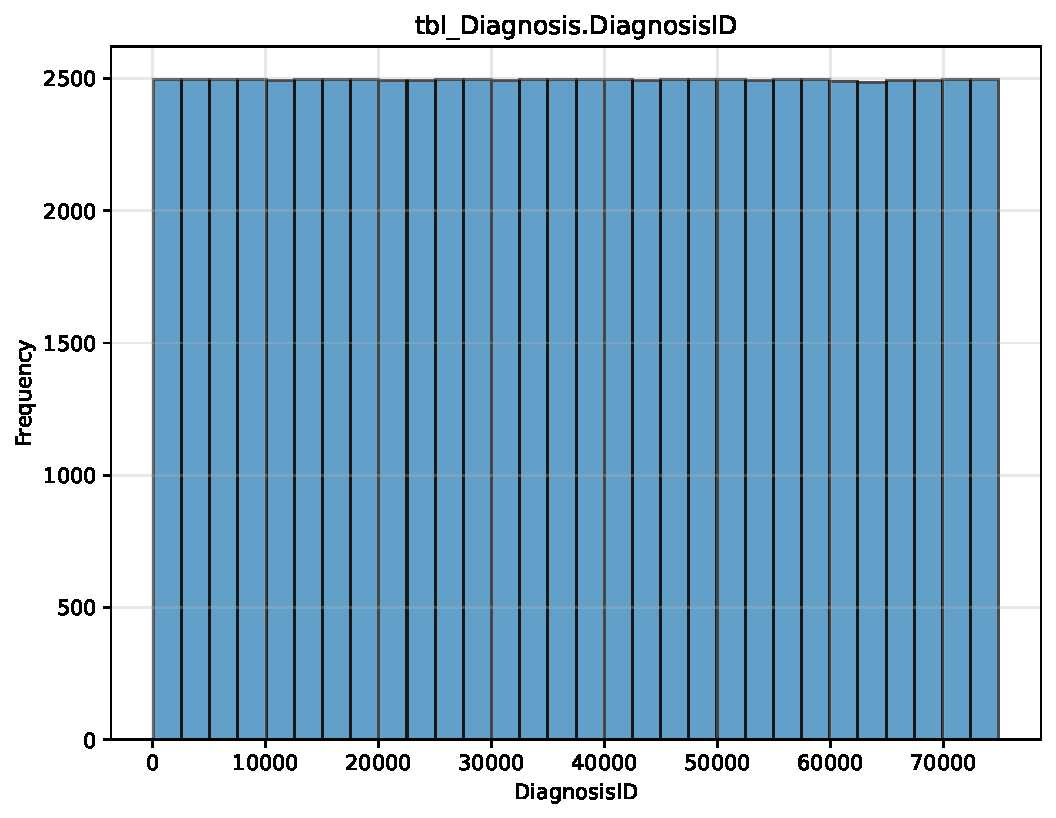
\includegraphics[width=\textwidth]{figures/dbo_tbl_Diagnosis_DiagnosisID.pdf}
\caption{Distribution of DiagnosisID in tbl\_Diagnosis}
\end{figure}\newpage

\subsection{tbl\_EZBudget.CASENO}

\begin{figure}[htbp]
\centering
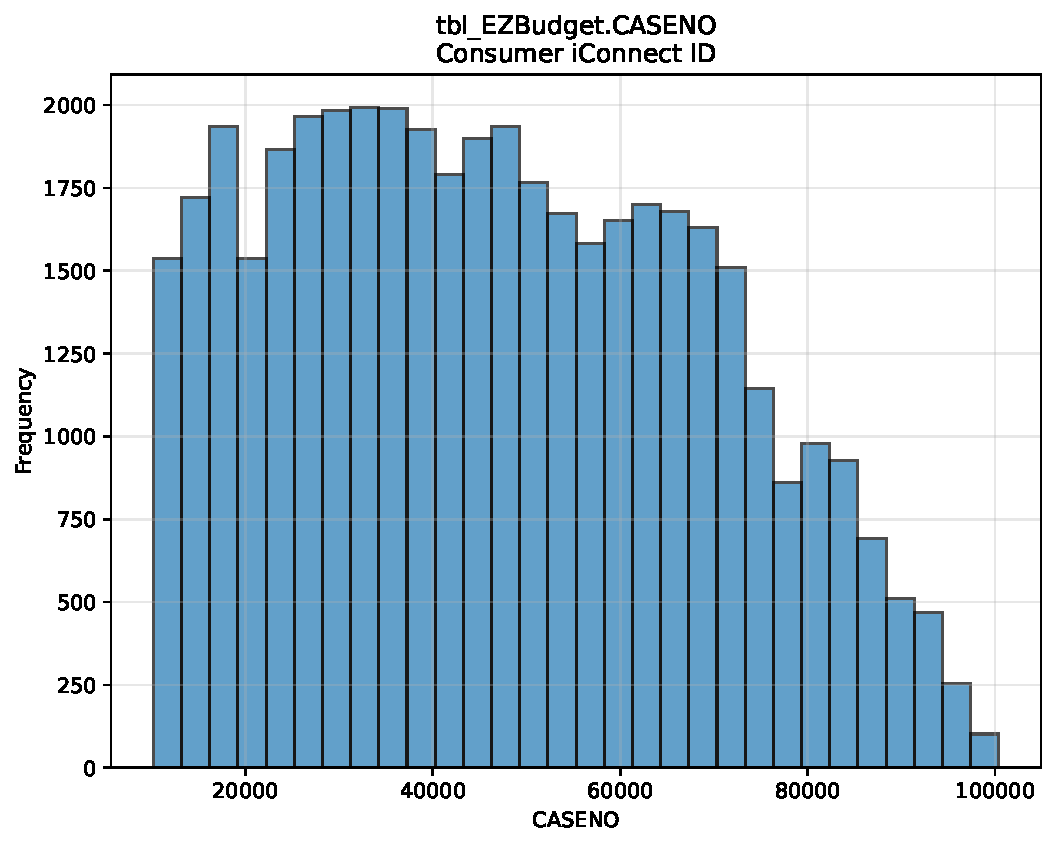
\includegraphics[width=\textwidth]{figures/dbo_tbl_EZBudget_CASENO.pdf}
\caption{Distribution of CASENO in tbl\_EZBudget}
\end{figure}\newpage

\subsection{tbl\_EZBudget.EZBudgetAssessId}

\begin{figure}[htbp]
\centering
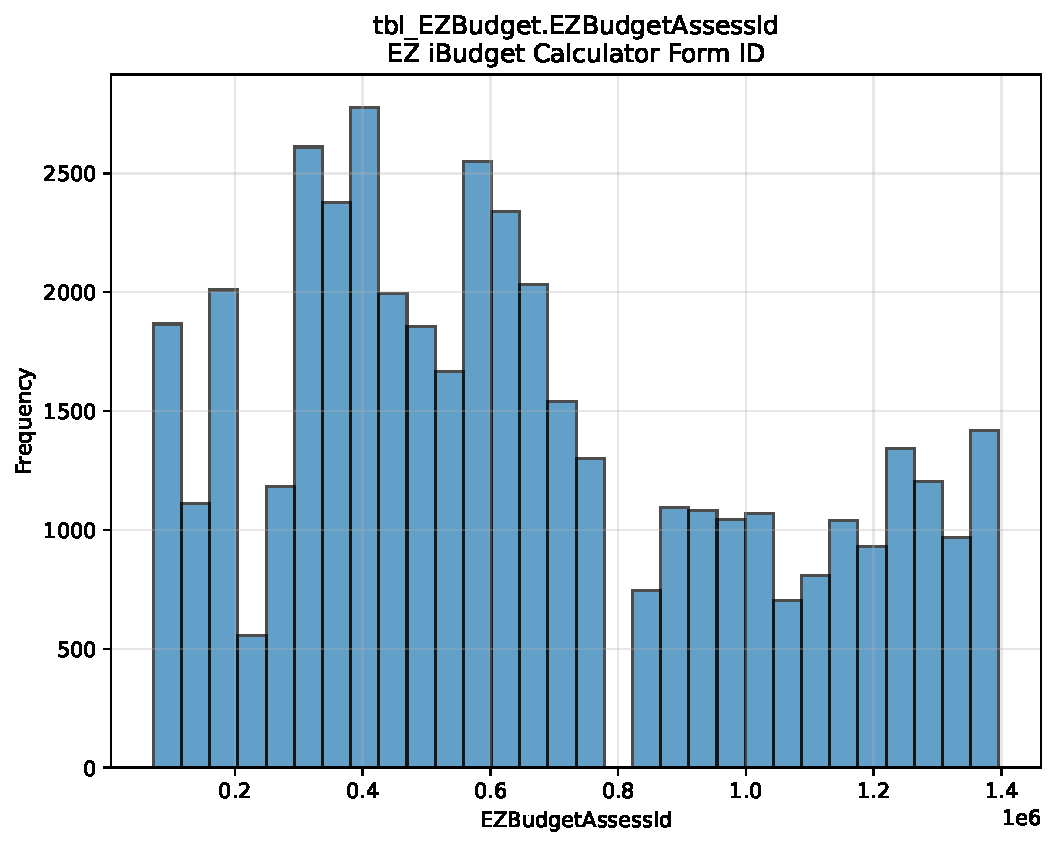
\includegraphics[width=\textwidth]{figures/dbo_tbl_EZBudget_EZBudgetAssessId.pdf}
\caption{Distribution of EZBudgetAssessId in tbl\_EZBudget}
\end{figure}\newpage

\subsection{tbl\_EZBudget.AlgorithmAmt}

\begin{figure}[htbp]
\centering
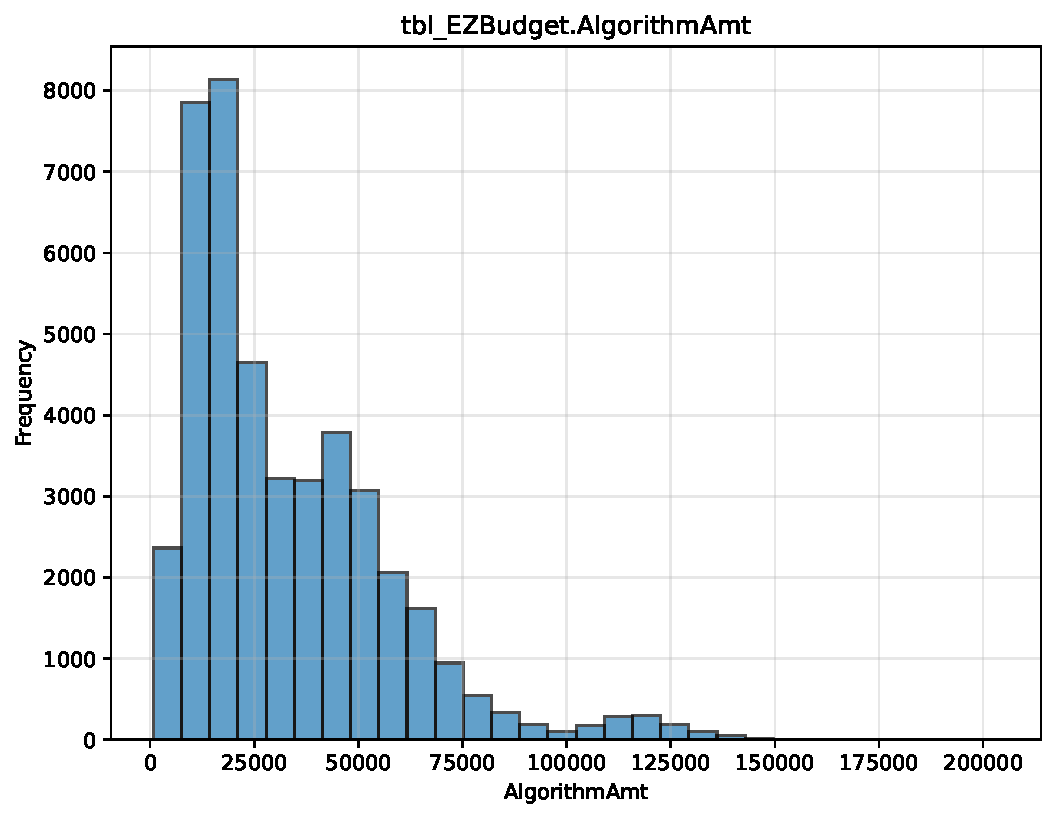
\includegraphics[width=\textwidth]{figures/dbo_tbl_EZBudget_AlgorithmAmt.pdf}
\caption{Distribution of AlgorithmAmt in tbl\_EZBudget}
\end{figure}\newpage

\subsection{tbl\_PlannedServices.CaseNo}

\begin{figure}[htbp]
\centering
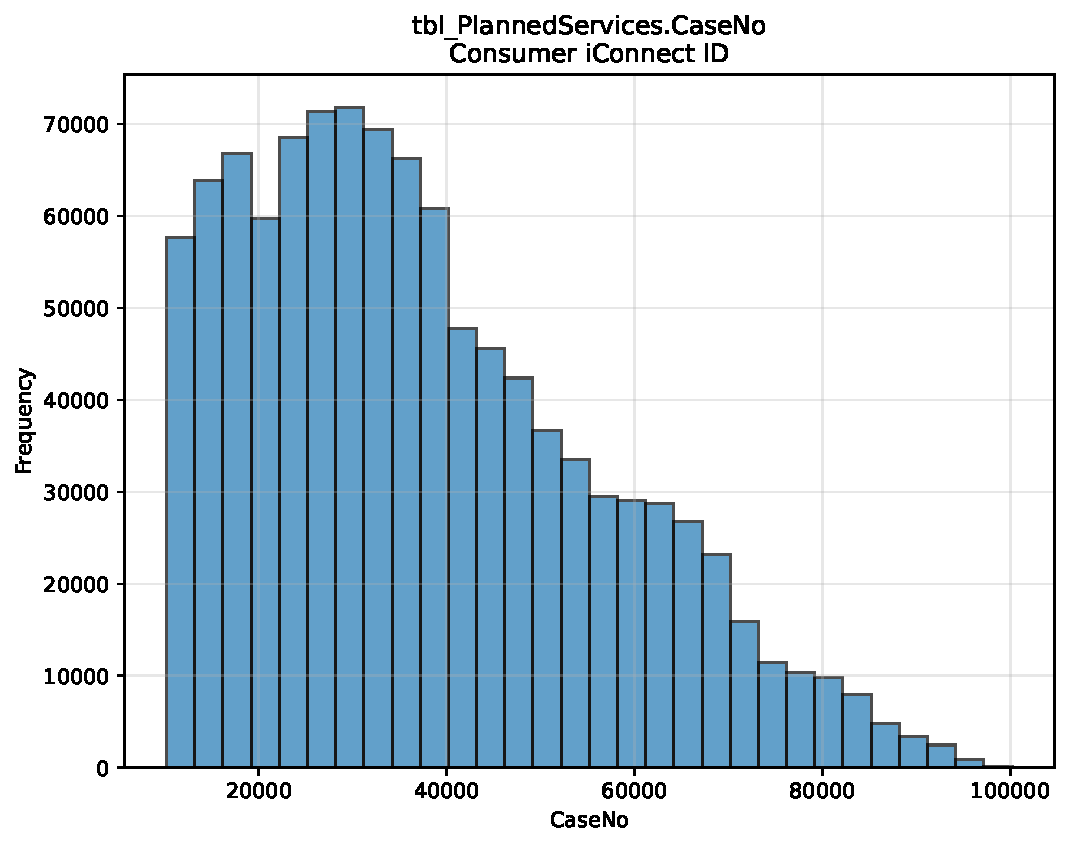
\includegraphics[width=\textwidth]{figures/dbo_tbl_PlannedServices_CaseNo.pdf}
\caption{Distribution of CaseNo in tbl\_PlannedServices}
\end{figure}\newpage

\subsection{tbl\_PlannedServices.FiscalYear}

\begin{figure}[htbp]
\centering
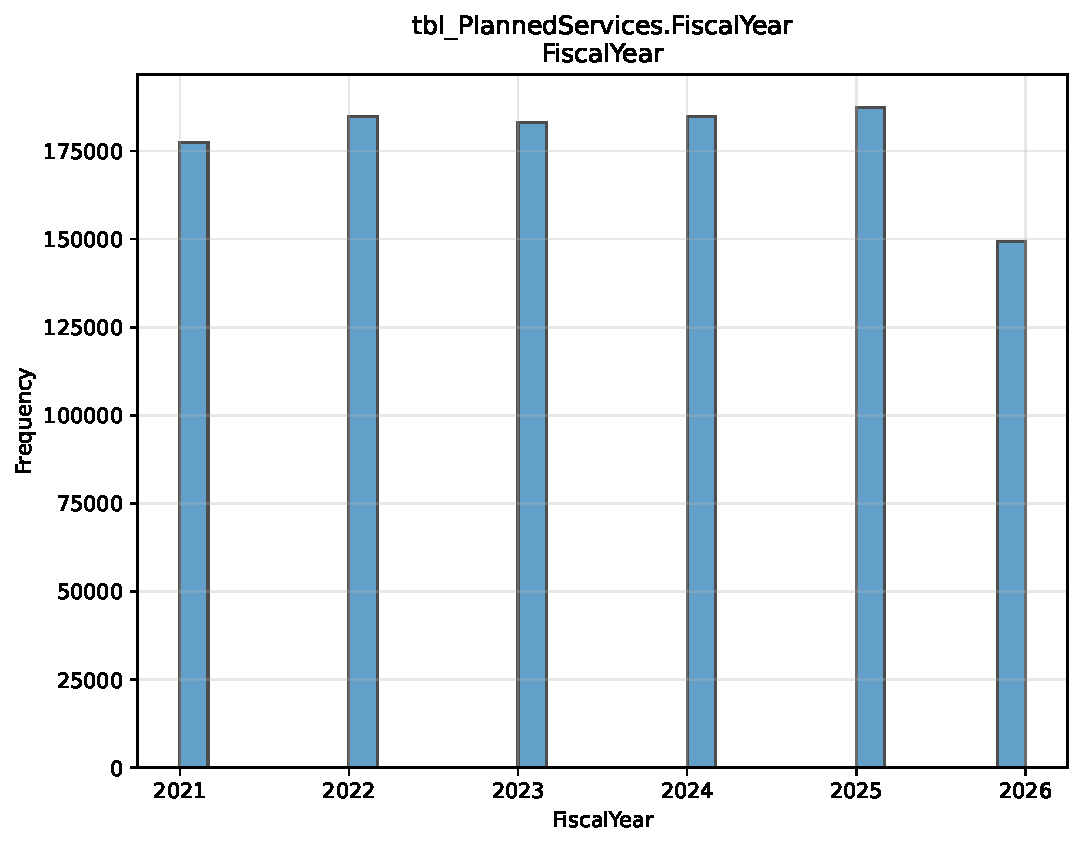
\includegraphics[width=\textwidth]{figures/dbo_tbl_PlannedServices_FiscalYear.pdf}
\caption{Distribution of FiscalYear in tbl\_PlannedServices}
\end{figure}\newpage

\subsection{tbl\_PlannedServices.UnitsPer}

\begin{figure}[htbp]
\centering
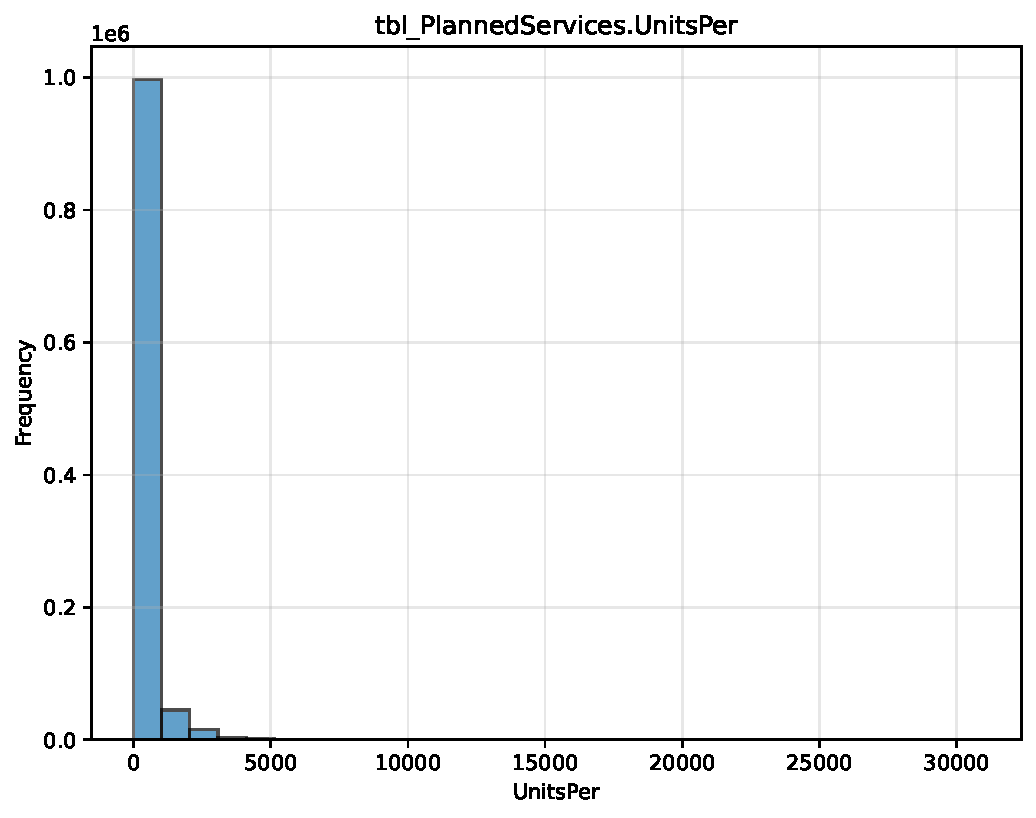
\includegraphics[width=\textwidth]{figures/dbo_tbl_PlannedServices_UnitsPer.pdf}
\caption{Distribution of UnitsPer in tbl\_PlannedServices}
\end{figure}\newpage

\subsection{tbl\_PlannedServices.TotalUnits}

\begin{figure}[htbp]
\centering
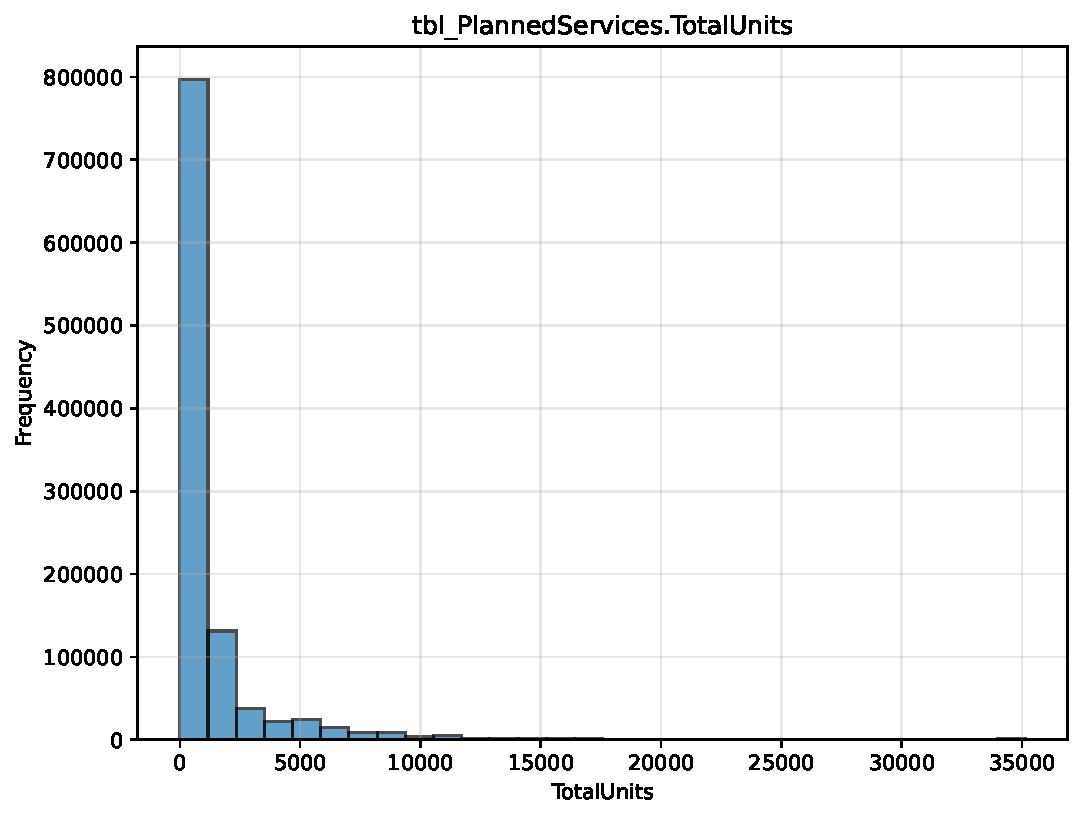
\includegraphics[width=\textwidth]{figures/dbo_tbl_PlannedServices_TotalUnits.pdf}
\caption{Distribution of TotalUnits in tbl\_PlannedServices}
\end{figure}\newpage

\subsection{tbl\_PlannedServices.AnnualizedUnits}

\begin{figure}[htbp]
\centering
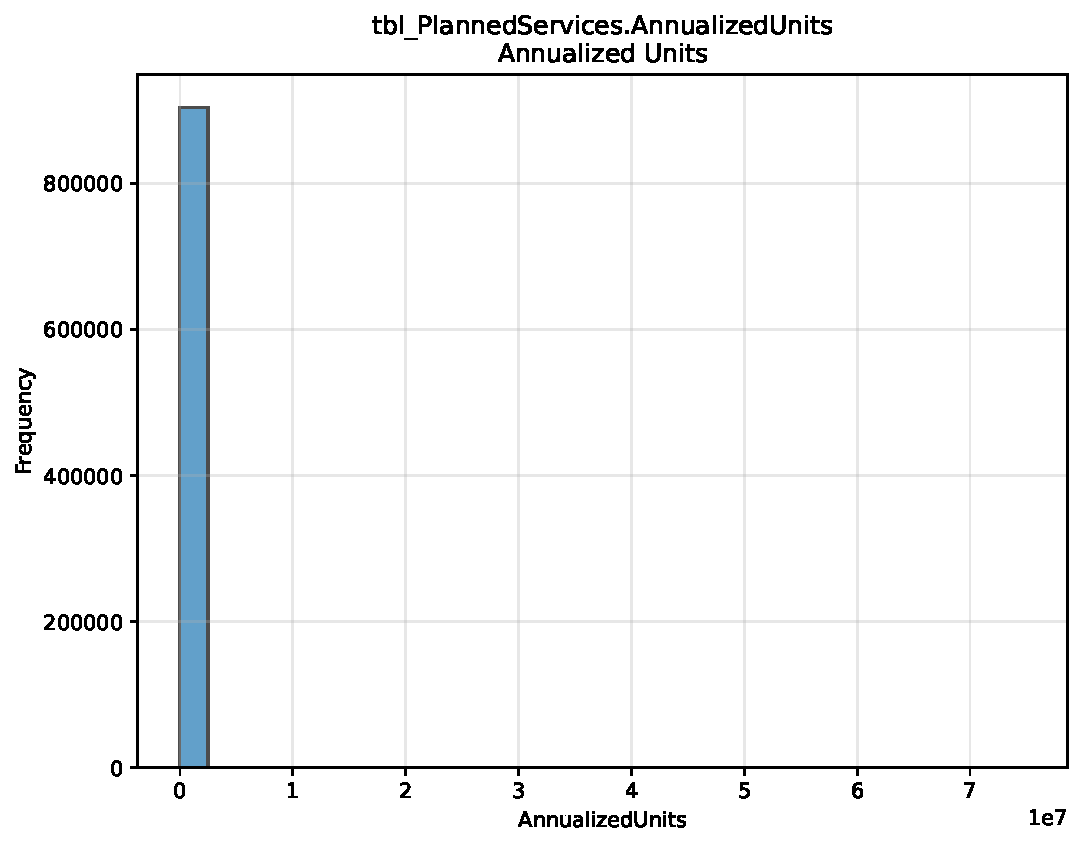
\includegraphics[width=\textwidth]{figures/dbo_tbl_PlannedServices_AnnualizedUnits.pdf}
\caption{Distribution of AnnualizedUnits in tbl\_PlannedServices}
\end{figure}\newpage

\subsection{tbl\_PlannedServices.VendorID}

\begin{figure}[htbp]
\centering
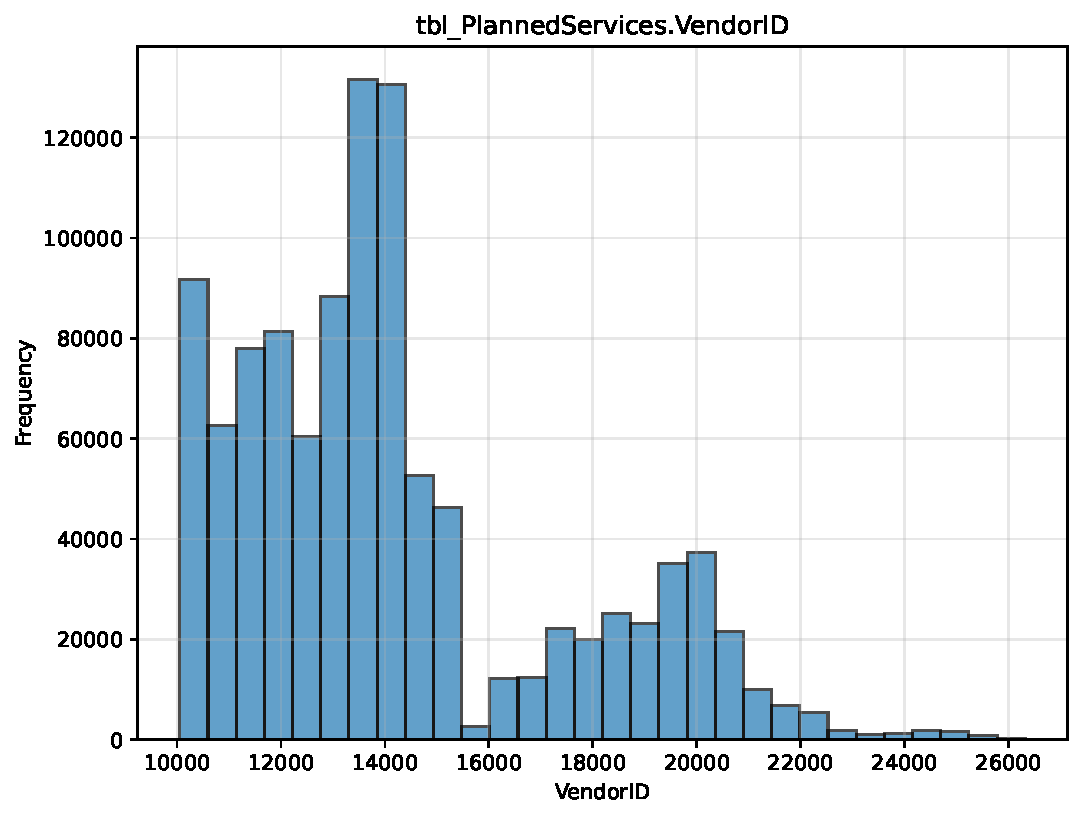
\includegraphics[width=\textwidth]{figures/dbo_tbl_PlannedServices_VendorID.pdf}
\caption{Distribution of VendorID in tbl\_PlannedServices}
\end{figure}\newpage

\subsection{tbl\_PlannedServices.Rate}

\begin{figure}[htbp]
\centering
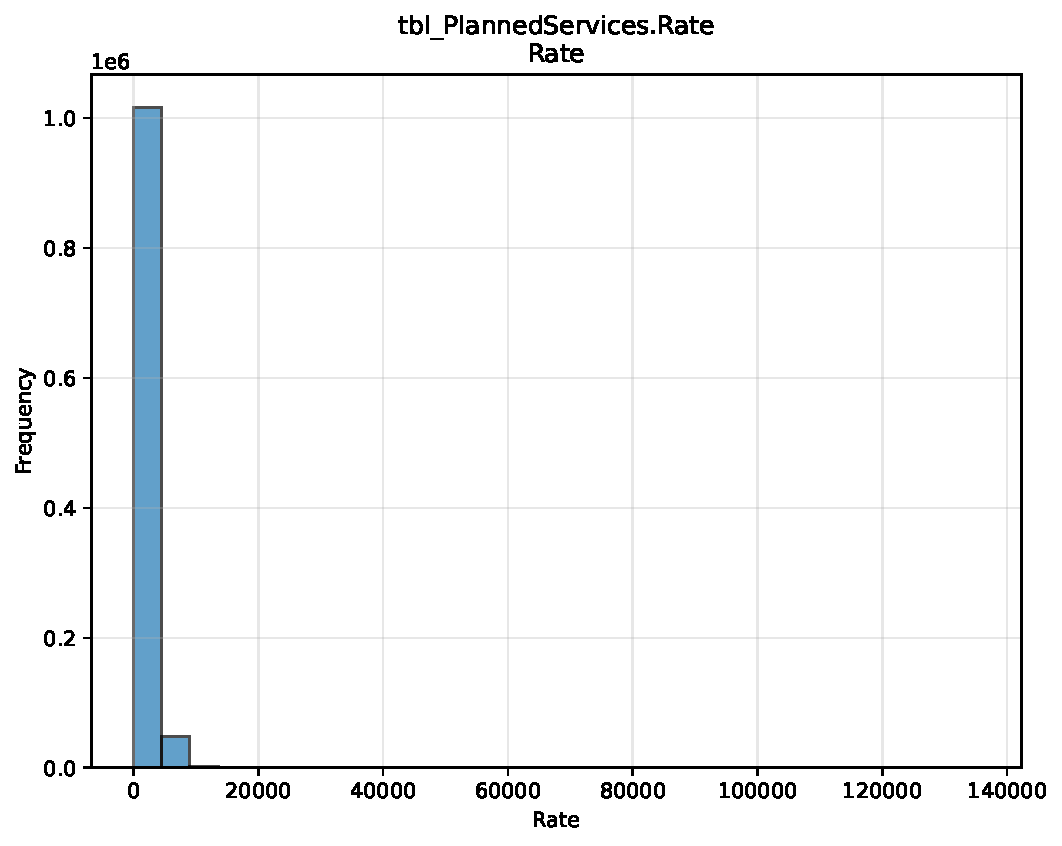
\includegraphics[width=\textwidth]{figures/dbo_tbl_PlannedServices_Rate.pdf}
\caption{Distribution of Rate in tbl\_PlannedServices}
\end{figure}\newpage

\subsection{tbl\_PlannedServices.MaxAmount}

\begin{figure}[htbp]
\centering
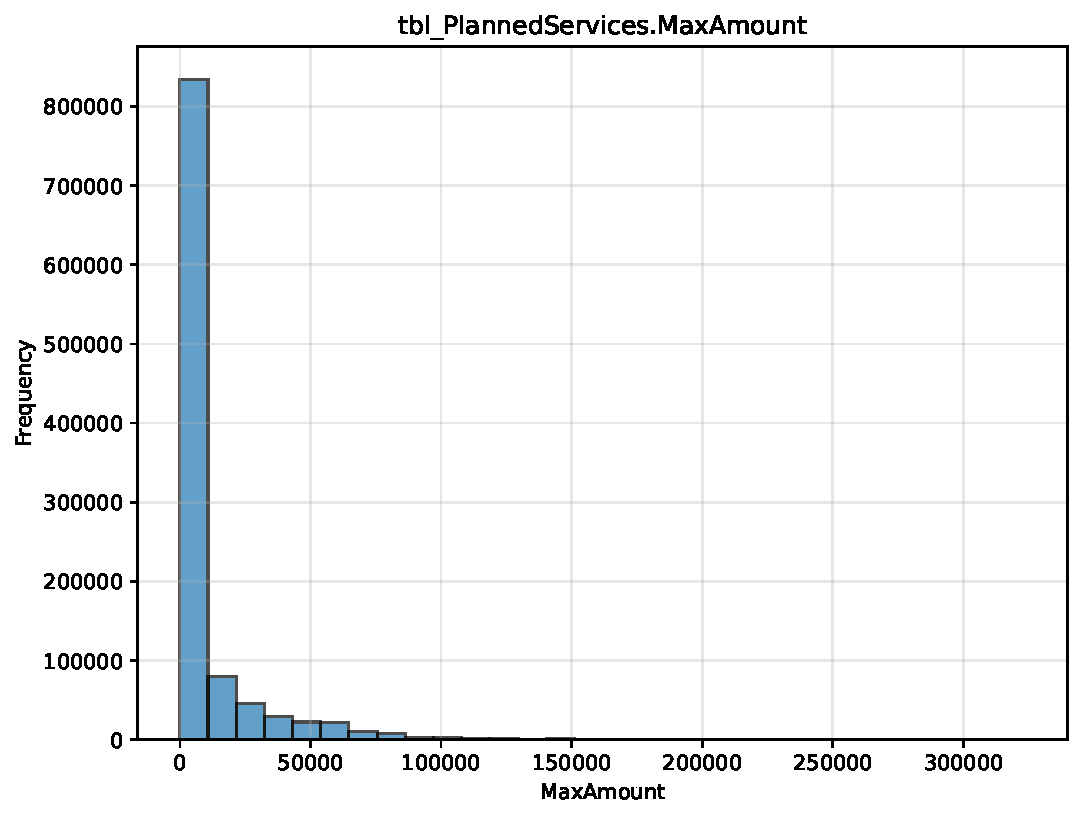
\includegraphics[width=\textwidth]{figures/dbo_tbl_PlannedServices_MaxAmount.pdf}
\caption{Distribution of MaxAmount in tbl\_PlannedServices}
\end{figure}\newpage

\subsection{tbl\_PlannedServices.AllowEVVDelivery}

\begin{figure}[htbp]
\centering
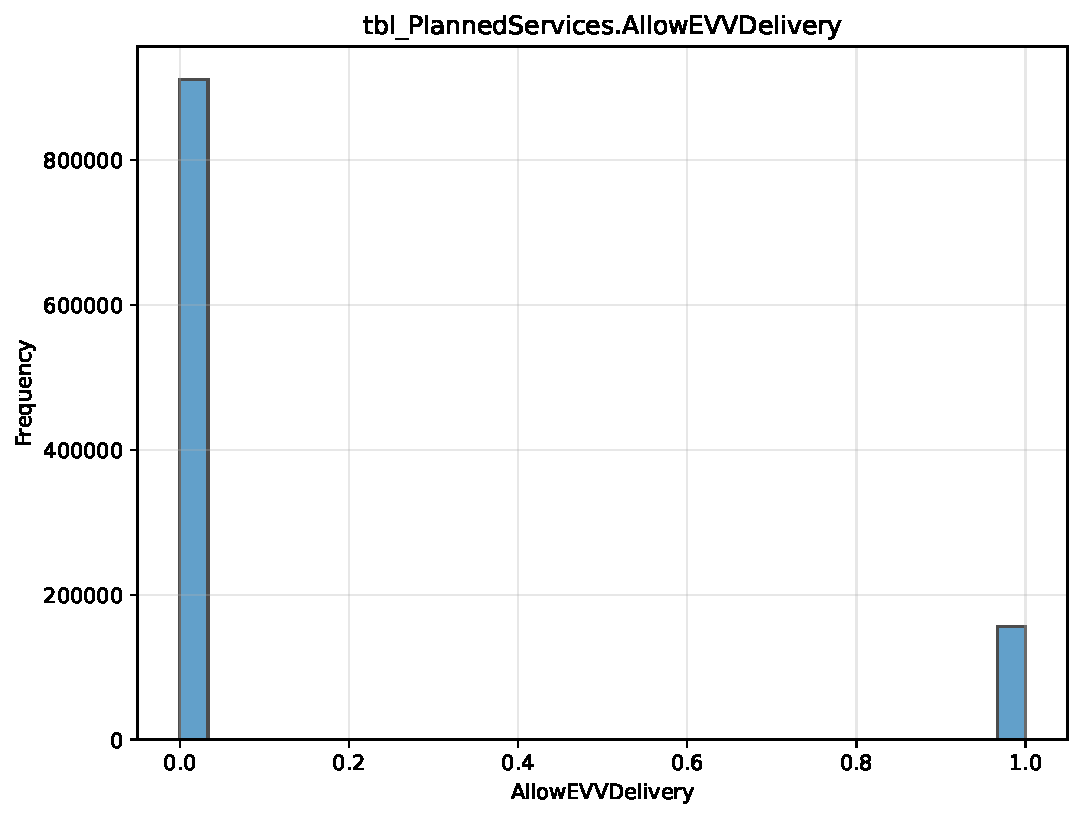
\includegraphics[width=\textwidth]{figures/dbo_tbl_PlannedServices_AllowEVVDelivery.pdf}
\caption{Distribution of AllowEVVDelivery in tbl\_PlannedServices}
\end{figure}\newpage

\subsection{tbl\_PlannedServices.PlannedServiceId}

\begin{figure}[htbp]
\centering
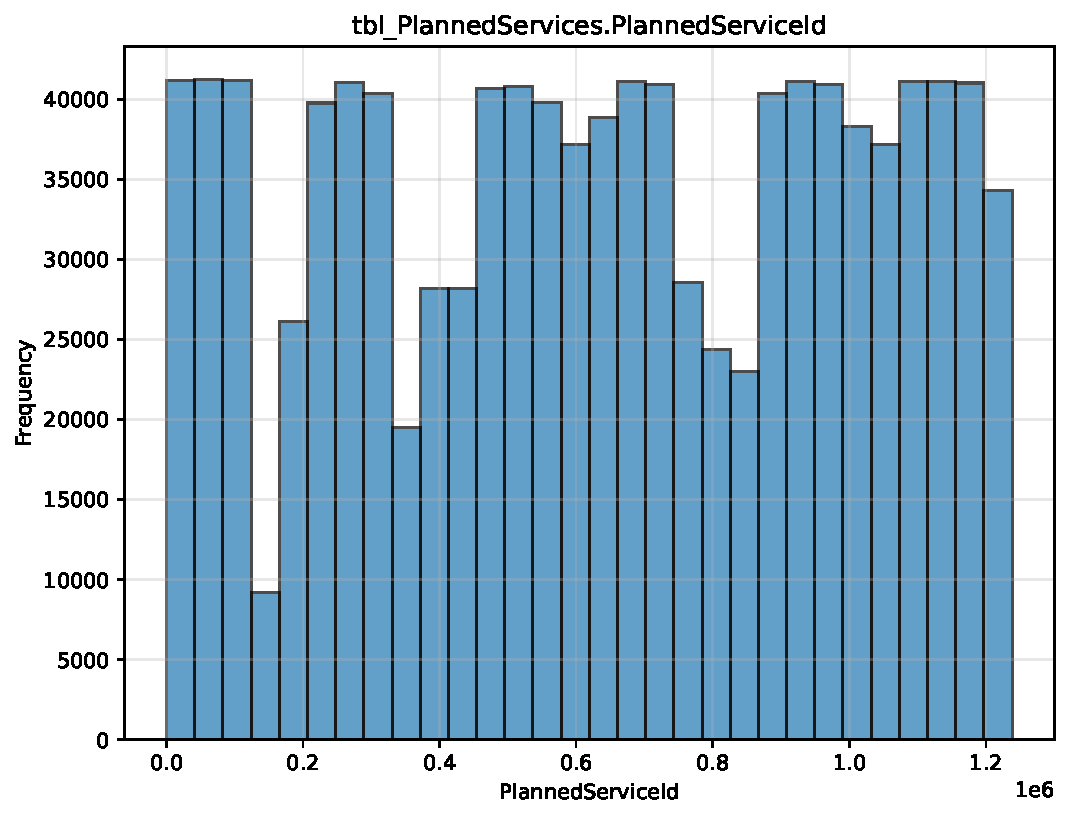
\includegraphics[width=\textwidth]{figures/dbo_tbl_PlannedServices_PlannedServiceId.pdf}
\caption{Distribution of PlannedServiceId in tbl\_PlannedServices}
\end{figure}\newpage

\subsection{tbl\_PlannedServices.PlanId}

\begin{figure}[htbp]
\centering
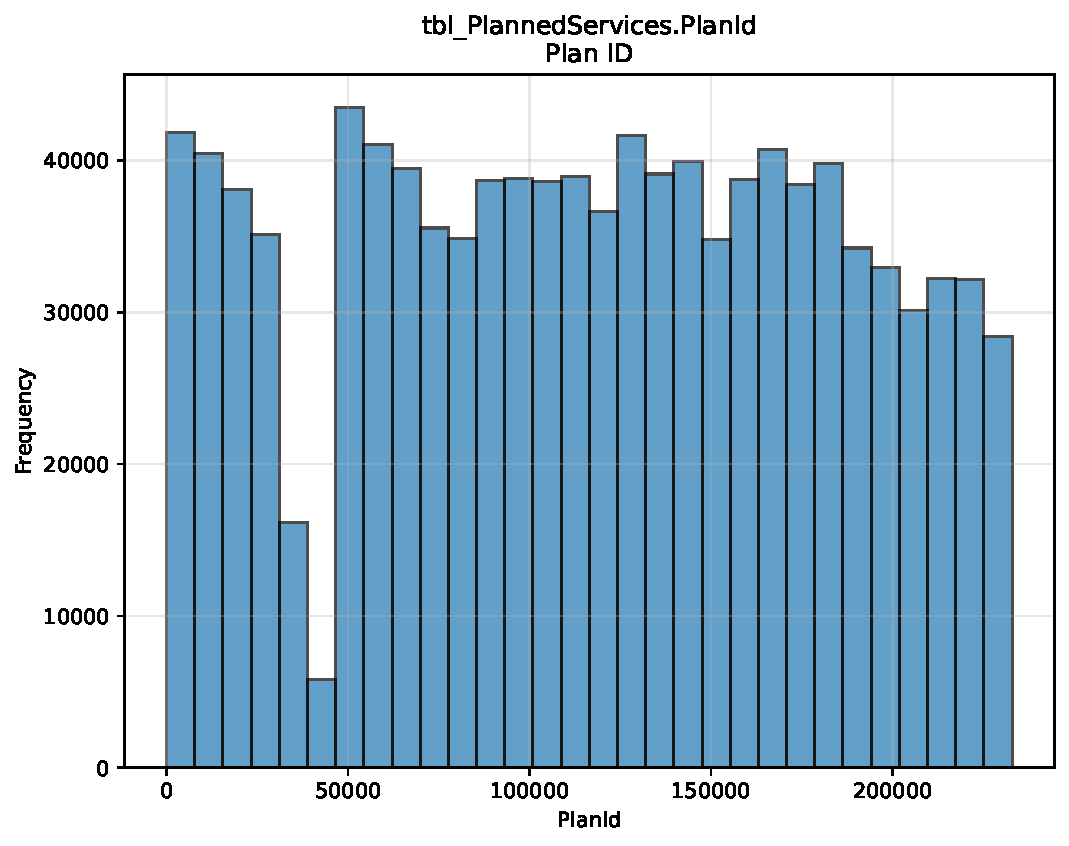
\includegraphics[width=\textwidth]{figures/dbo_tbl_PlannedServices_PlanId.pdf}
\caption{Distribution of PlanId in tbl\_PlannedServices}
\end{figure}\newpage

\subsection{tbl\_PlannedServices.ISComboCodeID}

\begin{figure}[htbp]
\centering
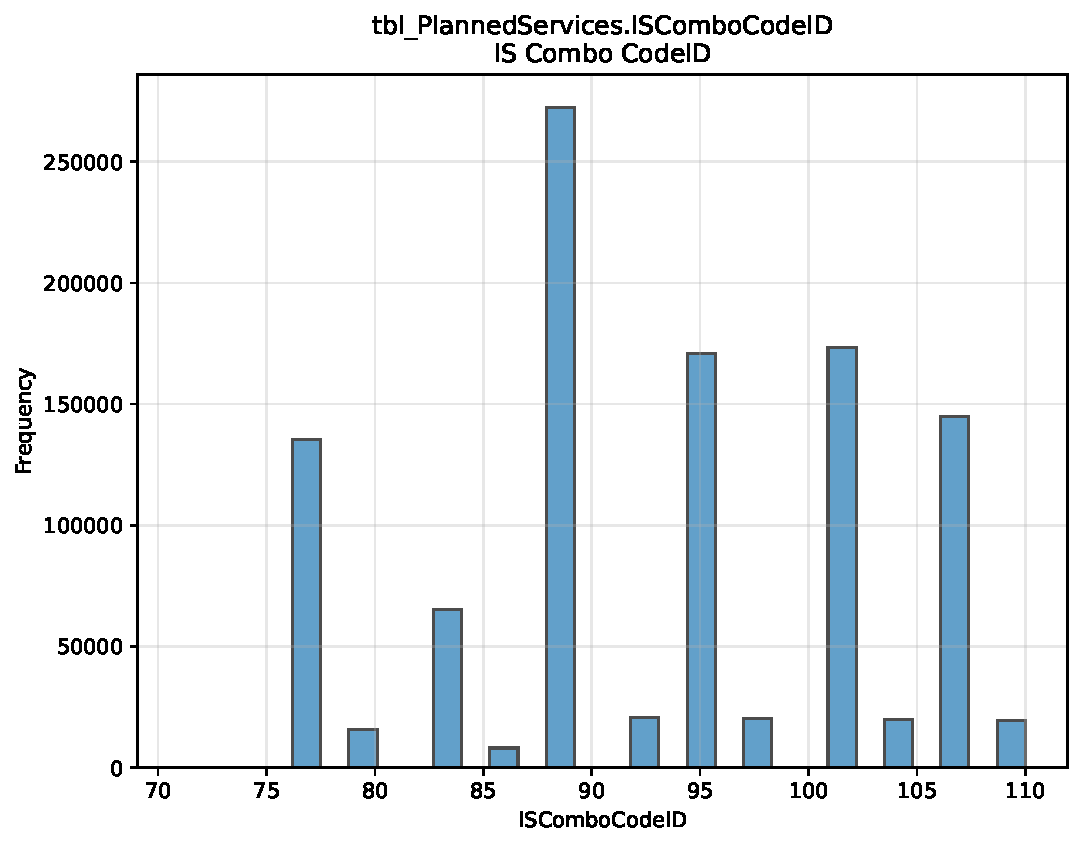
\includegraphics[width=\textwidth]{figures/dbo_tbl_PlannedServices_ISComboCodeID.pdf}
\caption{Distribution of ISComboCodeID in tbl\_PlannedServices}
\end{figure}\newpage

\subsection{tbl\_PlannedServices.VendorServicesId}

\begin{figure}[htbp]
\centering
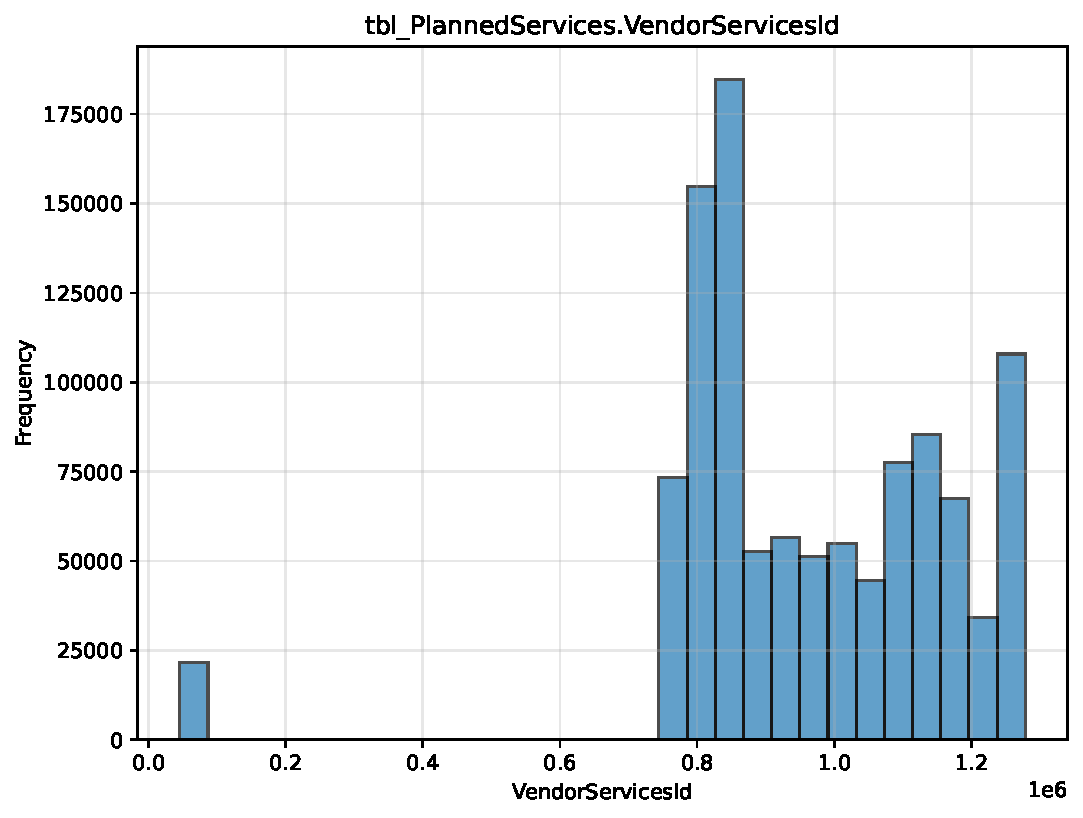
\includegraphics[width=\textwidth]{figures/dbo_tbl_PlannedServices_VendorServicesId.pdf}
\caption{Distribution of VendorServicesId in tbl\_PlannedServices}
\end{figure}\newpage

\subsection{tbl\_Plans.CaseNo}

\begin{figure}[htbp]
\centering
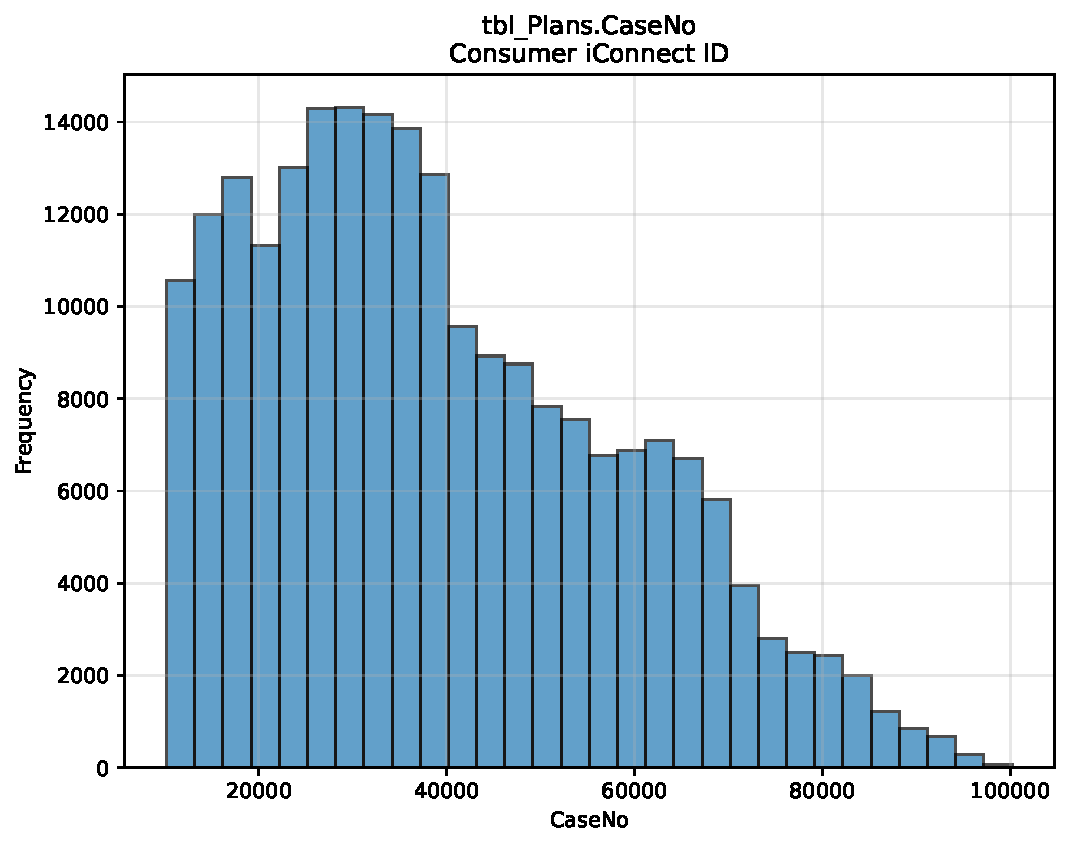
\includegraphics[width=\textwidth]{figures/dbo_tbl_Plans_CaseNo.pdf}
\caption{Distribution of CaseNo in tbl\_Plans}
\end{figure}\newpage

\subsection{tbl\_Plans.PlanId}

\begin{figure}[htbp]
\centering
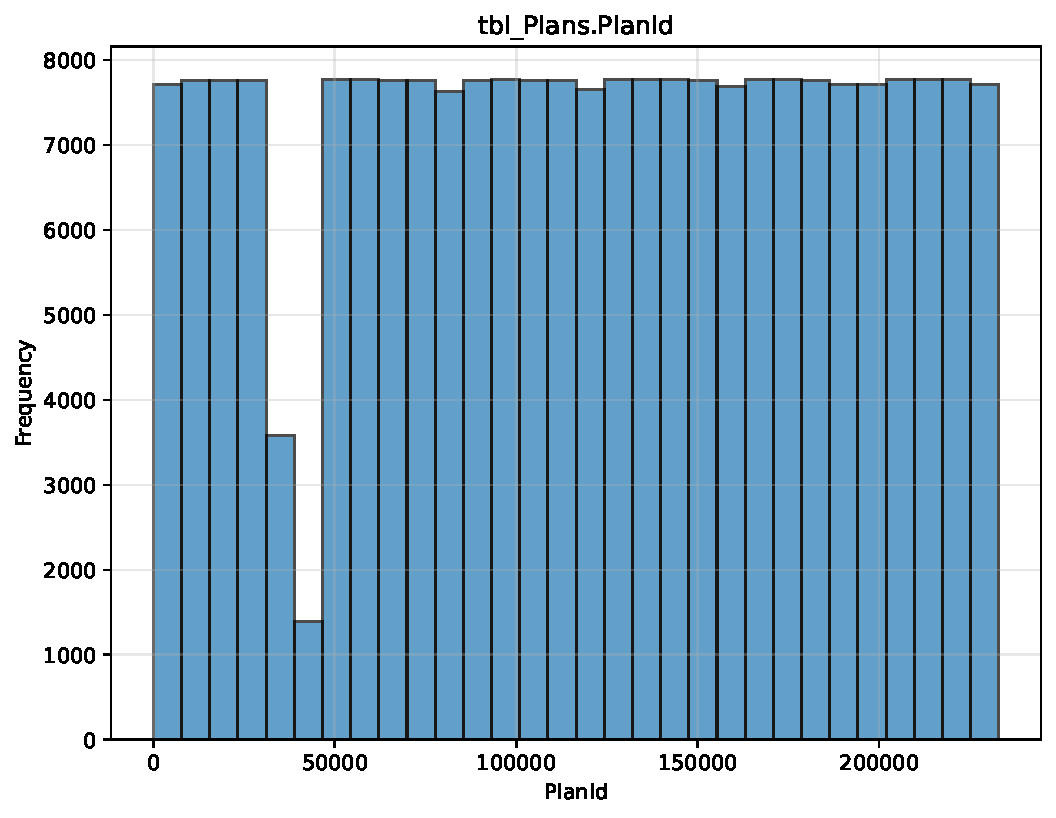
\includegraphics[width=\textwidth]{figures/dbo_tbl_Plans_PlanId.pdf}
\caption{Distribution of PlanId in tbl\_Plans}
\end{figure}\newpage

\subsection{tbl\_Plans.BudgetId}

\begin{figure}[htbp]
\centering
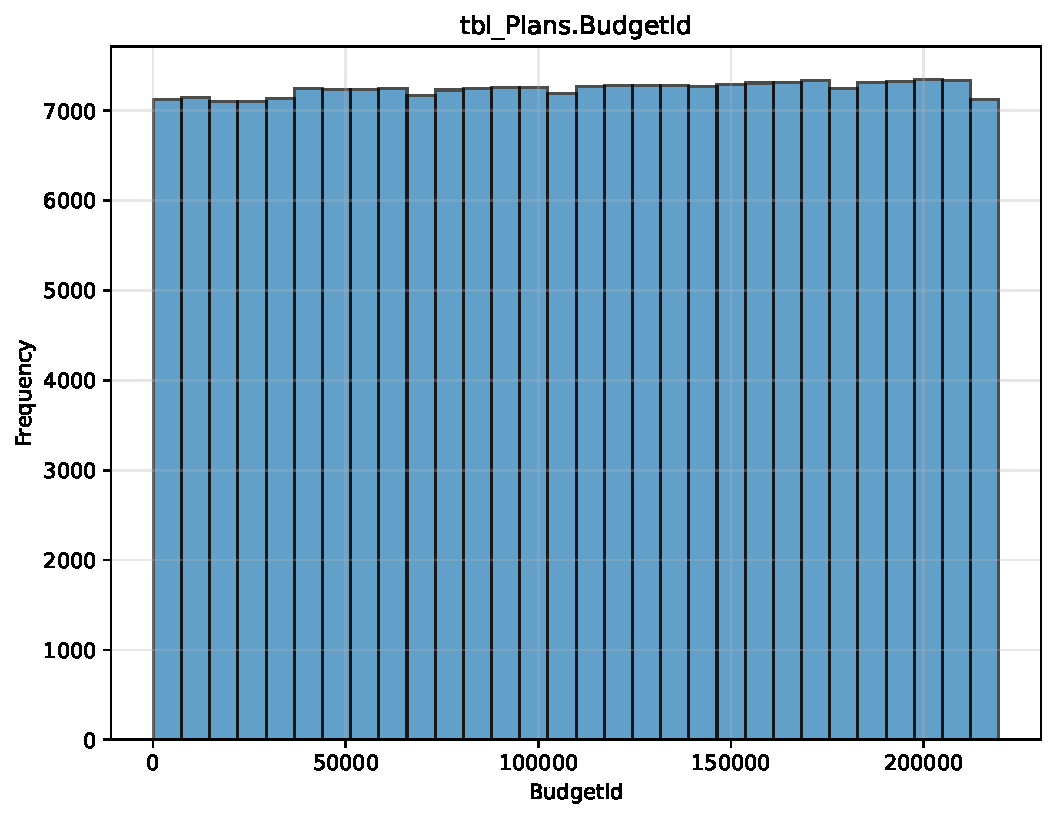
\includegraphics[width=\textwidth]{figures/dbo_tbl_Plans_BudgetId.pdf}
\caption{Distribution of BudgetId in tbl\_Plans}
\end{figure}\newpage

\subsection{tbl\_Plans.OpenId}

\begin{figure}[htbp]
\centering
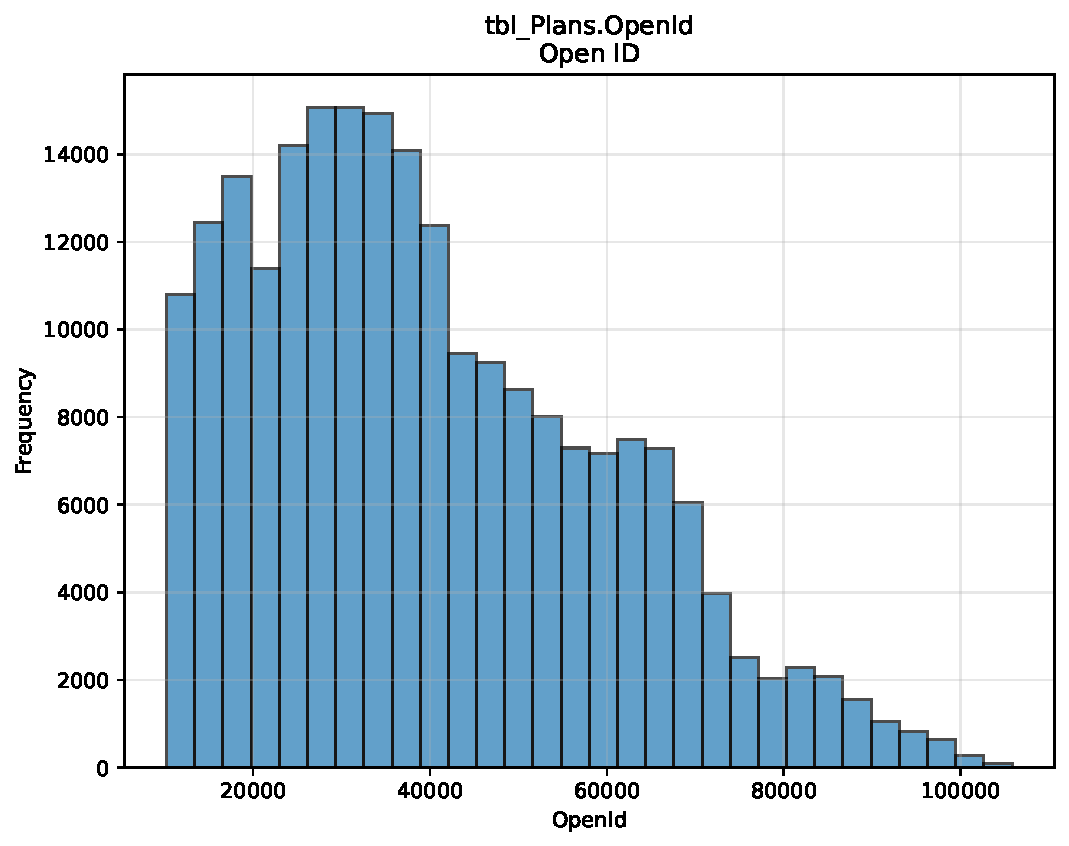
\includegraphics[width=\textwidth]{figures/dbo_tbl_Plans_OpenId.pdf}
\caption{Distribution of OpenId in tbl\_Plans}
\end{figure}\newpage

\subsection{tbl\_Plans.EnrollID}

\begin{figure}[htbp]
\centering
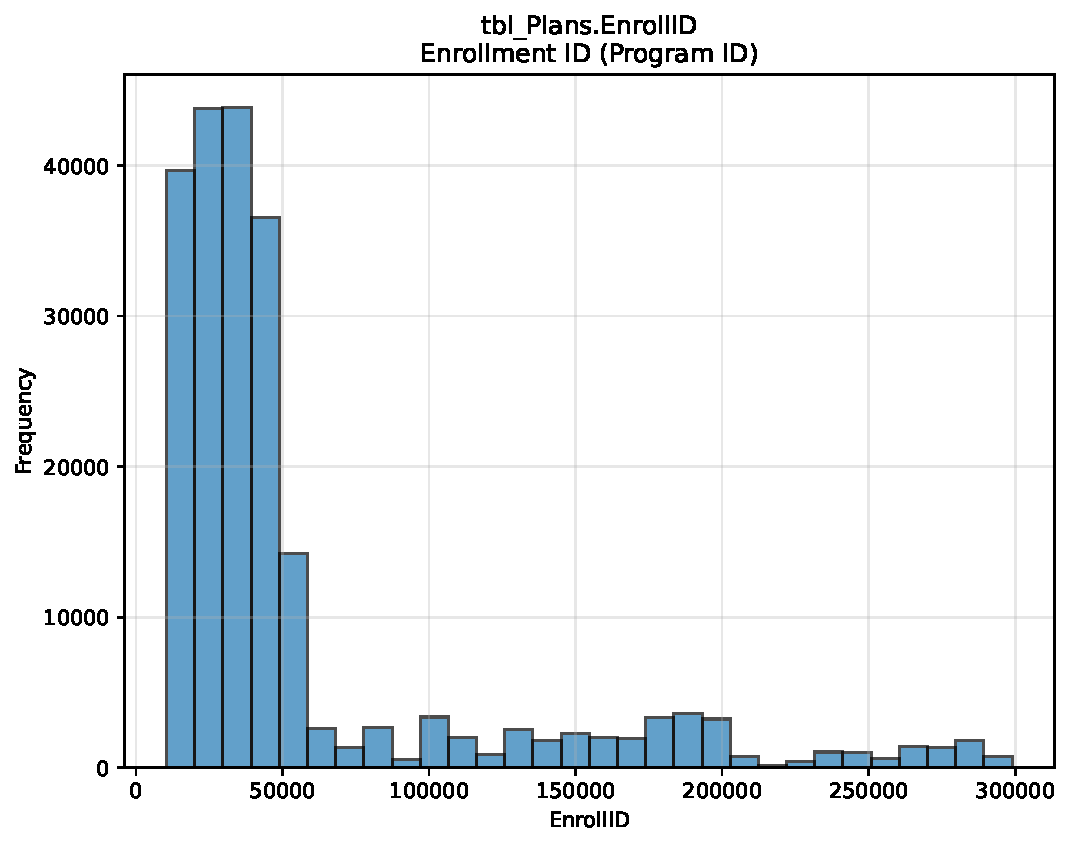
\includegraphics[width=\textwidth]{figures/dbo_tbl_Plans_EnrollID.pdf}
\caption{Distribution of EnrollID in tbl\_Plans}
\end{figure}\newpage

\subsection{tbl\_QSIAssessments.CASENO}

\begin{figure}[htbp]
\centering
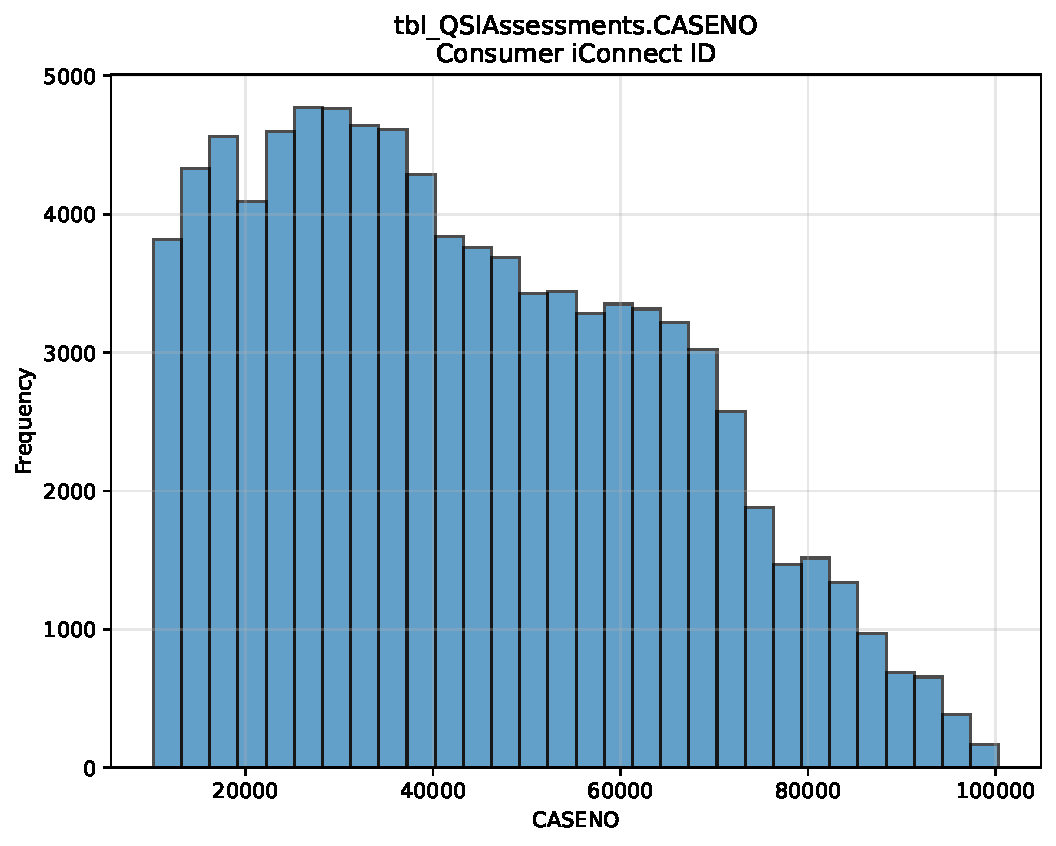
\includegraphics[width=\textwidth]{figures/dbo_tbl_QSIAssessments_CASENO.pdf}
\caption{Distribution of CASENO in tbl\_QSIAssessments}
\end{figure}\newpage

\subsection{tbl\_QSIAssessments.RaterID}

\begin{figure}[htbp]
\centering
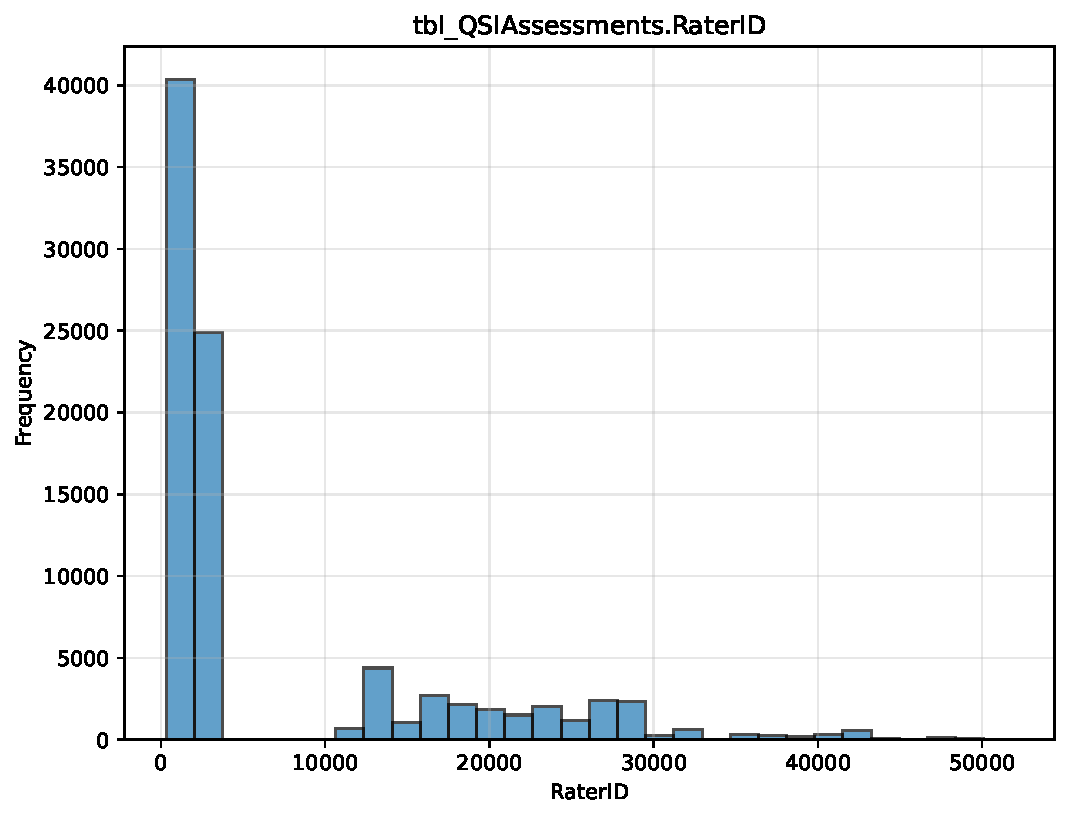
\includegraphics[width=\textwidth]{figures/dbo_tbl_QSIAssessments_RaterID.pdf}
\caption{Distribution of RaterID in tbl\_QSIAssessments}
\end{figure}\newpage

\subsection{tbl\_QSIAssessments.AssessID}

\begin{figure}[htbp]
\centering
\includegraphics[width=\textwidth]{figures/dbo_tbl_QSIAssessments_AssessID.pdf}
\caption{Distribution of AssessID in tbl\_QSIAssessments}
\end{figure}\newpage

\subsection{tbl\_QSIAssessments.LegacyAssessID}

\begin{figure}[htbp]
\centering
\includegraphics[width=\textwidth]{figures/dbo_tbl_QSIAssessments_LegacyAssessID.pdf}
\caption{Distribution of LegacyAssessID in tbl\_QSIAssessments}
\end{figure}\newpage

\subsection{tbl\_QSIAssessmentsLegacy.RATERID}

\begin{figure}[htbp]
\centering
\includegraphics[width=\textwidth]{figures/dbo_tbl_QSIAssessmentsLegacy_RATERID.pdf}
\caption{Distribution of RATERID in tbl\_QSIAssessmentsLegacy}
\end{figure}\newpage

\subsection{tbl\_QSIAssessmentsLegacy.Q14}

\begin{figure}[htbp]
\centering
\includegraphics[width=\textwidth]{figures/dbo_tbl_QSIAssessmentsLegacy_Q14.pdf}
\caption{Distribution of Q14 in tbl\_QSIAssessmentsLegacy}
\end{figure}\newpage

\subsection{tbl\_QSIAssessmentsLegacy.Q15}

\begin{figure}[htbp]
\centering
\includegraphics[width=\textwidth]{figures/dbo_tbl_QSIAssessmentsLegacy_Q15.pdf}
\caption{Distribution of Q15 in tbl\_QSIAssessmentsLegacy}
\end{figure}\newpage

\subsection{tbl\_QSIAssessmentsLegacy.Q16}

\begin{figure}[htbp]
\centering
\includegraphics[width=\textwidth]{figures/dbo_tbl_QSIAssessmentsLegacy_Q16.pdf}
\caption{Distribution of Q16 in tbl\_QSIAssessmentsLegacy}
\end{figure}\newpage

\subsection{tbl\_QSIAssessmentsLegacy.Q17}

\begin{figure}[htbp]
\centering
\includegraphics[width=\textwidth]{figures/dbo_tbl_QSIAssessmentsLegacy_Q17.pdf}
\caption{Distribution of Q17 in tbl\_QSIAssessmentsLegacy}
\end{figure}\newpage

\subsection{tbl\_QSIAssessmentsLegacy.Q18}

\begin{figure}[htbp]
\centering
\includegraphics[width=\textwidth]{figures/dbo_tbl_QSIAssessmentsLegacy_Q18.pdf}
\caption{Distribution of Q18 in tbl\_QSIAssessmentsLegacy}
\end{figure}\newpage

\subsection{tbl\_QSIAssessmentsLegacy.Q19}

\begin{figure}[htbp]
\centering
\includegraphics[width=\textwidth]{figures/dbo_tbl_QSIAssessmentsLegacy_Q19.pdf}
\caption{Distribution of Q19 in tbl\_QSIAssessmentsLegacy}
\end{figure}\newpage

\subsection{tbl\_QSIAssessmentsLegacy.Q20}

\begin{figure}[htbp]
\centering
\includegraphics[width=\textwidth]{figures/dbo_tbl_QSIAssessmentsLegacy_Q20.pdf}
\caption{Distribution of Q20 in tbl\_QSIAssessmentsLegacy}
\end{figure}\newpage

\subsection{tbl\_QSIAssessmentsLegacy.Q21}

\begin{figure}[htbp]
\centering
\includegraphics[width=\textwidth]{figures/dbo_tbl_QSIAssessmentsLegacy_Q21.pdf}
\caption{Distribution of Q21 in tbl\_QSIAssessmentsLegacy}
\end{figure}\newpage

\subsection{tbl\_QSIAssessmentsLegacy.Q22}

\begin{figure}[htbp]
\centering
\includegraphics[width=\textwidth]{figures/dbo_tbl_QSIAssessmentsLegacy_Q22.pdf}
\caption{Distribution of Q22 in tbl\_QSIAssessmentsLegacy}
\end{figure}\newpage

\subsection{tbl\_QSIAssessmentsLegacy.Q23}

\begin{figure}[htbp]
\centering
\includegraphics[width=\textwidth]{figures/dbo_tbl_QSIAssessmentsLegacy_Q23.pdf}
\caption{Distribution of Q23 in tbl\_QSIAssessmentsLegacy}
\end{figure}\newpage

\subsection{tbl\_QSIAssessmentsLegacy.Q24}

\begin{figure}[htbp]
\centering
\includegraphics[width=\textwidth]{figures/dbo_tbl_QSIAssessmentsLegacy_Q24.pdf}
\caption{Distribution of Q24 in tbl\_QSIAssessmentsLegacy}
\end{figure}\newpage

\subsection{tbl\_QSIAssessmentsLegacy.Q25}

\begin{figure}[htbp]
\centering
\includegraphics[width=\textwidth]{figures/dbo_tbl_QSIAssessmentsLegacy_Q25.pdf}
\caption{Distribution of Q25 in tbl\_QSIAssessmentsLegacy}
\end{figure}\newpage

\subsection{tbl\_QSIAssessmentsLegacy.Q26}

\begin{figure}[htbp]
\centering
\includegraphics[width=\textwidth]{figures/dbo_tbl_QSIAssessmentsLegacy_Q26.pdf}
\caption{Distribution of Q26 in tbl\_QSIAssessmentsLegacy}
\end{figure}\newpage

\subsection{tbl\_QSIAssessmentsLegacy.Q27}

\begin{figure}[htbp]
\centering
\includegraphics[width=\textwidth]{figures/dbo_tbl_QSIAssessmentsLegacy_Q27.pdf}
\caption{Distribution of Q27 in tbl\_QSIAssessmentsLegacy}
\end{figure}\newpage

\subsection{tbl\_QSIAssessmentsLegacy.Q28}

\begin{figure}[htbp]
\centering
\includegraphics[width=\textwidth]{figures/dbo_tbl_QSIAssessmentsLegacy_Q28.pdf}
\caption{Distribution of Q28 in tbl\_QSIAssessmentsLegacy}
\end{figure}\newpage

\subsection{tbl\_QSIAssessmentsLegacy.Q29}

\begin{figure}[htbp]
\centering
\includegraphics[width=\textwidth]{figures/dbo_tbl_QSIAssessmentsLegacy_Q29.pdf}
\caption{Distribution of Q29 in tbl\_QSIAssessmentsLegacy}
\end{figure}\newpage

\subsection{tbl\_QSIAssessmentsLegacy.Q30}

\begin{figure}[htbp]
\centering
\includegraphics[width=\textwidth]{figures/dbo_tbl_QSIAssessmentsLegacy_Q30.pdf}
\caption{Distribution of Q30 in tbl\_QSIAssessmentsLegacy}
\end{figure}\newpage

\subsection{tbl\_QSIAssessmentsLegacy.Q30a}

\begin{figure}[htbp]
\centering
\includegraphics[width=\textwidth]{figures/dbo_tbl_QSIAssessmentsLegacy_Q30a.pdf}
\caption{Distribution of Q30a in tbl\_QSIAssessmentsLegacy}
\end{figure}\newpage

\subsection{tbl\_QSIAssessmentsLegacy.Q30b}

\begin{figure}[htbp]
\centering
\includegraphics[width=\textwidth]{figures/dbo_tbl_QSIAssessmentsLegacy_Q30b.pdf}
\caption{Distribution of Q30b in tbl\_QSIAssessmentsLegacy}
\end{figure}\newpage

\subsection{tbl\_QSIAssessmentsLegacy.Q31}

\begin{figure}[htbp]
\centering
\includegraphics[width=\textwidth]{figures/dbo_tbl_QSIAssessmentsLegacy_Q31.pdf}
\caption{Distribution of Q31 in tbl\_QSIAssessmentsLegacy}
\end{figure}\newpage

\subsection{tbl\_QSIAssessmentsLegacy.Q32}

\begin{figure}[htbp]
\centering
\includegraphics[width=\textwidth]{figures/dbo_tbl_QSIAssessmentsLegacy_Q32.pdf}
\caption{Distribution of Q32 in tbl\_QSIAssessmentsLegacy}
\end{figure}\newpage

\subsection{tbl\_QSIAssessmentsLegacy.Q33}

\begin{figure}[htbp]
\centering
\includegraphics[width=\textwidth]{figures/dbo_tbl_QSIAssessmentsLegacy_Q33.pdf}
\caption{Distribution of Q33 in tbl\_QSIAssessmentsLegacy}
\end{figure}\newpage

\subsection{tbl\_QSIAssessmentsLegacy.Q34}

\begin{figure}[htbp]
\centering
\includegraphics[width=\textwidth]{figures/dbo_tbl_QSIAssessmentsLegacy_Q34.pdf}
\caption{Distribution of Q34 in tbl\_QSIAssessmentsLegacy}
\end{figure}\newpage

\subsection{tbl\_QSIAssessmentsLegacy.Q35}

\begin{figure}[htbp]
\centering
\includegraphics[width=\textwidth]{figures/dbo_tbl_QSIAssessmentsLegacy_Q35.pdf}
\caption{Distribution of Q35 in tbl\_QSIAssessmentsLegacy}
\end{figure}\newpage

\subsection{tbl\_QSIAssessmentsLegacy.Q36}

\begin{figure}[htbp]
\centering
\includegraphics[width=\textwidth]{figures/dbo_tbl_QSIAssessmentsLegacy_Q36.pdf}
\caption{Distribution of Q36 in tbl\_QSIAssessmentsLegacy}
\end{figure}\newpage

\subsection{tbl\_QSIAssessmentsLegacy.Q37}

\begin{figure}[htbp]
\centering
\includegraphics[width=\textwidth]{figures/dbo_tbl_QSIAssessmentsLegacy_Q37.pdf}
\caption{Distribution of Q37 in tbl\_QSIAssessmentsLegacy}
\end{figure}\newpage

\subsection{tbl\_QSIAssessmentsLegacy.Q38}

\begin{figure}[htbp]
\centering
\includegraphics[width=\textwidth]{figures/dbo_tbl_QSIAssessmentsLegacy_Q38.pdf}
\caption{Distribution of Q38 in tbl\_QSIAssessmentsLegacy}
\end{figure}\newpage

\subsection{tbl\_QSIAssessmentsLegacy.Q39}

\begin{figure}[htbp]
\centering
\includegraphics[width=\textwidth]{figures/dbo_tbl_QSIAssessmentsLegacy_Q39.pdf}
\caption{Distribution of Q39 in tbl\_QSIAssessmentsLegacy}
\end{figure}\newpage

\subsection{tbl\_QSIAssessmentsLegacy.Q40}

\begin{figure}[htbp]
\centering
\includegraphics[width=\textwidth]{figures/dbo_tbl_QSIAssessmentsLegacy_Q40.pdf}
\caption{Distribution of Q40 in tbl\_QSIAssessmentsLegacy}
\end{figure}\newpage

\subsection{tbl\_QSIAssessmentsLegacy.Q41}

\begin{figure}[htbp]
\centering
\includegraphics[width=\textwidth]{figures/dbo_tbl_QSIAssessmentsLegacy_Q41.pdf}
\caption{Distribution of Q41 in tbl\_QSIAssessmentsLegacy}
\end{figure}\newpage

\subsection{tbl\_QSIAssessmentsLegacy.Q42}

\begin{figure}[htbp]
\centering
\includegraphics[width=\textwidth]{figures/dbo_tbl_QSIAssessmentsLegacy_Q42.pdf}
\caption{Distribution of Q42 in tbl\_QSIAssessmentsLegacy}
\end{figure}\newpage

\subsection{tbl\_QSIAssessmentsLegacy.Q43}

\begin{figure}[htbp]
\centering
\includegraphics[width=\textwidth]{figures/dbo_tbl_QSIAssessmentsLegacy_Q43.pdf}
\caption{Distribution of Q43 in tbl\_QSIAssessmentsLegacy}
\end{figure}\newpage

\subsection{tbl\_QSIAssessmentsLegacy.Q44}

\begin{figure}[htbp]
\centering
\includegraphics[width=\textwidth]{figures/dbo_tbl_QSIAssessmentsLegacy_Q44.pdf}
\caption{Distribution of Q44 in tbl\_QSIAssessmentsLegacy}
\end{figure}\newpage

\subsection{tbl\_QSIAssessmentsLegacy.Q45}

\begin{figure}[htbp]
\centering
\includegraphics[width=\textwidth]{figures/dbo_tbl_QSIAssessmentsLegacy_Q45.pdf}
\caption{Distribution of Q45 in tbl\_QSIAssessmentsLegacy}
\end{figure}\newpage

\subsection{tbl\_QSIAssessmentsLegacy.Q46}

\begin{figure}[htbp]
\centering
\includegraphics[width=\textwidth]{figures/dbo_tbl_QSIAssessmentsLegacy_Q46.pdf}
\caption{Distribution of Q46 in tbl\_QSIAssessmentsLegacy}
\end{figure}\newpage

\subsection{tbl\_QSIAssessmentsLegacy.Q47}

\begin{figure}[htbp]
\centering
\includegraphics[width=\textwidth]{figures/dbo_tbl_QSIAssessmentsLegacy_Q47.pdf}
\caption{Distribution of Q47 in tbl\_QSIAssessmentsLegacy}
\end{figure}\newpage

\subsection{tbl\_QSIAssessmentsLegacy.Q48}

\begin{figure}[htbp]
\centering
\includegraphics[width=\textwidth]{figures/dbo_tbl_QSIAssessmentsLegacy_Q48.pdf}
\caption{Distribution of Q48 in tbl\_QSIAssessmentsLegacy}
\end{figure}\newpage

\subsection{tbl\_QSIAssessmentsLegacy.Q49}

\begin{figure}[htbp]
\centering
\includegraphics[width=\textwidth]{figures/dbo_tbl_QSIAssessmentsLegacy_Q49.pdf}
\caption{Distribution of Q49 in tbl\_QSIAssessmentsLegacy}
\end{figure}\newpage

\subsection{tbl\_QSIAssessmentsLegacy.Q49a}

\begin{figure}[htbp]
\centering
\includegraphics[width=\textwidth]{figures/dbo_tbl_QSIAssessmentsLegacy_Q49a.pdf}
\caption{Distribution of Q49a in tbl\_QSIAssessmentsLegacy}
\end{figure}\newpage

\subsection{tbl\_QSIAssessmentsLegacy.FLEVEL}

\begin{figure}[htbp]
\centering
\includegraphics[width=\textwidth]{figures/dbo_tbl_QSIAssessmentsLegacy_FLEVEL.pdf}
\caption{Distribution of FLEVEL in tbl\_QSIAssessmentsLegacy}
\end{figure}\newpage

\subsection{tbl\_QSIAssessmentsLegacy.BLEVEL}

\begin{figure}[htbp]
\centering
\includegraphics[width=\textwidth]{figures/dbo_tbl_QSIAssessmentsLegacy_BLEVEL.pdf}
\caption{Distribution of BLEVEL in tbl\_QSIAssessmentsLegacy}
\end{figure}\newpage

\subsection{tbl\_QSIAssessmentsLegacy.PLEVEL}

\begin{figure}[htbp]
\centering
\includegraphics[width=\textwidth]{figures/dbo_tbl_QSIAssessmentsLegacy_PLEVEL.pdf}
\caption{Distribution of PLEVEL in tbl\_QSIAssessmentsLegacy}
\end{figure}\newpage

\subsection{tbl\_QSIAssessmentsLegacy.LOSRI}

\begin{figure}[htbp]
\centering
\includegraphics[width=\textwidth]{figures/dbo_tbl_QSIAssessmentsLegacy_LOSRI.pdf}
\caption{Distribution of LOSRI in tbl\_QSIAssessmentsLegacy}
\end{figure}\newpage

\subsection{tbl\_QSIAssessmentsLegacy.ASSESSID}

\begin{figure}[htbp]
\centering
\includegraphics[width=\textwidth]{figures/dbo_tbl_QSIAssessmentsLegacy_ASSESSID.pdf}
\caption{Distribution of ASSESSID in tbl\_QSIAssessmentsLegacy}
\end{figure}\newpage

\subsection{tbl\_QSIQuestions.QuestionAssoc}

\begin{figure}[htbp]
\centering
\includegraphics[width=\textwidth]{figures/dbo_tbl_QSIQuestions_QuestionAssoc.pdf}
\caption{Distribution of QuestionAssoc in tbl\_QSIQuestions}
\end{figure}\newpage

\subsection{tbl\_Rates.UnitCost}

\begin{figure}[htbp]
\centering
\includegraphics[width=\textwidth]{figures/dbo_tbl_Rates_UnitCost.pdf}
\caption{Distribution of UnitCost in tbl\_Rates}
\end{figure}\newpage

\subsection{tbl\_Rates.UserStamp}

\begin{figure}[htbp]
\centering
\includegraphics[width=\textwidth]{figures/dbo_tbl_Rates_UserStamp.pdf}
\caption{Distribution of UserStamp in tbl\_Rates}
\end{figure}\newpage

\subsection{tbl\_Rates.ServiceCodeUnitCostID}

\begin{figure}[htbp]
\centering
\includegraphics[width=\textwidth]{figures/dbo_tbl_Rates_ServiceCodeUnitCostID.pdf}
\caption{Distribution of ServiceCodeUnitCostID in tbl\_Rates}
\end{figure}\newpage

\subsection{tbl\_Rates.ServiceCodesId}

\begin{figure}[htbp]
\centering
\includegraphics[width=\textwidth]{figures/dbo_tbl_Rates_ServiceCodesId.pdf}
\caption{Distribution of ServiceCodesId in tbl\_Rates}
\end{figure}\newpage

\subsection{tbl\_SANs.CaseNo}

\begin{figure}[htbp]
\centering
\includegraphics[width=\textwidth]{figures/dbo_tbl_SANs_CaseNo.pdf}
\caption{Distribution of CaseNo in tbl\_SANs}
\end{figure}\newpage

\subsection{tbl\_SANs.SanID}

\begin{figure}[htbp]
\centering
\includegraphics[width=\textwidth]{figures/dbo_tbl_SANs_SanID.pdf}
\caption{Distribution of SanID in tbl\_SANs}
\end{figure}\newpage

\subsection{tbl\_SANs.PlanID}

\begin{figure}[htbp]
\centering
\includegraphics[width=\textwidth]{figures/dbo_tbl_SANs_PlanID.pdf}
\caption{Distribution of PlanID in tbl\_SANs}
\end{figure}\newpage

\subsection{tbl\_SANs.CurrentBudget}

\begin{figure}[htbp]
\centering
\includegraphics[width=\textwidth]{figures/dbo_tbl_SANs_CurrentBudget.pdf}
\caption{Distribution of CurrentBudget in tbl\_SANs}
\end{figure}\newpage

\subsection{tbl\_SANs.AlgorithmAmount}

\begin{figure}[htbp]
\centering
\includegraphics[width=\textwidth]{figures/dbo_tbl_SANs_AlgorithmAmount.pdf}
\caption{Distribution of AlgorithmAmount in tbl\_SANs}
\end{figure}\newpage

\subsection{tbl\_SANs.AmountUnAuthorized}

\begin{figure}[htbp]
\centering
\includegraphics[width=\textwidth]{figures/dbo_tbl_SANs_AmountUnAuthorized.pdf}
\caption{Distribution of AmountUnAuthorized in tbl\_SANs}
\end{figure}\newpage

\subsection{tbl\_SANs.WSCProposedBudget}

\begin{figure}[htbp]
\centering
\includegraphics[width=\textwidth]{figures/dbo_tbl_SANs_WSCProposedBudget.pdf}
\caption{Distribution of WSCProposedBudget in tbl\_SANs}
\end{figure}\newpage

\subsection{tbl\_SANs.WSCProposedProratedIncrease}

\begin{figure}[htbp]
\centering
\includegraphics[width=\textwidth]{figures/dbo_tbl_SANs_WSCProposedProratedIncrease.pdf}
\caption{Distribution of WSCProposedProratedIncrease in tbl\_SANs}
\end{figure}\newpage

\subsection{tbl\_SANs.WSCProposedAnnualizedBudget}

\begin{figure}[htbp]
\centering
\includegraphics[width=\textwidth]{figures/dbo_tbl_SANs_WSCProposedAnnualizedBudget.pdf}
\caption{Distribution of WSCProposedAnnualizedBudget in tbl\_SANs}
\end{figure}\newpage

\subsection{tbl\_SANs.WSCProposedAnnualizedIncrease}

\begin{figure}[htbp]
\centering
\includegraphics[width=\textwidth]{figures/dbo_tbl_SANs_WSCProposedAnnualizedIncrease.pdf}
\caption{Distribution of WSCProposedAnnualizedIncrease in tbl\_SANs}
\end{figure}\newpage

\subsection{tbl\_SANs.StateProposedProratedBudget}

\begin{figure}[htbp]
\centering
\includegraphics[width=\textwidth]{figures/dbo_tbl_SANs_StateProposedProratedBudget.pdf}
\caption{Distribution of StateProposedProratedBudget in tbl\_SANs}
\end{figure}\newpage

\subsection{tbl\_SANs.StateProposedProratedIncrease}

\begin{figure}[htbp]
\centering
\includegraphics[width=\textwidth]{figures/dbo_tbl_SANs_StateProposedProratedIncrease.pdf}
\caption{Distribution of StateProposedProratedIncrease in tbl\_SANs}
\end{figure}\newpage

\subsection{tbl\_SANs.StateProposedAnnualizedBudget}

\begin{figure}[htbp]
\centering
\includegraphics[width=\textwidth]{figures/dbo_tbl_SANs_StateProposedAnnualizedBudget.pdf}
\caption{Distribution of StateProposedAnnualizedBudget in tbl\_SANs}
\end{figure}\newpage

\subsection{tbl\_SANs.StateProposedAnnualizedIncrease}

\begin{figure}[htbp]
\centering
\includegraphics[width=\textwidth]{figures/dbo_tbl_SANs_StateProposedAnnualizedIncrease.pdf}
\caption{Distribution of StateProposedAnnualizedIncrease in tbl\_SANs}
\end{figure}\newpage

\subsection{tbl\_ServiceCodes.Active}

\begin{figure}[htbp]
\centering
\includegraphics[width=\textwidth]{figures/dbo_tbl_ServiceCodes_Active.pdf}
\caption{Distribution of Active in tbl\_ServiceCodes}
\end{figure}\newpage

\subsection{tbl\_ServiceCodes.AuthRequ}

\begin{figure}[htbp]
\centering
\includegraphics[width=\textwidth]{figures/dbo_tbl_ServiceCodes_AuthRequ.pdf}
\caption{Distribution of AuthRequ in tbl\_ServiceCodes}
\end{figure}\newpage

\subsection{tbl\_ServiceCodes.AllowDuplicates}

\begin{figure}[htbp]
\centering
\includegraphics[width=\textwidth]{figures/dbo_tbl_ServiceCodes_AllowDuplicates.pdf}
\caption{Distribution of AllowDuplicates in tbl\_ServiceCodes}
\end{figure}\newpage

\subsection{tbl\_ServiceCodes.RequiresDiagnosis}

\begin{figure}[htbp]
\centering
\includegraphics[width=\textwidth]{figures/dbo_tbl_ServiceCodes_RequiresDiagnosis.pdf}
\caption{Distribution of RequiresDiagnosis in tbl\_ServiceCodes}
\end{figure}\newpage

\subsection{tbl\_ServiceCodes.AuthAllowed}

\begin{figure}[htbp]
\centering
\includegraphics[width=\textwidth]{figures/dbo_tbl_ServiceCodes_AuthAllowed.pdf}
\caption{Distribution of AuthAllowed in tbl\_ServiceCodes}
\end{figure}\newpage

\subsection{tbl\_ServiceCodes.AllowPartialUnits}

\begin{figure}[htbp]
\centering
\includegraphics[width=\textwidth]{figures/dbo_tbl_ServiceCodes_AllowPartialUnits.pdf}
\caption{Distribution of AllowPartialUnits in tbl\_ServiceCodes}
\end{figure}\newpage

\subsection{tbl\_ServiceCodes.HighAge}

\begin{figure}[htbp]
\centering
\includegraphics[width=\textwidth]{figures/dbo_tbl_ServiceCodes_HighAge.pdf}
\caption{Distribution of HighAge in tbl\_ServiceCodes}
\end{figure}\newpage

\subsection{tbl\_ServiceCodes.LowAge}

\begin{figure}[htbp]
\centering
\includegraphics[width=\textwidth]{figures/dbo_tbl_ServiceCodes_LowAge.pdf}
\caption{Distribution of LowAge in tbl\_ServiceCodes}
\end{figure}\newpage

\subsection{tbl\_ServiceCodes.TPLAction}

\begin{figure}[htbp]
\centering
\includegraphics[width=\textwidth]{figures/dbo_tbl_ServiceCodes_TPLAction.pdf}
\caption{Distribution of TPLAction in tbl\_ServiceCodes}
\end{figure}\newpage

\subsection{tbl\_ServiceCodes.MedicaidCovered}

\begin{figure}[htbp]
\centering
\includegraphics[width=\textwidth]{figures/dbo_tbl_ServiceCodes_MedicaidCovered.pdf}
\caption{Distribution of MedicaidCovered in tbl\_ServiceCodes}
\end{figure}\newpage

\subsection{tbl\_ServiceCodes.ServiceCodesId}

\begin{figure}[htbp]
\centering
\includegraphics[width=\textwidth]{figures/dbo_tbl_ServiceCodes_ServiceCodesId.pdf}
\caption{Distribution of ServiceCodesId in tbl\_ServiceCodes}
\end{figure}\newpage

\subsection{tbl\_ServiceCodes.MaxUnitLimit}

\begin{figure}[htbp]
\centering
\includegraphics[width=\textwidth]{figures/dbo_tbl_ServiceCodes_MaxUnitLimit.pdf}
\caption{Distribution of MaxUnitLimit in tbl\_ServiceCodes}
\end{figure}\newpage

\subsection{tbl\_ServiceCodes.MaxAmountLimit}

\begin{figure}[htbp]
\centering
\includegraphics[width=\textwidth]{figures/dbo_tbl_ServiceCodes_MaxAmountLimit.pdf}
\caption{Distribution of MaxAmountLimit in tbl\_ServiceCodes}
\end{figure}\newpage


